\documentclass[12pt]{article}
    %%%%%%%%%%%%%%%%%%%%%%%%%%%%%%%%%%%%%%%%%%%%%%%%%%%
    % Please do not add weird packages unless necessary
    %%%%%%%%%%%%%%%%%%%%%%%%%%%%%%%%%%%%%%%%%%%%%%%%%%%
    \usepackage{indentfirst}
    \usepackage{amsmath}
    \usepackage{amssymb}
    \usepackage{amsthm}
    \usepackage{subcaption}
    \usepackage[utf8]{inputenc}
    \usepackage{geometry}
    \usepackage{diagbox}
	\usepackage{enumerate}
    \usepackage{siunitx}
    \usepackage{graphicx}
    \usepackage{multirow}
    \usepackage[style=alphabetic]{biblatex}
    \addbibresource{bibli.bib}
    \usepackage{xcolor}
    \usepackage{tikz-cd}
    \usepackage{mathrsfs}
    \usepackage{bm}
    \usepackage[colorlinks = true,
            linkcolor = blue,
            urlcolor  = blue,
            citecolor = blue,]{hyperref}
    \usepackage{cleveref}    
    
    %%%%%%%%%%%%%%%%%%
    % Tile and Authors
    %%%%%%%%%%%%%%%%%%
    \title{Elliptic Curves\\
    \Large From curves of genus one to the $p$-Riemann Hypothesis}
    \author{Group 18\\ Jiayi Chen, Irene Hong, Daniel Lin\\ Zichuan Wang, Baikuan Ye, Yourong Zang\footnote{In alphabetical order. Notes on contributions by sections: 1 --- Daniel Lin; 2 --- Daniel Lin; 3 --- Irene Hong, Daniel Lin and Baikuan Ye; 4 --- Jiayi Chen and Zichuan Wang; 4 --- Yourong Zang; 6 --- Yourong Zang; 7 --- Yourong Zang; 8 --- Baikuan Ye and Daniel Lin; 9 --- Yourong Zang.}}
    
    %%%%%%%%%%%%%%%%%%%%%%%%%%%%%%%%%%%%%%%%%%%%%%%%%%%
    % Use \begin{theorem}/{lemma}/{corollary} to access
    % Use \begin{proof}...\end{proof}
    %%%%%%%%%%%%%%%%%%%%%%%%%%%%%%%%%%%%%%%%%%%%%%%%%%%
	\newtheorem{theorem}{Theorem}[subsection]
	\newtheorem{lemma}{Lemma}[subsection]
	\newtheorem{corollary}{Corollary}[subsection]
	\newtheorem{proposition}{Proposition}
	\theoremstyle{remark}
	\theoremstyle{definition}
	\newtheorem{remark}{Remark}[subsection]
	\newtheorem{example}{Example}[subsection]
	\newtheorem{definition}{Definition}[subsection]
	\newcommand*{\lemmaautorefname}{Lemma}
	\newcommand*{\definitionautorefname}{Definition}
	\newcommand*{\exampleautorefname}{Example}
	\newcommand{\remarkautorefname}{Remark}
	\newcommand*{\corollaryautorefname}{Corollary}
    \def\subsectionautorefname{Section}
	
	
    %%%%%%%%%%%%%%%%%%%%%%%%%%%%%%%%%%%%%%%%%%%%%%%%%%%%%%%%%%%%%%%
    %%% List of macros see macro_list.tex
    %%% Please update the list after adding 
    %%% new macros with the date and your name
    %%% Do NOT use \H for the upper half plane. Define \bbH instead
    %%% Do NOT change any used macros
    %%%%%%%%%%%%%%%%%%%%%%%%%%%%%%%%%%%%%%%%%%%%%%%%%%%%%%%%%%%%%%%
    \newcommand{\res}[2]{\underset{#1}{\,\operatorname{Res}\,}#2}
    \newcommand{\ord}[0]{\operatorname{ord}}
    \newcommand{\ind}[0]{\operatorname{ind}}
    \newcommand{\w}[0]{\omega}
    \newcommand{\ve}[0]{\varepsilon}
    \newcommand{\s}[0]{\sigma}
    \newcommand{\D}[0]{\Delta}
    \newcommand{\Z}[0]{\mathbb{Z}}
    \newcommand{\R}[0]{\mathbb{R}}
    \newcommand{\F}[0]{\mathbb{F}}
    \newcommand{\ecO}[0]{\mathcal O}
    \newcommand{\N}[0]{\mathbb{N}}
    \newcommand{\Q}[0]{\mathbb{Q}}
    \newcommand{\C}[0]{\mathbb{C}}
    \newcommand{\A}[0]{\mathbb{A}}
    \newcommand{\Pc}{\mathbb{P}}   % Projective
    \newcommand{\Ac}{\mathbb{A}}   % Affine
    \newcommand{\Lam}[0]{\Lambda}
    \newcommand{\coker}[0]{\operatorname{coker}}
    \newcommand{\kp}[0]{\kappa}
    \newcommand{\doubp}[1]{\left(\left(#1\right)\right)}
    \newcommand{\lbd}[0]{\lambda}
    \newcommand{\Aut}[0]{\operatorname{Aut}}
    \renewcommand{\Re}[0]{\operatorname{Re}}
    \renewcommand{\Im}[0]{\operatorname{Im}}
    \newcommand{\nS}[0]{\mathcal{S}}
	\newcommand{\M}[0]{\mathcal{M}}
    \newcommand{\To}[0]{\mathbb{C}/\Lambda}
    \newcommand{\Too}[0]{\mathbb{C}/\Lambda'}
    \newcommand{\mtx}[4]{\begin{bmatrix}#1 & #2\\ #3 & #4\end{bmatrix}}
    \newcommand{\vp}[0]{\varphi}
    \newcommand{\norm}[1]{\left\lVert#1\right\rVert}
    \newcommand{\proj}[0]{\operatorname{proj}}
    \newcommand{\lcm}[0]{\operatorname{lcm}}
    \newcommand{\leg}[2]{\left(\frac{#1}{#2}\right)}
    \newcommand{\sgn}[0]{\operatorname{sgn}}
    \newcommand{\mult}[0]{\operatorname{mult}}
    \newcommand{\ft}[0]{\mathscr{F}}
    \newcommand{\rad}[0]{\operatorname{rad}}
    \newcommand{\Spec}[0]{\operatorname{Spec}}
	\newcommand{\Proj}[0]{\operatorname{Proj}}
    \newcommand{\MaxSpec}[0]{\operatorname{MaxSpec}}
    \newcommand{\Gal}[0]{\operatorname{Gal}}
    \newcommand{\im}[0]{\operatorname{im}}
    \newcommand{\Hom}[0]{\operatorname{Hom}}
    \newcommand{\End}[0]{\operatorname{End}}
    \newcommand{\height}[0]{\operatorname{height}}
    \newcommand{\id}[0]{\operatorname{id}}
    \newcommand{\comment}[1]{}
    \newcommand{\Top}[0]{\mathsf{Top}}
	\newcommand{\Sch}[0]{\mathsf{Sch}}
    \newcommand{\op}[0]{\mathsf{op}}
    \newcommand{\Div}[0]{\operatorname{Div}}
    \newcommand{\pdiv}[0]{\operatorname{div}}
    \newcommand{\Pic}[0]{\operatorname{Pic}}
    \newcommand{\trdeg}[0]{\operatorname{trdeg}}
    \newenvironment{psmallmatrix}
	{\left(\begin{smallmatrix}}
	{\end{smallmatrix}\right)}
	\newenvironment{bsmallmatrix}
	{\left[\begin{smallmatrix}}
	{\end{smallmatrix}\right]}
	\setcounter{section}{-1}
	
	
	
\begin{document}
    \maketitle
    \begin{abstract}
        Elliptic curves are smooth curves of genus one with a fixed rational point. From a relatively elementary point of view, they are defined by Weierstrass equations. The group law on elliptic curves can be constructed in two distinct ways, either geometrically or abstractly. We provided a detailed proof of the Mordell's theorem, and some in-depth discussion of elliptic curves in cryptography. This report also includes an introductory exposition to the background and use of Riemann-Roch on elliptic curves. With the help of this powerful algebraic geometry machine, the group was able to construct isogenies and Tate modules on elliptic curves and studied their properties. After obtaining the rejoiceful facts about elliptic curves and the endomorphisms on them, we would prove the Hasse bound and Weil conjectures for elliptic curves, from which we obtain the main result of this project --- the $p$=Riemann Hypothesis.
    \end{abstract}
    \thispagestyle{empty}
    \newpage
    \tableofcontents
    \thispagestyle{empty}
    \newpage
    \setcounter{page}{1}
    \section{Introduction}\label{sec-intro}
        The theory of elliptic curves is a major part of modern number theory. Elliptic curves, which are curves defined by Weierstrass equations or smooth curves of genus one (see \autoref{theorem-ecg1} for the equivalence), are fundamental objects with superb properties and applications.
        
        \begin{figure}[h]
        \centering
        \begin{subfigure}{.5\textwidth}
        \centering
        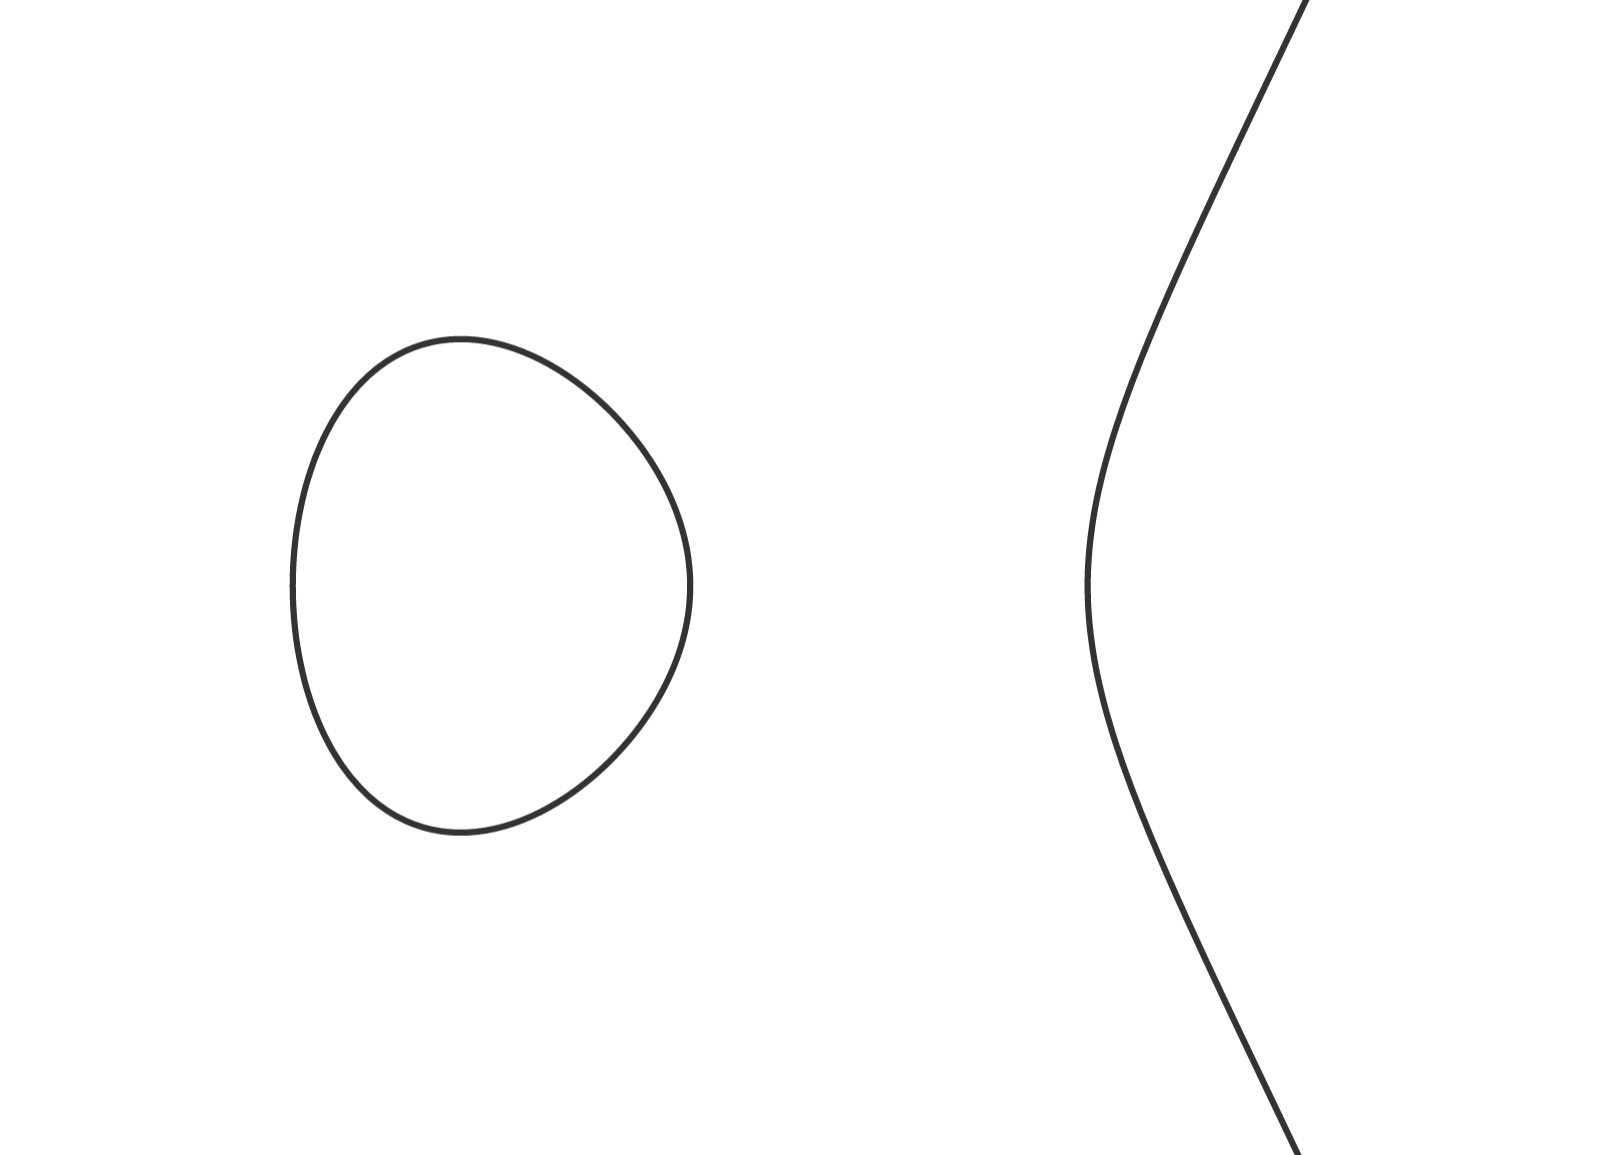
\includegraphics[width=.7\linewidth]{figures/5.png}
        \caption{The elliptic curve $E:y^2=x^3-x$}
        \label{figure-vis1}
        \end{subfigure}%
        \begin{subfigure}{.5\textwidth}
        \centering
        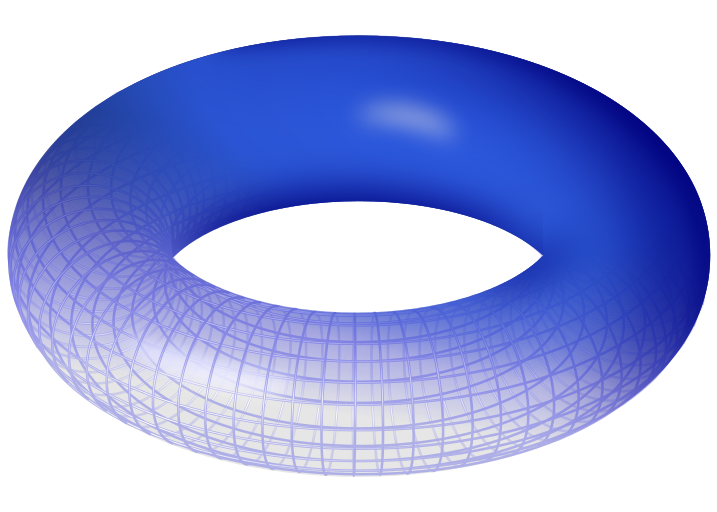
\includegraphics[width=.7\linewidth]{figures/6.png}
        
        \caption{An elliptic curve over $\C$ from \cite{torus}}
        \label{figure-vis2}
        \end{subfigure}
        \end{figure}
        
        In this report, we will first present a series of elementary results on elliptic curves themselves, elliptic curves over $\Q$ and Mordell's theorem concerning the subgroup $E(\Q)$ in some elliptic curve $E$, and some results about elliptic curves over finite fields. Taking a step further, we will define various abstract geometric tools, applying them to elliptic curves over arbitrary fields. This allows us to see why elliptic curves are so useful --- they actually describe a huge family of curves; we could also endow each elliptic curve with an extremely neat abelian structure, algebraically, by creating a map between an elliptic $E$ and the degree-$0$ part of its Picard group $\Pic^0(E)$. Then, the report will present some essential constructions on elliptic curves, including isogenies, Tate modules and Weil parings.
    
        Now let's consider the Riemann $\zeta$ functions, where $\Re s>1$,
        $$\zeta(s)=\sum_{n=1}^\infty \frac{1}{n^s}=\frac{1}{1^s}+\frac{1}{2^s}+\frac{1}{3^s}+\cdots$$
        Euler proved that 
        $$\zeta (s)=\prod_{p\text{ prime}}\frac{1}{1-p^{-s}}$$
        It is possible to define an analytic continuation of $\zeta$ denoted by $\zeta^*$ which satisfies the functional equation
        $$\zeta^\ast(s)=\zeta^\ast(1-s)$$
        The prominent Riemann Hypothesis states that if $\zeta(s)=0$ then $\Re(s)=1/2$ for nontrivial $s$. The Riemann zeta function can be generalized to all number fields, summing over the prime ideals of a number field. The fact that there is very close analogy between curves over a finite field and algebraic number fields motivated Emil Artin to define a zeta function of curves over finite fields. Weil and Hasse used the function $\zeta_C$ as a tool proving the following bound $$|N_m-1-q^m|\leq2gq^{\frac{m}{2}}$$
        where $g$ denotes the genus of the curve $C/\F_q$ and $N_m$ the number of $\F_{q^m}$-rational points on $C$. This is known as the Hasse bound.
        
        Weil subsequently made several conjectures about Artin's zeta function generalized to all projective varieties.
        \[Z(V/\F_q;T)=\exp\left(\sum_{r=1}^\infty \frac{\# V(\F_{q^r})}{r}T^r\right)\]
        He conjectured that the zeta function (1) is a rational function, (2) satisfies a functional equation and (3) a version of Riemann Hypothesis called the $p$-Riemann Hypothesis holds on this zeta function.
        
        The report will follow Hasse's proof of these statements, which is the key motivation that Weil made his conjectures, proving the results for elliptic curves over finite fields. This important result gave rise to many modern theories of geometry and number theory.

        %%%%%% ECC %%%%%%%
        Coming back from pure abstraction to practical applications, we introduce the interaction of elliptic curves and cryptography. Working with elliptic curves on finite fields seems no longer geometric, but it allows us to use elliptic curves as an effective object in cryptography. The cryptosystems in the earlier years often encrypt things using functions on the finite field $\Z/p\Z$, which is rather small. But with the help of elliptic curves, one can use the rational points $E(\F_p)$ instead and can work with a larger domain where we can choose the encryption functions.
 
 
 
 
 

 
 
 
 
 
 
 
 
    %%%%%%%%%%%%%%%%%%%%%%%%%%%%%%%%%%%%%%%%%%%%%
    %%%%%%%%%%%%%%%% Section %%%%%%%%%%%%%%%%%%%%
    %%%%%%%%%%%%%%%%%%%%%%%%%%%%%%%%%%%%%%%%%%%%%
    \newpage
    \section{Basic Algebra}
    %%%%%%%% Subsection %%%%%%%%%%%%
    \subsection{Fields and Galois extensions}\label{ssec-fields}
        \begin{definition}%[Field]
            A \textit{field} $K$ is a commutative ring where every nonzero element is a unit. Suppose $L$ is a larger field containing $K$, then $K$ is said to be a subfield of $L$.
        \end{definition}
        \begin{definition}%[Field Extension]
            If $L$ is a field and $K$ is a subfield of $L$, then $L$ is a \textit{field extension} of $K$, denoted by $L/K$.
        \end{definition}
        By the definition of fields, every extension $L/K$ is a vector space over $K$. One can define the \textit{degree of extension} as
        \[[L:K] := \dim_K(L),\] 
        which is the dimension of this vector space over $K$. For example, $[\C : \R] = 2$, $[\R : \Q] = \infty$. For elements $\alpha_i$ in $L$, we define $K(\alpha_1, ..., \alpha_n)$ to be the minimal subfield of $L$ that contains $K$ and all $\alpha_i$. This is simply the fraction fields of the algebra $K[\alpha_1, ..., \alpha_n]$.
        
        \begin{definition}%[Finite Extension]
            A field extension $L/K$ is said to be \textit{finite} if $[L:K]<\infty$.
        \end{definition}
        
        \begin{definition}%[Algebraic]
            Given field $K$, an element $\alpha$ (not necessarily in $K$) of some field extension $L/K$ is \textit{algebraic} over $K$ if $\alpha$ is root of some polynomial $p(x) \in K[x]$. Otherwise, $\alpha$ is called transcendental. 
        \end{definition}
        \begin{remark}
            Clearly all elements of the ground field $K$ is algebraic over $K$.
        \end{remark}
        \begin{definition}%[Algebraic extension]
            A field extension $L/K$ is called an \textit{algebraic extension} if all elements of $L$ are algebraic over $K$. 
        \end{definition}
        \noindent The following lemma is immediate if we write out the set $\{1,\alpha, \alpha^2,\dots\}$ and argue about its linear dependence.
        \begin{lemma}
            If $M/K$ is a field extension then $\alpha \in M$ algebraic over $K$ if and only if $\alpha$ is contained in a finite extension of $K$.
        \end{lemma}
        \begin{remark}
            This, together with \autoref{corollary-tower-fin-fin}, suggests that $\alpha$ is algebraic if and only if $K(\alpha)/K$ is finite, since it's the smallest field extension of $K$ containing $\alpha$.
        \end{remark}
        \begin{lemma}[Tower theorem]\label{theorem-tower}
            For a tower of fields $M/L/K$, 
            $$[M : K] = [M:L][L:K]$$
            where both sides are either finite or infinite at the same time. 
        \end{lemma}
        \begin{proof}
            The case where one extension is infinite is clear, as we have an infinite set of elements linearly independent over $K$. 
            
            Now suppose both $L/K$ and $M/L$ are finite. Choosing a basis for $L$ over $K$, say $\{a_1, ...,  a_r\}$ and a basis of $M$ over $L$, say $\{b_1, ..., b_s\}$. Then the set of  products $b_i a_j$ can be shown to be linearly independent in $M$ and spans $M$. So the dimension of $M$ over $K$ is just $rs = [M:L][L:K]$. 
        \end{proof}
        
        \begin{corollary}\label{corollary-tower-fin-fin}
            For a tower of fields $M/L/K$, $L/K$ and $M/L$ are finite if and only if $M/K$ is finite.
        \end{corollary}
        
        \begin{corollary}
            Given a field extension $L/K$, if $\alpha, \beta \in L$ are algebraic over $K$, then $\alpha + \beta, \alpha \beta, \alpha - \beta, \alpha/\beta$ (if $\beta \neq 0$) are all algebraic over $K$. 
        \end{corollary}
        \begin{proof}
            Note $K(\alpha, \beta)/K(\alpha)/K$ where each extension is finite as      $\alpha, \beta$ are algebraic. Thus, $K(\alpha, \beta)/K$ is finite which contains $\alpha + \beta, \alpha \beta, \alpha - \beta, \alpha/\beta$.
        \end{proof}
        
        For an arbitrary polynomial $p(x)$ over field $K$, one may wonder if there is always a field $L$ where $f$ has a root in $L$, and if there is a field $M$ in which $f$ splits into linear factors. And one can ask if a smallest such field exists.
        \begin{definition}%[Splitting Field]
            A field $M/K$ is the \textit{splitting field of a polynomial $p(x)\in K[x]$} if $M$ is the smallest among fields where $p(x)$ splits into linear factors in $M$.
        \end{definition}
        \begin{remark}
            If $\alpha_1,\dots,\alpha_n$ are roots of $p$ in $M$, then $M=K(\alpha_1,\dots,\alpha_n)$.
        \end{remark}
        
        \begin{lemma}%[Existence of splitting field]
            Given a field $K$ and $f\in K[x]$, there is some finite $L/K$, unique up to isomorphism, where $f$ splits.
        \end{lemma}
        \noindent The isomorphisms between splitting fields may not be unique. Splitting fields can be defined on any set of polynomials. When we define it on the whole polynomial ring $K[X]$, we get an algebraic closure.
        \begin{definition}
            An field $L$ is \textit{algebraically closed} if all polynomials in $L[x]$ have roots in $L$. 
        \end{definition}
        \begin{definition}%[Algebraic closure]
            Given a field $K$, an algebraic extension $L/K$ is called an \textit{algebraic closure} of $K$ if it is algebraically closed.
        \end{definition}
        \noindent Algebraic closures are unique up to isomorphisms. Therefore, in the following section we denote the ground field by $k$ and its algebraic closure by $K$.
        
        Using Zorn's lemma we obtain
        \begin{theorem}
            Any field $k$ has an algebraic closure.  
        \end{theorem}
        In an algebraic extension, we have the following theorem:
        \begin{theorem}
            The following statements are equivalent for an algebraic extension $L/k$
            \begin{enumerate}[\normalfont(i)]
                \item Any polynomial $p \in k[x]$ that is irreducible and has a factor in $L$ factors into linear factors in $L[x]$. i.e. if any one root is in $L$, then all other roots are in $L$.
                \item $L$ is the splitting field of some set of polynomials over $k$. 
                \item Extend $L$ to algebraic closure $K/k$ containing $L$. Any automorphism of $K$ that fixes all elements of $k$ maps $L$ to $L$.
            \end{enumerate}
            If an algebraic extension $L/k$ satisfies any of the statements above, it is said to be \textup{a normal extension of $k$}
        \end{theorem}
        
        \begin{lemma}
            Any algebraic extension $L/k$ of index $2$ is normal.
        \end{lemma}
        \begin{proof}
            Since $[L:k]=2$, $L = k(\alpha)$ for some $\alpha$, and $\alpha^2 + b \alpha + c = 0$ for some $b, c \in k$. If $\beta$ is another root of this polynomial, we have $\beta + \alpha = -b$, meaning $\beta = -b - \alpha \in L$. So the extension is normal.  
        \end{proof}
        \begin{example}
            One may wish that if $M/L, L/k$ are normal, then $M/k$ is normal. But consider $k = \Q$, $L = \Q(\sqrt{2})$, $M = \Q(\sqrt[4]{2})$, each extension $L/k$, $M/L$ has degree $2$ so they must be normal. But the polynomial $x^4 - 2 \in k[x]$ has roots $\pm \sqrt[4]{2}$ and $\pm \sqrt[4]{2} i$. The last two roots are complex, so they cannot be in       $M$, meaning $M/k$ is not normal. 
        \end{example}
        
        \begin{definition}%[Separable polynomial]
            A polynomial $p(x) \in k[x]$ is \textit{separable} if it factors over the algebraic closure $K$ as $\prod (x-\alpha_i)$ where $\alpha_i$ are all distinct. i.e. there is no repeated root. This is equivalent to $\gcd(p, p') = 1$ in $k[x]$.
        \end{definition}
        
        \begin{definition}%[Separable Extension]
            Given field extension $L/k$, an element $\alpha \in L$ is \textit{separable} over $k$ if it is root of a separable polynomial in $k[x]$. If all elements of $L$ is separable, $L/k$ is a \textit{separable extension}. 
        \end{definition}
        \noindent So for $L/k$, given an irreducible polynomial $f \in k[x]$ of degree $n$ with $\alpha \in L$ being one of its roots, if $k \subseteq L$ is normal, then $f$ has $n$ roots in $L$; if further $L/k$ is separable, $f$ has $n$ distinct roots in $L$.
        \begin{lemma}%[Finite field extension]
            All finite field extensions $\F_{p^m}/\F_{p^n}$ (where $m\geqslant n$) are separable
        \end{lemma}
        \begin{proof}
            Recall all elements of $\F_{p^m}$ are roots of $f=x^{p^m} - x$. Since $p^n\mid p^n$, $f' = -1$ and $\gcd(f, f') = 1$, meaning $f$ is separable. So this extension is separable.
        \end{proof}
        
        \begin{definition}%[purely inseparable]
            A field extension $L/k$ is \textit{purely inseparable} if any $\alpha \in L$ is a root of $x^{p^n} - a$ for some $a \in k$. Over $K$, this polynomial equals $\left(x-\sqrt[p^n]{a}\right)^{p^n}$, which is far from having distinct roots. 
        \end{definition}
        
        \begin{theorem}\label{theorem-sep-exist}
            For any field extension $L/k$, there is a field $k^{\text{sep}}$ s.t. $k^{\text{sep}}/k$ is separable extension and $L/k^{\text{sep}}$ is purely inseparable extension. 
        \end{theorem}
        \noindent In fact, $k^{\text{sep}}$ is just the field consisting of all separable elements of $L$. Now we define \textit{Galois extensions} in several equivalent ways
        \begin{theorem}
            The following are equivalent for the extension (not necessarily finite) $M/k$ and \textup{the Galois group} $G=\Gal(M/k) = \{\s\in\Aut(M):\forall x\in k, \s(x)=x\}$
            \begin{enumerate}[\normalfont(i)]
                \item The extension is algebraic, normal and separable.
                \item The \textup{fixed field} $M^G =\{x\in M:\forall \s\in G, \s(x)=x\}$ (which is a subfield of $M$) is $k$.
                \comment{
                %%%%%%%% Probably don't need these statements. Will see later. %%%%%%%%%%%%%%
                \item $M$ is splitting field of a separable polynomial. 
                \item For the collection of fields $L$ s.t. $k \subseteq L \subseteq M$ and collection      of groups $H$ s.t. $1 \subseteq H \subseteq G$, there is a one-to-one         correspondence(called \textit{Galois correspondence}) between these two collections.        Namely $L \mapsto \text{Gal}(M/L)$ and $H \mapsto M^H$, these are inverses to each        other, and they are order reversing (e.g. larger field $L$ results in smaller $M/L$, so        $\text{Gal}(M/L)$ is smaller. ) }
            \end{enumerate}
        \end{theorem}
        The Galois group of some fields are easier: 
        \begin{definition}%[Perfect field]
            A field $k$ is \textit{perfect} if one of following equivalent conditions holds: 
            \begin{enumerate}[\normalfont(i)]
                \item Every irreducible polynomial over $k$ is separable.
                \item Every algebraic extension of $k$ is separable.
            \end{enumerate}
        \end{definition}
    \noindent Therefore, if $k$ is a perfect field, the Galois group $\Gal(K/k)$ only fixes $k$ where $K$ is an algebraic closure of $k$ (thus algebraic and normal; and $K$ is separable as $k$ is perfect).
    
    %%%%%%%% Subsection %%%%%%%%%%%%
    \subsection{Miscellaneous}
    \begin{lemma}\label{lemma-cauchy-schwartz}
        Suppose $A$ is an abelian group and $d:A\to\Z$ a positive definite quadratic form. Then
        \[|d(a-b)-d(a)-d(b)|\leqslant2\sqrt{d(a)d(b)}\]
        for all $a, b\in A$.
    \end{lemma}
    \begin{proof}
        If $a=0$ then we are done. Suppose $a\neq 0$. Let $L(a, b)=d(a, b)-d(a)-d(b)$ which is a $\Z$-bilinear form. Then since $d$ is positive definite, for all $m,n\in\Z$,
        \[0\leqslant d(ma-nb)=m^2d(a)+mnL(a,b)+n^2d(b)\]
        Let $m=-L(a,b)$ and $n=2d(a)$. We obtain
        \[d(a)\left(4d(a)d(b)-L(a, b)\right)\geqslant 0\]
        which gives the result as $a\neq 0$.
    \end{proof}
    
    %%%%%%%%%%%%%%%%%%%%%%%%%%%%%%%%%%%%%%%%%%%%%
    %%%%%%%%%%%%%%%% Section %%%%%%%%%%%%%%%%%%%%
    %%%%%%%%%%%%%%%%%%%%%%%%%%%%%%%%%%%%%%%%%%%%%
    \section{Basic Algebraic Geometry}
    %%%%%%%% Subsection %%%%%%%%%%%%
    \subsection{Affine varieties}
        Given an algebraically closed field $K$, we define the affine $n$-space to be 
        $$\Ac^n(K) = \{(x_1, \cdots, x_n) \, : \, x_i \in K\}$$
        namely the set of $n$-tuples of elements of $K$. When the field used is clear, $\Ac^n$ is used instead. For any polynomial $f \in K[X_1, \cdots, X_n]$, it naturally defines a map $f : \Ac^n \rightarrow K$ by $(x_1, \cdots, x_n) \mapsto f(x_1, \cdots x_n)$. This $f$ is usually called a \textit{polynomial function}.

        \begin{definition}%[Hypersurface]
            Given set of polynomials $S \subset K[X_1, \cdots , X_n]$, an \textit{an affine algebraic set} is a set of the form
            $$\mathbb V(S) = \{x \in \Ac^n : f(x) = 0, \forall f \in S\}$$
            if $S = \{f_1,\dots,f_n\}$, we write $\mathbb V(f_1,\dots,f_n)$ instead. We call a set $X\subseteq\A^n$ \textit{algebraic} if $X =\mathbb V(S)$ for some set $S$.
        \end{definition}
        \noindent Some basic algebraic geometry results:
        \begin{theorem}%[Key properties of hypersurfaces]
            \begin{enumerate}[\normalfont(i)]
                \item $\mathbb V(0) = \Ac^n$. If $K$ is infinite, $\mathbb V(K[X_1, \cdots, X_n]) = \emptyset$.
                \item If $I = (S)$ (the ideal generated by $S$), $\mathbb V(S) = \mathbb V(I)$
                \item If $\{I_\alpha\}$ is a collection of ideals, $\mathbb V(\bigcup_\alpha I_\alpha)=         \bigcap_\alpha \mathbb V(I_\alpha)$. 
                \item If $I \subseteq J$, then $\mathbb V(I) \supseteq \mathbb V(J)$
                \item For ideals $I_1, I_2$, $\mathbb V(I_1 \cap        I_2) = \mathbb V(I_1) \cup \mathbb V(I_2)$. 
            \end{enumerate}
        \end{theorem}
        
        \begin{definition}%[Ideal of $X$]
            Given subset $X \subseteq \Ac^n$, the \textit{ideal of $X$} is 
            $$\mathbb I(X) = \{F \in K[X_1, \cdots X_n] : F(a_1, \cdots, a_n)=0, \forall (a_1, \cdots,         a_n) \in X\}$$
        \end{definition}
        
        \begin{definition}%[Irreducible Algebraic set]
            If $V = V_1 \cup V_2$, for some proper subsets $V_1, V_2$ of $V$, then $V$ is called \textit{reducible}. Otherwise $V$ is called \textit{irreducible}. An irreducible algebraic set is an \textit{affine variety}. 
        \end{definition}
        
        \begin{lemma}
            $V$ is irreducible if and only if $\mathbb I(V)$ is prime. 
        \end{lemma}
        \comment{
        \begin{proof}
            We use contra-positive statement. \\
            Assume $I(V)$ is not prime, there are polynomials $F_1, F_2$ s.t. $F_1 F_2 \in I(V)$, but         $F_i \not\in I(V)$. For any $x \in V$, $F_1F_2(x) = F_1(x)F_2(x) = 0$ so $x \in V(F_1)$ or      $V(F_2)$. So $V \subseteq V(F_1) \cup V(F_2)$ and we can split $V$ into two parts: $V = (V      \cap V(F_1)) \cup (V \cap V(F_2))$. By condition $F_i \not\in I(V)$, $V \cap V(F_i) \neq V$.      So $V$ is reducible. \\
            Now assume $V$ is reducible, $V = V_1 \cup V_2$. Then $I(V_i) \supset I(V)$. Pick $F_i \in         I(V_i)$ s.t. $F_i \not\in I(V)$, then $F_1 F_2 \in I(V)$. So $I(V)$ is not prime. 
        \end{proof}}
        \comment{
        \begin{thm}[Decomposition]
            For any algebraic $V \subset \Ac^n$, there are unique irreducible algebraic sets $V_1,      \cdots V_m$ s.t. $V = V_1 \cup \cdots \cup V_m$ and $V_i \not\subset V_j$ for $i \neq j$.
        \end{thm}
        $V_i$ are called \textit{irreducible components} of $V$. 
        
        \begin{prop}
            If $V \subset \Ac^n$ is algebraic, then following are equivalent
            \begin{enumerate}
                \item $V$ is irreducible
                \item For any non-empty open sets $U_1, U_2 \subset V$, $U_1 \cap U_2 \neq \emptyset$. 
                \item Any non-empty open set $U \subset V$ is dense.
                %%%%%%%% Cannot have dense sets without a topology
            \end{enumerate}
        \end{prop}
        \begin{proof}
            For $U_1, U_2 \neq \emptyset$, $U_1 \cap U_2 = \emptyset \Leftrightarrow V = (V \setminus       U_1) \cup (V \setminus U_2)$ $\Leftrightarrow$ we have a non-trivial decomposition of $V$        $\Leftrightarrow$ $V$ is reducible. 
            Equivalence of 2, 3 follows from $U$ is dense in $V$ iff $U$ meets every open set in $V$.
        \end{proof}}
        

        
        \comment{
        \subsubsection{Polynomial map}
        
        Given algebraic set $V \subset A^n(K)$, with $I(V)$ being ideal of $V$. We wish to define polynomial functions $f : V \rightarrow k$. We have mentioned that every polynomial in $K[X_1, \cdots, X_n]$ corresponds to a polynomial function. And if $F, G \in K[X_1, \cdots, X_n]$       corresponds to the same polynomial function, $F(P) = G(P) \forall P \in V$, that means $F - G       \in I(V)$. Therefore,
        $$K[V] := \{\text{polynomial functions}\} \equiv \frac{K[X_1, \cdots, X_n]}{I(V)}$$
        $K[V]$ is the \textit{coordinate ring}. There is a correspondence between $\{\text{ideals }I  \subset K[V]\}$ and $\{X \subset V\}$ given by $I \mapsto V(I)$ and $X \mapsto I(X)$.}
        
        \begin{definition}%[coordinate ring]
        The \textit{coordinate ring} of a subset $V$ of $\mathbb P^n$ is the quotient
        \[K[V]=K[x_1,\dots,x_n]/\mathbb I(V)\]
        which is an integral domain if $V$ is an (affine) variety.
        \end{definition}
        
        Define the \textit{Zariski Topology} on $\Ac^n$ by taking the algebraic sets as closed sets. It is indeed a topology by the key properties of algebraic sets. The Zariski topology on $\Ac^n$ induces a topology on any subset $W \subset \Ac^n$ by defining it to be the subspace topology on $W$. If $V$ is irreducible (i.e. $V$ is variety), $W$ is a \textit{subvariety} of $V$ if it is an irreducible closed subset of $V$. %%% You can only talk about closed subsets if you have the subspace topology. Therefore the term "closed subsets" would suffice
        
        %%%%%%%%%%%%%%%% TO discuss: appendix or not?
        \comment{
        \begin{definition}
            Given algebraic sets $V, W$, a regular map $f: V\to W$ is a map with $F_1, \cdots, F_m \in K[X_1, \cdots, X_n]$ s.t. 
            $$f(P) = (F_1(P), \cdots, F_m(P))$$
        \end{definition}
        
        By defining $f_j := \pi_j \circ f$ (where $\pi_j(X) = $ jth coordinate of $X$), we can write $f = (f_1, \cdots, f_m)$ and $f$ is polynomial map iff $f_i$ are polynomial functions. 
        \begin{definition}[Isomorphism]
            $f : V \rightarrow W$ is isomorphism between two algebraic sets if there is a polynomial map $g$ s.t. $f \circ g = g \circ f = id$. 
        \end{definition}
        
        \comment{
        Motivated by cross product in $\R^3$, a concept stronger than vector space is defined. 
        
        \begin{definition}[Algebra]
            A ring $A$ is $R$-algebra($R$ is ring) if it is $R$ module s.t. ring multiplication $\cdot$ on $A$ becomes a bilinear operator between elements of $R$. i.e. for all $x, y, z \in R$ and $a, b \in K$: 
            \begin{itemize}
                \item $(x+y) \cdot z = x \cdot z + y \cdot z$
                \item $x \cdot (y + z) = x \cdot y + x \cdot z$ 
                \item $(ax) \cdot (by) = (ab) (x \cdot y)$
            \end{itemize}
            The first two conditions for bilinear operator are automatically satisfied by a ring        (distributivity), so only thing to check is the third one. 
        \end{definition}
        
        Note coordinate ring $k[V]$ is a $k$-algebra. \\
        \\
        We have the following result relating algebra to coordinate rings
        
        \begin{prop}
            $K$-algebra $A$ is isomorphic to $k[X]$ for some algebraic set $X$ $\Leftrightarrow$ $A$ is      affine ($A$ is finitely generated), reduced(no nilpotent elements). 
        \end{prop}
        
        \begin{definition}[Algebra homomorphism]
            $R$-algebra homomorphism $\phi : A \rightarrow B$ is a $R$-module homomorphism that         satisfies 
            $$f(a \cdot b) = f(a) \cdot f(b)$$
        \end{definition}}
        
        The polynomial maps defines isomorphism between algebraic sets and surprisingly they corresponds         to k-algebra homomorphisms between coordinate rings 
        
        \begin{thm}
            Polynomial map $f : V \rightarrow W$ naturally induce a k-algebra homomorphism $f^* : k[W]        \rightarrow k[V]$. And one can also find a polynomial map for each k-algebra homomorphism        from $k[W]$ to $k[V]$. i.e. $f \rightarrow f^*$ is a bijection. \\
            And if $f : V \rightarrow W, \, g : W \rightarrow U$ are polynomial maps, $(g \circ f)^* =       f^* \circ g^*$. 
        \end{thm}
        \begin{proof}
            \textcolor{red}{Under Construction}
        \end{proof}
        
        
        \subsubsection{Zariski Topology}
        \begin{definition}[Zariski Topology]
            \textit{Zariski Topology} on $\Ac^n(K)$ is defined by $U$ is open if $\Ac^n \setminus U$ is algebraic set. (So algebraic sets of $\Ac^n$ are closed)
        \end{definition}
        It is indeed a topology by key properties of hypersurface. Zariski topology on $\Ac^n$ induces a Zariski topology on any algebraic set $X \subset \Ac^n$, by defining it to be the subspace topology on $X$ with closed sets being algebraic subsets of $X$. 
        
        \begin{definition}[Irreducible, connected]
            If $X = X_1 \cup X_2$  where $X_i \neq X$ and $X_i$ are closed, disjoint. (equivalently,         $X_i$ are open, disjoint). Then $X$ is \textit{disconnected}. Otherwise, $X$ is         \textit{connected}. \\
            If $X = X_1 \cup X_2$  where $X_i \neq X$ and $X_i$ are closed, then $X$ is         \textit{reducible}. Otherwise, $X$ is \textit{irreducible}
        \end{definition}
        Every irreducible space is connected, but not conversely. \\
        Zariski topologies are usually more coarse (have less open sets) than metric induced topologies.         $\Ac^1(K)$ is irreducible for any infinite field $K$, because the only algebraic sets of $V$ are       the finite sets. So if $\Ac^1(K) = X_1 \cup X_2$ where $X_i$ are closed, $\Ac^1(K)$ is finite.       And it is not Hausdorff as the open neighbourhood in this case are co-finite sets or         $\emptyset$. 
        
        \begin{prop}
            In any irreducible topological space $X$, any non-empty open set is dense in $X$
        \end{prop}
        \begin{proof}
            If $U \subset \overline{U} \subset X$. Then $X = \overline{U} \cup (X \setminus U)$, which is a union of two closed sets not equal to $X$. This contradicts irreducibility. 
        \end{proof}
            
        %%%%%%%% Subsection %%%%%%%%%%%%
        \subsection{Projective plane}
        Algebraically, the projective plane $\Pc^2$ can be introduced by solutions of Fermat equations:
        $$x^N + y^N = 1\text{(first)}, \quad X^N + Y^N = Z^N \text{(second)}$$
        Using basic number theory, it turns out that if $x = \frac{a}{c}, \; y = \frac{b}{d}$ (in lowest      term) with $c, d > 0$ and $a, b, c, d \in \Z$ is a pair of rational solutions to Fermat's first      equation, then $c = d$. \\
        So all solutions are of the form $(\frac{a}{c}, \frac{b}{c})$, which gives a solution $(a, b,      c)$ to Fermat's second equation. Conversely, if $(a, b, c)$ is a solution to second equation,       $(\frac{a}{c}, \frac{b}{c})$ is a solution to first equation. But also, for any $0 \neq t \in       \Z$, $(ta, tb, tc)$ corresponds to the same solution of Fermat's first equation. So we define      equivalence relation 
        $$(a, b, c) \sim (a', b', c') \text{ iff there is non-zero integer } t \text{ s.t. } a' = ta, b'      = tb, c' = tc$$ 
        But we discard solution $(0, 0, 0)$ to second equation. Note for $N$, the solution $(\pm 1, \mp         1, 0)$ to second Fermat equation corresponds to special solution $(\infty, \infty)$ to first        equation. So now we can define the projective plane: 
        $$\Pc^2 := \frac{[a, b, c] \, : \, a, b, c \text{ not all zero}}{\sim}$$
        set of equivalence classes $[a, b, c]$ where $a, b, c$ are not all zero, and $a, b, c$ are      called homogeneous coordinates. A general version is given below: 
        
        \begin{definition}[projective n-space]
            $$\Pc^n := \frac{[a_0, a_1, ..., a_n] \, : \, a_0, ..., a_n \text{ not all zero}]}{\sim}$$
        \end{definition}
        
        \begin{definition}[line on $\Pc^2$]
            A line is the set of points $[a, b, c] \in \Pc^2$ satisfying equation of the form 
            $$\alpha X + \beta Y + \gamma Z = 0$$
            where $\alpha, \beta, \gamma$ are not all zero. 
        \end{definition}
        
        If a point is on a line, all homogeneous coordinates are on that line. \\
        \\
        Projective plane can also be introduced geometrically. In order for the law "two distinct lines       have exactly one intersection" to hold even for parallel lines, points at infinity are defined.        But we need one point at infinity for all directions, as two distinct parallel lines can only         have one intersection at infinity. So projective plane is defined as 
        $$\Pc^2 = \Ac^2 \cup \{\text{set of directions}\}$$
        where $\Ac^2 = \Ac^2(\R)$ is the affine space, and each direction corresponds to a point at         infinity. Set of all points at infinity form a line $L_\infty$. This projective space has nice        properties:
        \begin{itemize}
            \item There is a unique line going through two distinct points in $\Pc^2$. (Including points      at infinity)
            \item Two distinct lines intersect at exactly one point. 
        \end{itemize}
        
        Every line is parallel to a unique line through origin, say $Ay = Bx$, so we can define set of      points $[A, B]$ to be set of directions with equivalence relation $(A, B) \sim (A', B')$ if $A'         = tA, B' = tB$ for some non-zero $t$. One can immediately recognise that set of directions have      the same structure as $\Pc^1$(algebraic definition). So in fact $\Pc^2 = \Ac^2 \cup \Pc^1$. 
        
        \begin{prop}[Equivalence]
            Algebraic definition and geometric definitions of $\Pc^2$ are equivalent. 
        \end{prop}
        \begin{proof}
            We can assign $[a, b, c]$ (in algebraic definition) to $(a/c, b/c) \in \Ac^2$ if $c \neq 0$,         and if $c = 0$(represents point at infinity), send it to $[a, b]$ instead. This is a map        from algebraic definition of $\Pc^2$ to $\Ac^2 \cup \Pc^1$. \\
            \\
            For the other direction, send $(x, y) \in \Ac^2$ to $[x, y, 1]$ and $[A, B] \in \Pc^1$ to      $[A, B, 0]$. Then this is a map from $\Ac^2 \cup \Pc^1$ to algebraic definition of $\Pc^2$.         \\
            Indeed the above two maps are inverse to each other(can be checked case by case), so        equivalence of two definitions is proved. 
        \end{proof}
        
        Main Source for this subsection: Silverman and Tate, Appendix A}
        
        
    %%%%%%%%%%%%%%%% subsection %%%%%%%%%%%%%%%%%%%%
    \subsection{Projective varieties}
        In order for any two lines in affine space to have intersection, even parallel ones, we need the following definition
        %%% The notation P^n(k) is reserved for the k-rational points in P^n. Use big K in this section.
        \begin{definition}
            The \textit{projective $n$-space over $K$} $\Pc^n = \Pc^n(K)$ is the set of all lines through origin in $\Ac^{n+1}$. Equivalently, $\Pc^n$ is set of equivalence classes on $\Ac^{n+1} \setminus \{0\}$ under equivalence relation 
            $$(x_0, \cdots, x_{n}) \sim (y_0, \cdots, y_{n}) \mbox{ if and only if }\exists \lambda\in K^*, y_i = \lambda x_i,\forall i$$
            The equivalence class of $(x_0, \cdots, x_{n})$ is denoted by $[x_0: \cdots: x_{n}]$.
        \end{definition}
        \noindent Given a homogeneous polynomial $F \in K[x_0, \cdots, x_{n}], P \in \Pc^n$, $F(P) = 0$ means $F(x_0, \cdots, x_{n}) = 0$ for any choice of Representatives of $P$. With this definition, we can move the definition of algebraic sets to the projective space (called \textit{an projective algebraic set in $\Pc^n$}) $\mathbb V(S) = \{P \in \Pc^n :F(P)=0,\forall F \in S\}$ where $S$ is a set of homogeneous polynomial in $K[x_0,\dots, x_n]$. An irreducible projective algebraic set is called a \textit{projective variety} (subvariety defined in the same way). The Zariski topology can also be defined on $\Pc^n$ by taking projective algebraic sets as closed sets.

    
    %%%%%%%%%%%%%%%%%%%%%%%%%%%%%%%%%%%%%%%%%%%%%
    %%%%%%%%%%%%%%%% Section %%%%%%%%%%%%%%%%%%%%
    %%%%%%%%%%%%%%%%%%%%%%%%%%%%%%%%%%%%%%%%%%%%%
    \section{Elliptic Curves}
        One might be surprised that the origin of elliptic curves, one of the most essential objects of modern number theory, came out of the study of calculus --- the study of elliptic integrals, where they got their names \cite{stevenhagen_1997_kernvak}. After years of study, people realized that smooth curves of genus one with a rational point can be classified easily with a simple form of equations.
    %%%%%%%% Subsection %%%%%%%%%%%%
    \subsection{Weierstrass normal forms}
        Recall that we have a perfect field $k$ and its algebraic closure $K$, and we will continue to use these notations in the rest of the report. In this section we assume that $\operatorname{char} k\neq 2, 3$, A cubic is the zero locus of some homogeneous polynomial $f(x,y,z)$ of degree 3 in $\Pc^2$. Any cubic $C$ (possibly singular) can be transformed into a specific form known as the \textit{Weierstrass normal form}. Note the proof here is a bit sketchy, since there is a detailed construction of the Weierstrass equation for curves of genus one in \autoref{theorem-ecg1}.
        
        We choose a coordinate for the projective plane as follow: 
        \begin{enumerate}[\normalfont(1)]
            \item Fix a $k$-rational point $\mathcal{O}$ on a cubic $C$. Define $Z = 0$ to be the tangent line of $C$ at $\mathcal{O}$. 
            \item Define $X = 0$ to be the tangent line of $C$ at the third intersection of $Z=0$ and the cubic. 
            \item Define $Y = 0$ to be any line going through $\mathcal{O}$ other than $Z = 0$. 
        \end{enumerate}
        Dehomogenizing, we get the equation 
        $$y^2+a_1xy+a_3y=x^3+a_2x+a_4x+a_6$$
        Some linear transformations (with the assumption that $\operatorname{char} k\neq 2, 3$) yield the \textit{Weierstrass normal form of $C$}
        $$y^2 = x^3 + ax^2 + bx + c.$$ 
        If the roots of the RHS are distinct, the cubic curve $C$ is called an \textit{elliptic curve}.      Homogenizing this form, we have
        $$Y^2Z = X^3 + aX^2Z + bXZ^2 + cZ^3$$ 
        which intersection with the line $Z=0$ is $X^3 = 0$, with a triple root at $[0:1:0]$. So we have a unique point at infinity, which is non-singular. The group law of cubics in Weierstrass normal forms is usually built on this fixed base point. Due to the presence of $y^2$ on one side, any vertical line only meets the cubic in affine plane at two points, so the third point of intersection must be $\mathcal{O}$.
        
        We are mostly interested in the cases where $a,b,c\in k$ in the Weierstrass normal form of a elliptic curve $E$ (which is equivalent to saying that $E/k$ defined earlier).
        \comment{
        Therefore, $P + Q$ becomes the      reflection point of $P * Q$ about $x$-axis. And $-Q$ is simply reflection point of $Q$ about        $x$-axis.\\
        Simple algebra yields the explicit formulae for $P * Q$: if $P = (x_1, y_1), \; Q = (x_2, y_2)$       and $P * Q = (x_3, y_3)$, then 
        $$x_3 = \lambda^2 - a - x_1 - x_2, \; y_3 = \lambda x_3 + \nu$$
        where $\lambda = \frac{y_2 - y_1}{x_2 - x_1}, \nu = y_1 - \lambda x_1 = y_2 - \lambda x_2$ make        sure that $y = \lambda x + \nu$ is equation of the line joining $P, Q$. This explicit formulae       generalises to finite field $\F_p$ where geometric definition of group law is not possible. If         $P = Q$, $\lambda$ is the tangent at $P$ instead, which is
        $$\lambda = \left.\frac{dy}{dx}\right|_{P_0} = \frac{f'(x_0)}{2y_0}$$  
        to get $P + Q$, simply take $(x_3, -y_3)$. }
        
    
    %%%%%%%%%%%%%%%% subsection %%%%%%%%%%%%%%%%%%%%
     \subsection{The geometric group law}
        In mid-1900s, Weierstrass already made several geometric observations linking the addition of elliptic functions to the addition of points on elliptic curves \cite{conifold_2016_who}. In 1896, Juel presented the formulas for adding points on elliptic curves, and explicitly described elliptic curves as groups \cite{Juel1896}.
        
        There are two possible (and equivalent) definitions/constructions that endow an elliptic curve with an abelian structure, and we aim to include both in this report. As before, an easier and geometric but hard to prove definition is first presented. The \textbf{algebraic construction} and the equivalence of the two constructions are addressed and proved in \autoref{ssec-alg-group}

        By Bézout theorem, the intersection of any line and any elliptic curve consists of three points, counting multiplicities.
        
        Given an elliptic curve $E$ with base point $[0:1:0]$ and two distinct points $P, Q$ on it, we can define a composition $P*Q$ to be the third point of intersection of the line joining $P, Q$ with the cubic. Note that if $P, Q$ are $k$-rational points, the line passing them is defined over $k$. If $E/k$, then the point $P* Q$ is also $k$-rational as it's described by two equations with rational coefficients. If $P = Q$, then let $P* P$ be the other intersection of the tangent line $L$ at $P$ and $E$. Unfortunately, there is no identity element for this composition law. Therefore, we fix a rational point $\mathcal{O}$ on $E$, and define $P \oplus Q$ to be the third intersection of the line joining $P * Q$ and $\mathcal{O}$. Now we have $P \oplus \mathcal{O} = \mathcal{O} \oplus P = P$.
        \begin{figure}[h]
        \centering
        \begin{subfigure}{.5\textwidth}
        \centering
        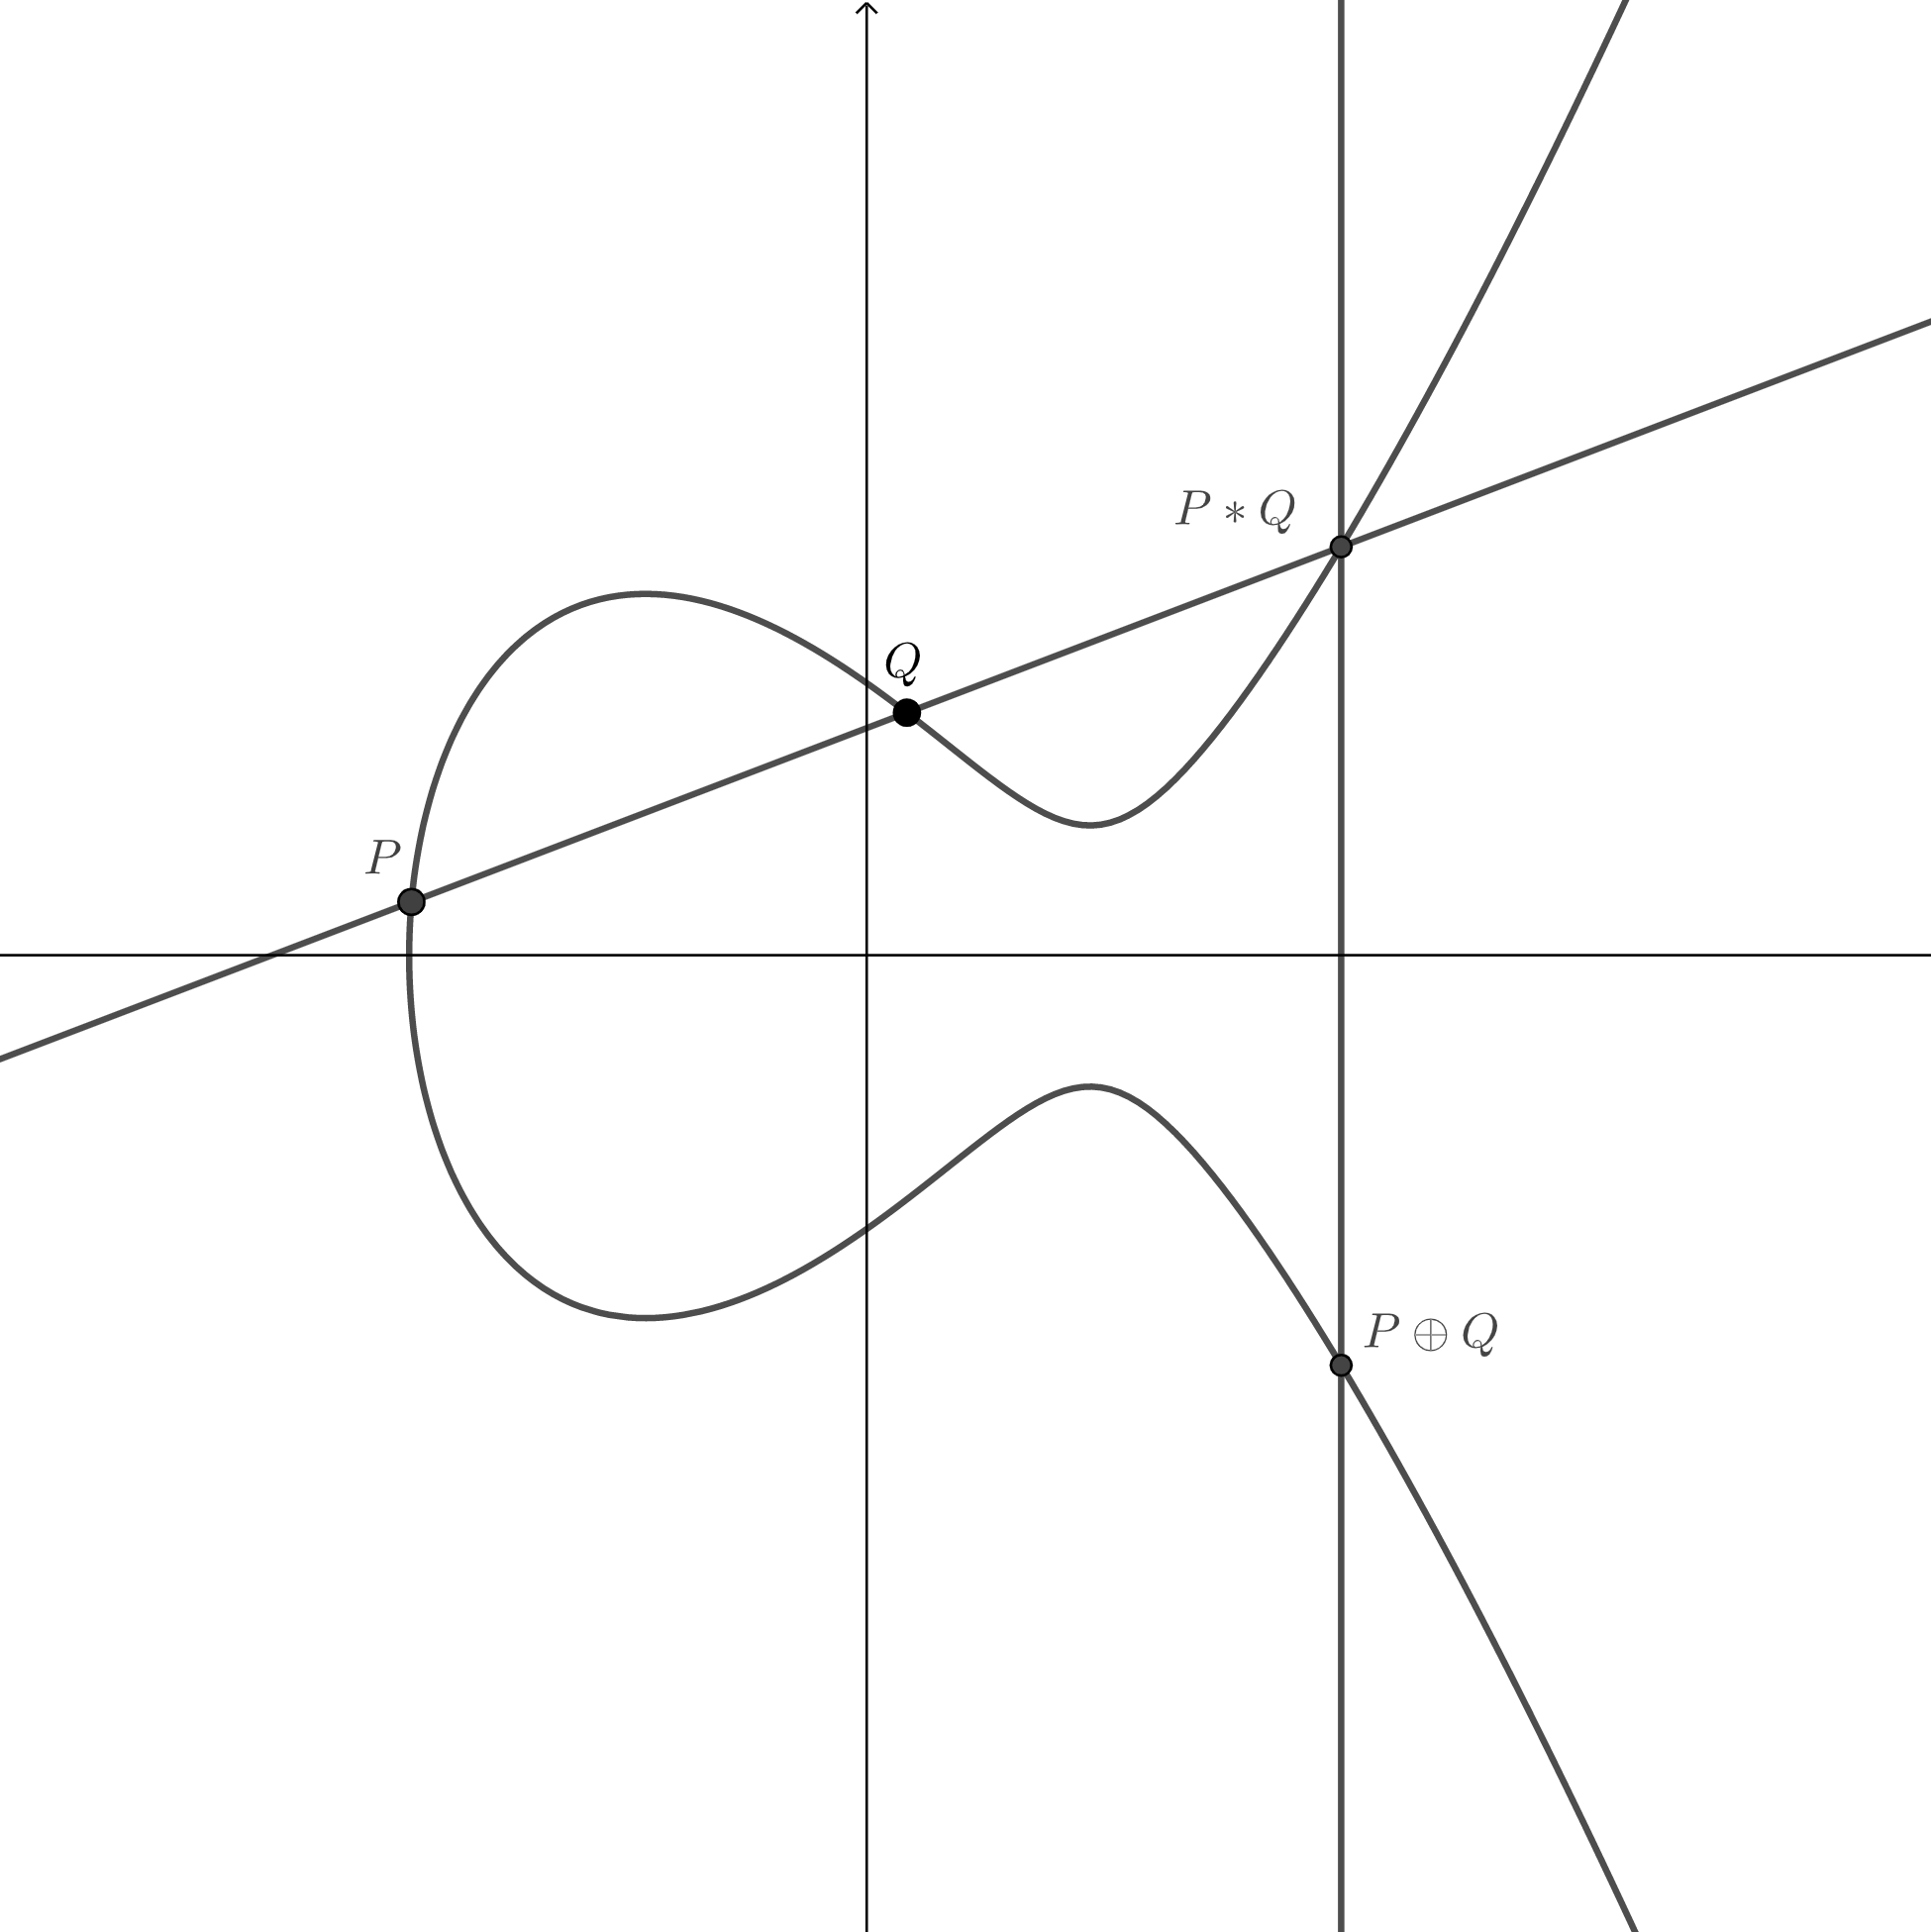
\includegraphics[width=.7\linewidth]{figures/1.png}
        \caption{$P\oplus Q$}
        \end{subfigure}%
        \begin{subfigure}{.5\textwidth}
        \centering
        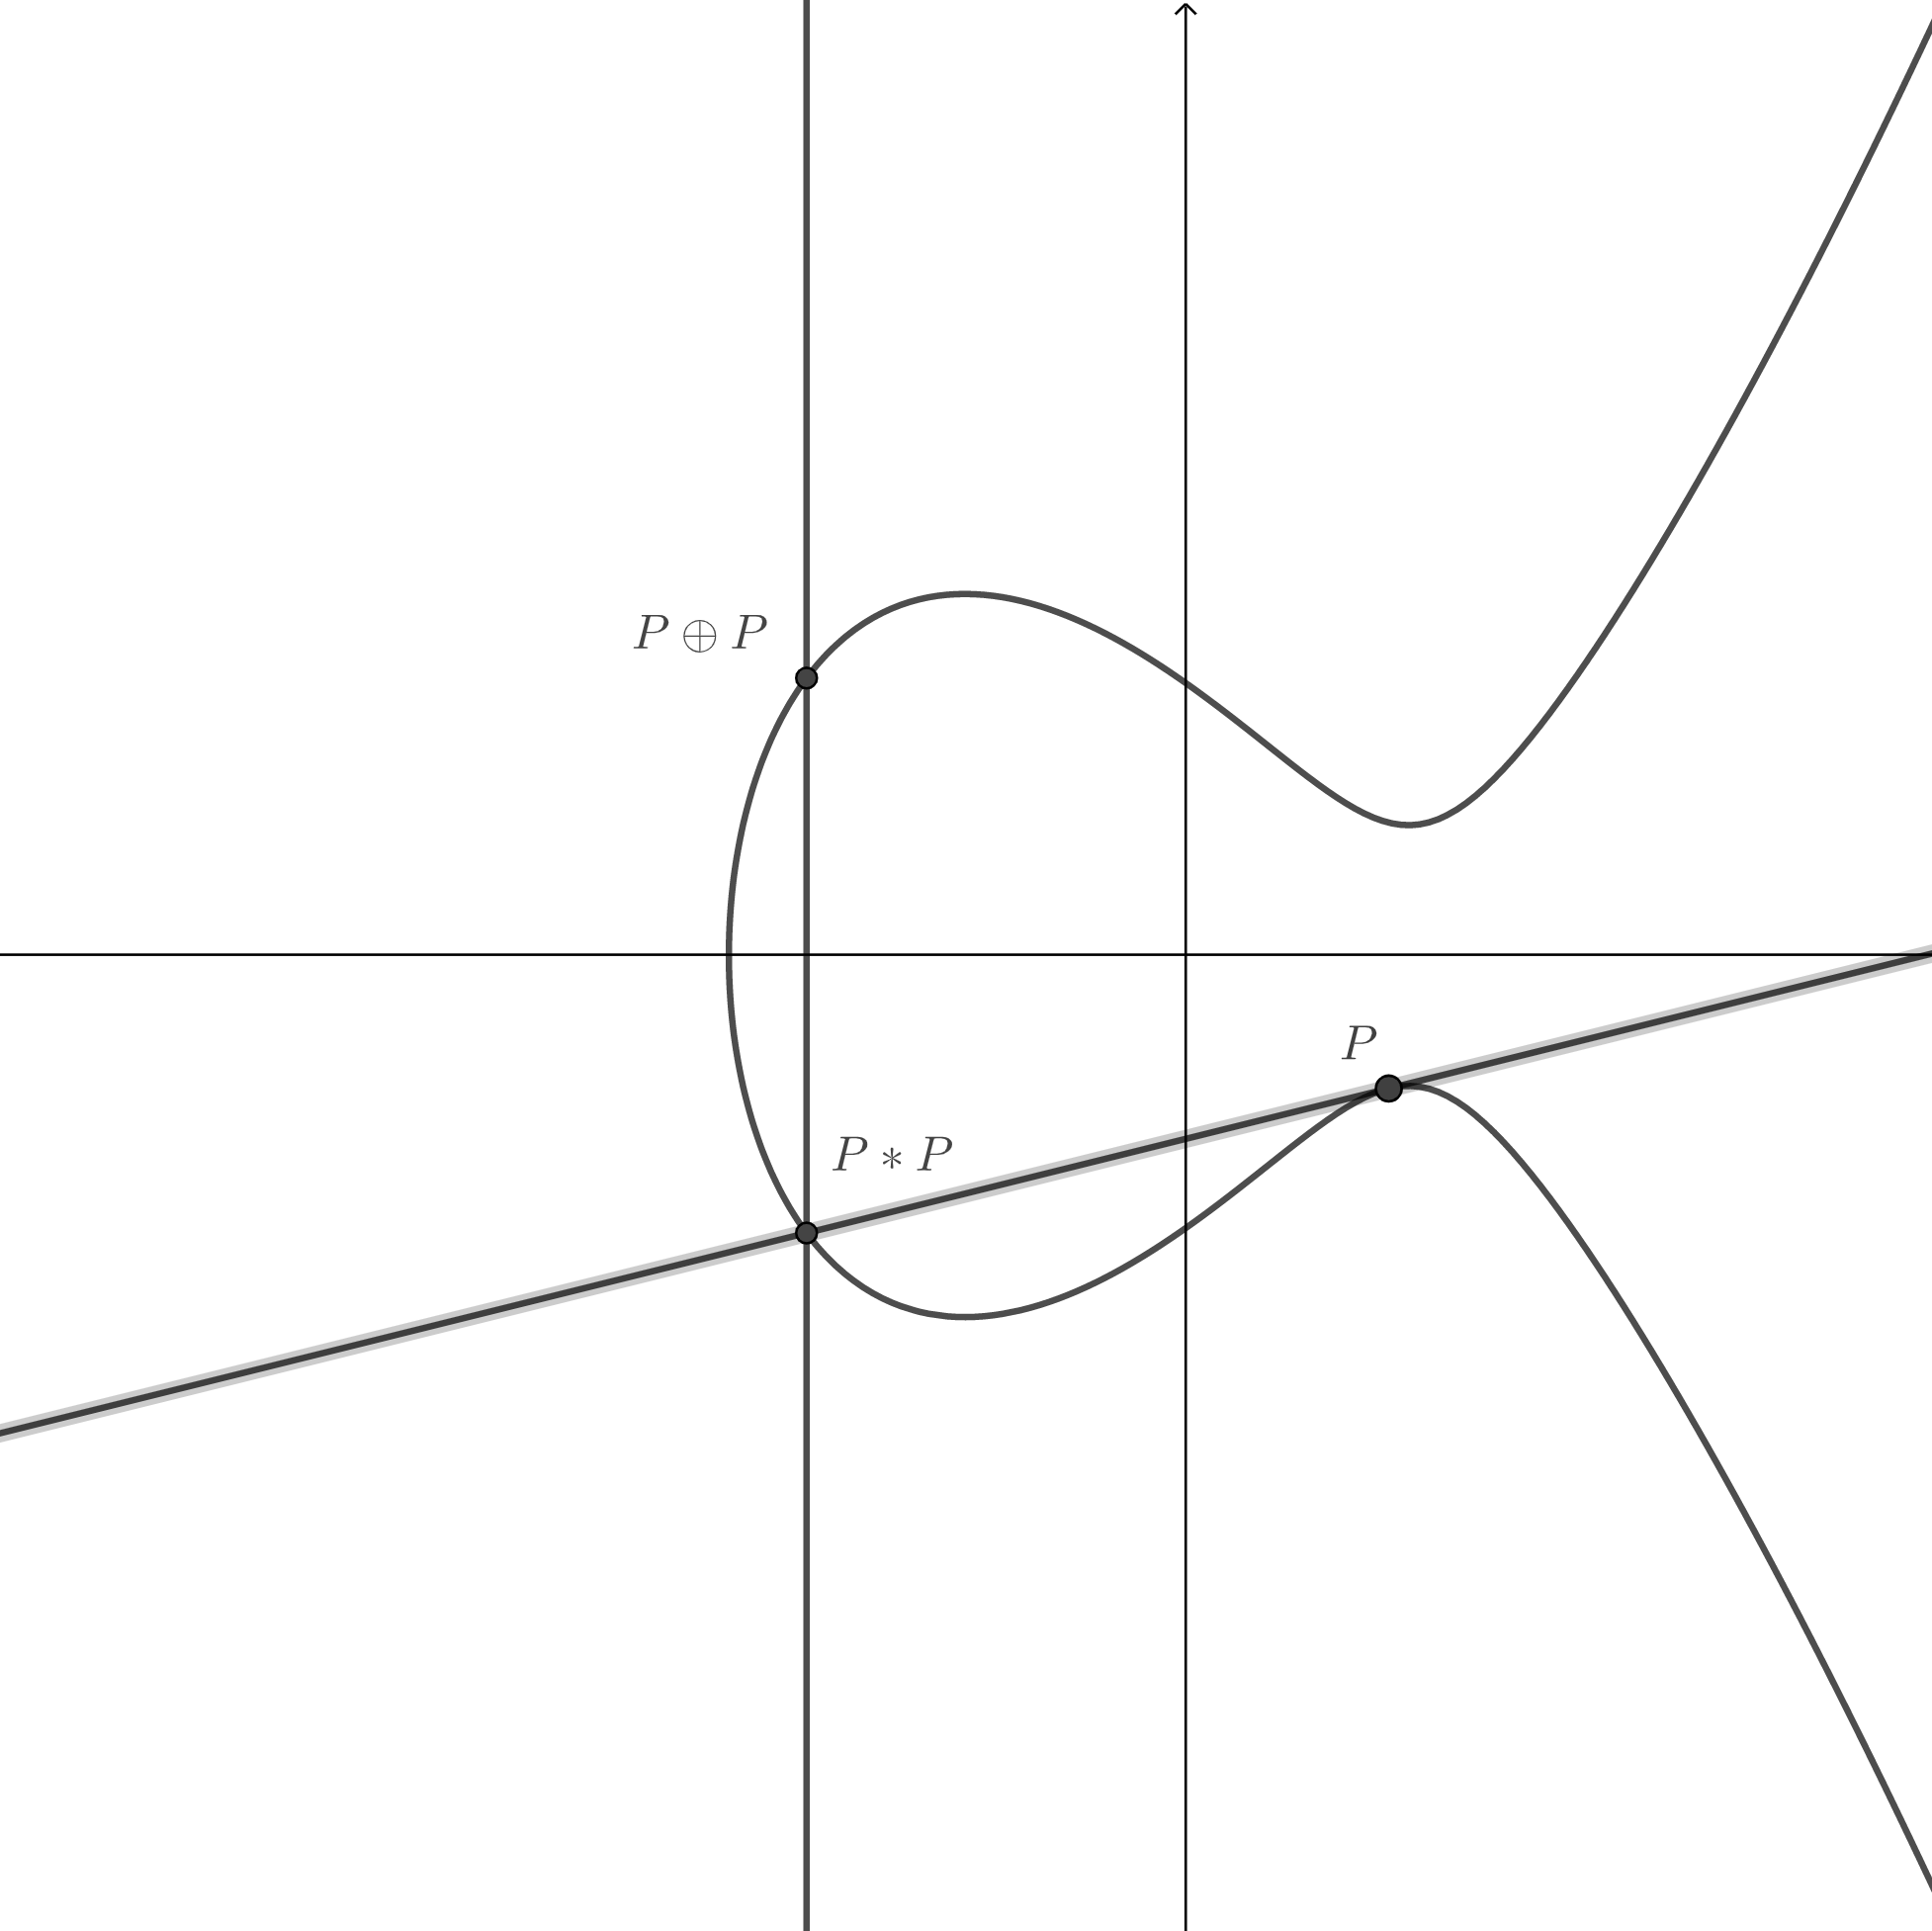
\includegraphics[width=.7\linewidth]{figures/2.png}
        \label{fig:sub2}
        \caption{$P\oplus P$}
        \end{subfigure}
        \end{figure}
        
        \begin{theorem}
            Suppose $E$ is an elliptic curve and $\oplus$ is the composition law defined above. Then $(E,\oplus)$ is an abelian group. If $E/k$, then $(E(k),\oplus)$ forms a subgroup. The composition law is therefore called the \textit{group law on $E$}, and we use $+$ instead of $\oplus$.
        \end{theorem}
        \begin{proof}
            The operation is commutative since the construction of $P*Q$ is symmetric. The existence of an identity is mentioned above. The inverse $-Q$ of $Q$ can be constructed by drawing a tangent line at $\mathcal{O}$, finding the third point of intersection $S$ with $E$, and finding the third point of intersection of the line joining $Q, S$ and the curve. The associativity is rather hard to prove. One may choose to argue geometrically, or simply writing down the explicit formulas.
        \end{proof}
        
    %%%%%%%% Subsection %%%%%%%%%%%%
    \subsection{Explicit formulas for the group law}
        Let $E$ be an elliptic curve defined by $$F(x, y)=y^2+a_1xy+a_3y-x^3-a_2x^2-a_4x-a_6.$$
    \begin{lemma}\label{lemma-explicit-neg}
        If $P_0=(x_0, y_0)\in E$, then $-P_0=(x_0, -y_0-a_1x_0-a_3)$.
    \end{lemma}
    \begin{proof}
        In order to calculate $-P_0$, we take the line $L$ through $P_0$ and $\ecO$ and finds its third point of intersection with $E$. The line $L$ is given by $$L:x-x_0=0.$$
        Substituting this into the equation for $E$, we see that $F(x_0,y)$ has two roots $y_0$ and $y_0'$, where $-P=(x_0,y_0')$. Writing out $$F(x_0,y)=c(y-y_0)(y-y_0')$$ and equating the coefficients of $y^2$ gives $c=1$, and similarly equating the coefficients of $y$ gives $y_0'=-y_0-a_1x_0-a_3$. This yields $$-P_0=(x_0, -y_0-a_1x_0-a_3).$$
    \end{proof}
    \begin{lemma}
        Let $P_1=(x_1,y_1)$ and $P_2=(x_2,y_2)$ be points on $E$. If $x_1=x_2$ and $y_1+y_2+a_1x_1+a_3=0$, then by \autoref{lemma-explicit-neg},
        $$P_1+P_2=\ecO.$$
        Otherwise define
        \[\lambda =
        \begin{cases}
            \frac{y_2-y_1}{x_2-x_1}, & x_1\neq x_2\\
            \frac{3x_1^2+2a_2x_1+a_4-a_1y_1}{2y_1+a_1x_1+a_3} , & x_1=x_2
        \end{cases},\quad\nu=\begin{cases}
            \frac{y_1x_2-y_2x_1}{x_2-x_1}, & x_1\neq x_2\\
            \frac{-x_1^3+a_4x_1+2a_6-a_3y_1}{2y_1+a_1x_1+a_3}, & x_1=x_2
        \end{cases}\]
        Then $y=\lambda x+\nu$ is the line through $P_1,P_2$ or tangent to $E$ if $P_1=P_2$.
    \end{lemma}
    \begin{proof}
        The proof of this lemma is trivial --- do some elementary computations!
    \end{proof}
    And we are ready to compute the addition formula of two points:
    \begin{lemma}
        Let $P_1=(x_1,y_1)$ and $P_2=(x_2,y_2)$ be points on $E$, and the equation through $P_1$ and $P_2$ (or the tangent line to $E$ if $P_1=P_2$) be $y=\lambda x+\nu $. Then we have that $$P_1+P_2=(\lambda ^2 +a_1\lambda -a_2-x_1-x_2,-(\lambda +a_1)x_3-\nu -a_3).$$
    \end{lemma}
    \begin{proof}
        Substituting the equation of $L$ into the equation of $E$, we see that $F(x,\lambda x+\nu )$ has roots $x_1,x_2,x_3$, where $P_3=(x_3,y_3)$ is the third point of $L\cap E$. We write out $$F(x,\lambda x+\nu )=c(x-x_1)(x-x_2)(x-x_3)$$ and equate coefficients. The coefficient of $x^3$ gives $c=-1$, and then the coefficient of $x^2$ gives $x_3=\lambda ^2 +a_1\lambda -a_2-x_1-x_2$. And substituting $x_3$ into the equation of $L$ gives the value of $y_3=\lambda x_3+\nu .$
    \end{proof}
    \begin{corollary}\label{corollary-dup-formula}
        When $P_1\neq P_2$, we have $$x(P_1+P_2)=\frac{y_2-y_1}{x_2-x_1}^2+a_1\frac{y_2-y_1}{x_2-x_1}-a_2-x_1-x_2,$$ and the \textup{duplication formula} for $P=(x,y)\in E$, $$x([2]P)=\frac{x^4-b_4x^2-2b_6x-b_8}{4x^3+b_2x^2+2b_4x+b_6},$$ where $b_2=a_1^2,b_4=2a_4+a_1a_3, b_6=a_3^2+4a_6$, and $ b_8=a_1^2a_6+4a_2a_6-a_1a_3a_4+a_2a_3^2-a_4^2.$
    \end{corollary}
    
    
    
    %%%%%%%% Subsection %%%%%%%%%%%%
    \subsection{Important invariants}
    $$E: y^2+a_1xy+a_3y=x+a_2x^2+a_4x+a_6,$$ and an extra point $O=[0,1,0]$ out at infinity.\\
    If $\text{char}(K)\neq 2$, we can simplify the equation into the form $$E: y^2=4x^3+b_2x^2+2b_4x+b_6,$$ where $$b_2=a_1^2+4a_4,\qquad b_4=2a_4+a_1a_3,\qquad  b_6=a_3^2+4a_6.$$
    We also define quantities:
    $$b_8=a_1^2a_6+4a_2a_6-a_1a_3a_4+a_2a_3^2-a_4^2,$$
    $$c_4=b_2^2-24b_4.$$
    \begin{definition}
        The quantity $\Delta$ is the discriminant of the Weierstrass equation, defined by $$\Delta =-b_2^2b_8-8b_4^3-27b_6^2+9b_2b_4b_6.$$ The $j$-invariant of the elliptic curve is given by $$j=c_4^3/\Delta .$$
    \end{definition}
    \begin{remark}
    Assuming that the characteristic of $K$ is not 2 or 3, take an elliptic curve and write it in Weierstrass form $$E: y^2=x^3+Ax+B.$$ 
    The discriminant of the Weierstrass equation is then given by $$\Delta = -16(4A^3+27B^2).$$
    And the $j$-invariant of the elliptic curve is given by $$j= -1728\frac{(4A)^3}{\Delta }.$$
    \end{remark}
    \begin{theorem}
        The curve given by a Weierstrass equation satisfies:
        \begin{enumerate}[\normalfont(i)]
            \item It is nonsingular if and only if $\Delta =0.$
            \item It has a node if and only if $\Delta =0$ and $c_4\neq 0.$
            \item It has a cusp if and only if $\Delta =c_4=0.$
        \end{enumerate}
        In cases (ii) and (iii), there is only the one singular point.
    \end{theorem}
    \begin{theorem}
        Two elliptic curves are isomorphic over $K$ if and only if they both have the same $j$-invariant.
    \end{theorem}
    \begin{proof}
        First, if two elliptic curves are isomorphic, then the transformation formulas show that they have the same $j$-invariant.\\
        For the converse, we will assume that $\text{char} (K)\geq 5.$ Let $E$ and $E'$ be the elliptic curves with the same $j$-invariant with the Weierstrass equations$$E: y^2=x^3+Ax+B,$$ $$E': y'^2=x'^3+A'x'+B'.$$
        Then by the assumption $j(E)=j(E')$, we have that $$\frac{(4A)^3}{4A^3+27B^2} = \frac{(4A')^3}{4A'^3+27B'^2},$$ which yields $$A^3B'^2=A'^3B^2$$
        In order to find an isomorphism of the form $(x,y)=(u^2x',u^3y')$, we consider three cases:
        \begin{enumerate}[\normalfont(i)]
            \item $A=0\ (j=0).$ Since $\Delta = -16(4A^3+27B^2)\neq 0$, $B\neq 0$, so $A'=0$. And we obtain an isomorphism using $u=(B/B')^{1/6}.$
            \item $B=0\ (j=1728).$ Then $A\neq 0$, so $B'=0$, and we take $u=(A/A')^{1/4}.$
            \item $AB\neq 0\ (j\neq 0,1728).$ If one of $A', B'$ were 0, then both of them would be 0, and $\Delta '$ would be 0, which is a contradiction. Therefore, $A'B'\neq 0$, and $u=(A/A')^{1/4}=(B/B')^{1/6}$ gives an isomorphism.  
        \end{enumerate}
    \end{proof}
    \begin{theorem}
        Let $j_0\in K.$ There exists an elliptic curve defined over $K(j_0)$ whose $j$-invariant is equal to $j_0$.
    \end{theorem}
    
    For consistency we define the \textit{invariant differential on an elliptic curve $E$} here: suppose $E;y^2+a_1y+a_3=x^2+a_2x^2+a_4x+a_6$, then the differential form
    \[\w=\frac{dx}{2y+a_1x+a_3}\]
    and we claim, without proof, that the invariant differential is regular and nonvanishing. The relevant terminologies will not be defined and used until \autoref{ssec-differential}





    %%%%%%%%%%%%%%%%%%%%%%%%%%%%%%%%%%%%%%%%%%%%%
    %%%%%%%%%%%%%%%% Section %%%%%%%%%%%%%%%%%%%%
    %%%%%%%%%%%%%%%%%%%%%%%%%%%%%%%%%%%%%%%%%%%%%
    \section{Elliptic Curves over $\mathbb Q$: Mordell-Weil Theorem}
        \textit{A brief introduction to the study of Elliptic Curves.}
        The study of Elliptic Curves could trace back to ancient Greece, when Diophantus of Alexandria, one of the great ancient mathematicians, formulated and solved many problems about the solution of polynomial equations in either integers or rational numbers, that is, the solution of
        $$F(x_1,\cdots,x_n)=0$$
        where $F$ is a polynomial in $n$ variables. The case of the polynomials in one variable is straightforward, as well as linear polynomials in two variables.
        
        The case of quadratic polynomials is solved by Hasse principle, namely:
        \begin{theorem}[Hasse principle]
            A homogeneous quadratic equation in several variables is solvable by integers, not all zero, if and only if it is solvable in real numbers and in $p$-adic numbers for each prime $p$.
        \end{theorem}
        
        Therefore the next easiest case would involve cubic polynomials in two variables. In this section, we present the Mordell's Theorem, a weaker version of the Mordell-Weil theorem: the group of rational points on a smooth cubic curve is finitely generated. We firstly need to define the height of a rational point on a smooth cubic curve $C:y^2 = x^3 + ax^2 + bx$. To start with, we define the \textit{height} of a rational point on the cubic $C$.
        
    %%%%%%%%%%%%%%%% subsection %%%%%%%%%%%%%%%%%%%%
    \subsection{Height of points}
         \begin{definition}
             Let $x=\frac{m}{n}$ be a rational number in lowest terms. The \textit{height} of $x$ is a positive number that defined to be the maximum of the absolute values of the numerator and the denominator of $x$.
             $$H(x)=H\left(\frac{m}{n}\right)=\max \{\lvert m \rvert,\lvert n \rvert\}.$$
         \end{definition}
         We can see the heights of rational points measure the complexity of rationals in a number-theoretic sense. Now consider an example:
         \begin{example}
            let $a = 1$, $b=\frac{999}{1000}$. These two rational numbers are very close to each other but there is a large difference in their heights.
         \end{example}
         \begin{definition}
             Let $P=(x,y)$ be a rational point on the curve $C$. The \textit{height} of $P$ is the height of its $x$-coordinate.
             $$H(P)=H(x)$$
             $H(\mathcal{O})$ is set to be $1$. We also define a \textit{``new" height} for rational points on elliptic curve by just taking the logarithm of heights which is more convenient for our further works
             $$h(P)=\log H(P)$$
         \end{definition}
         \begin{remark}
             It is easy to see that the set of all rational numbers whose height is less than some fixed number is a finite set. To see this, take $x=m/n < r$ in lowest terms for some real number $r$, then both $\lvert m \rvert,\lvert n \rvert < r$. Hence only finitely $m$ and $n$ in this set. Note that the set of all rational points on an elliptic curve also obeys the fact above. Indeed, for each of the possible $x$-coordinates of height less than $r$ there are at most two distinct $y$-coordinates for an elliptic curve. As the number of $x$-coordinates is finite, the number of points in this set is also finite. We conclude the discussion above with the following lemma:
         \end{remark}
         \begin{lemma}\label{lemma-bounded-height-fin}
             For every real number $r$, the set $\{ P\in C(\mathbb Q): h(P)<r \}$ is finite
         \end{lemma}
    \subsection{Bounding the heights}
        To prove Mordell's Theorem, more lemmas are needed, which we present below:
    
        \begin{lemma}\label{lemma-bound-h-add}
            Let $P_0$ be a fixed rational point of $C$. Then there is a constant $\kappa_0$ which depends on $P_0$, $a$, and $b$ such that
            $$h(P+P_0)\leqslant 2h(P) + \kappa_0$$
            for all $P\in C(\mathbb{Q})$.
        \end{lemma}

        In order to prove this lemma, we need to assume some results:
        \begin{lemma}\label{lemma-mordell-assump}
            Let $P = (x, y)$ be a rational point on $C$. Then
            \begin{enumerate}[\normalfont(i)]
                \item We can write $x$ and $y$ by $x = \frac{m}{d^2}, y = \frac{n}{d^3}$ for some integers $m,n,d$ with $d>0$ and $\gcd(m,d)=\gcd(n,d)=1$.
                \item There is some $K>0$ depending only on $a, b, C$ such that $\lvert m \rvert \leqslant H(P), \lvert d \rvert \leqslant H(P)^\frac{1}{2}, \lvert n \rvert \leqslant KH(P)^\frac{2}{3}$.
            \end{enumerate}
        \end{lemma}

        \begin{proof}
            Let $P = (x, y), P_0 = (x_0, y_0)$, and $P + P_0 = (x',y')$. Then $H(P+P_0) = H(x')$. Using the results from explicit formulas for the group law we can write $x'+x+x_0 = \lambda^2-a$ with $\lambda = \frac{y-y_0}{x-x_0}$. Proceed by rearranging
            \begin{align*}
                x' &= \left(\frac{y-y_0}{x-x_0}\right)^2 -a -x-x_0\\
                &=\frac{(y-y_0)^2-(a+x+x_0)(x-x_0)^2}{(x-x_0)^2}\\
                &=\frac{y^2-2yy_0+y_0^2-(a+x+x_0)(x-x_0)^2}{(x-x_0)^2}\\
                &=\frac{x^3+ax^2+bx-2yy_0+y_0^2-(a+x+x_0)(x-x_0)^2}{(x-x_0)^2}\\
                &=\frac{-2y_0y+x_0x^2+(b+2x_0a+x_0^2)x+(y_0^2+ax_0^2+x_0^3)}{x^2-2xx_0+x_0^2}\\
                &=\frac{Ay+Bx^2+Cx+D}{Ex^2+Fx+G}
            \end{align*}
            Where $\{A,B,..., G\}$ are rational numbers depending on $a,b,x_0,y_0$. Furthermore, we can multiply the expression by their least common denominator to assume $\{A,B,..., G\}$ are integers.

            By (i) in \autoref{lemma-mordell-assump}, we can write
            \begin{align*}
                x'&=\frac{A\frac{n}{d^3} + B\left(\frac{m}{d^2}\right)^2+ C\frac{m}{d^2}+D}{E\left(\frac{m}{d^2}\right)^2 +F\frac{m}{d^2}+G}=\frac{And+Bm+Cmd^2+Dd^4}{E+Fm^2+Gd^4}
            \end{align*}
            which means
            \[H(x') \leqslant \max \left\{| And+Bm+Cmd^2+Dd^4|, |E+Fm^2+Gd^4| \right\}\]

            Using (ii) in \autoref{lemma-mordell-assump}, there is some $K>0$ such that
            \begin{align*}
                \left| And+Bm+Cmd^2+Dd^4\right|& \leqslant |And| + |Bm| + |Cmd^2| + \lvert Dd^4 \rvert\\
                &\leqslant(\lvert AK \rvert + \lvert B \rvert + \lvert C \rvert + \lvert D \rvert)H(P)^2
            \end{align*}
            and
            \begin{align*}
                \lvert E+Fm^2+Gd^4 \rvert &\leqslant \lvert E \rvert + \lvert Fm^2 \rvert + \lvert Gd^4 \rvert\\
                &\leqslant  (\lvert E \rvert + \lvert F \rvert + \lvert G \rvert)H(P)^2
            \end{align*}
            Therefore $H(x') \leqslant \max \{ \lvert AK\rvert+\lvert B\rvert+\lvert C\rvert+\lvert D \rvert, \lvert E \rvert\ + \lvert F\rvert + \lvert G \rvert \}H(P)^2 $. Taking the logarithm, we get
            $$h(P+P_0)=\log H(x') \leqslant 2h(P) + \kappa_0$$
            where $\kappa_0 = \log \max \{ \lvert AK\rvert+\lvert B\rvert+\lvert C\rvert+\lvert D \rvert, \lvert E \rvert\ + \lvert F\rvert + \lvert G \rvert \} $ which only depends on $a,b,x_0,y_0$, completing the proof.
        \end{proof}
        \begin{remark}
            The proof above does not apply if $P = P_0, -P_0,\mathcal{O}$. For $P=\mathcal{O}$, the result is trivial, and the other two cases can be avoided using the duplication formula. The inequality still holds because for finitely many $P$, we can simply look at the differences $h(P + P_0) - 2h(P)$ and take $\kappa_0$ larger than the finite number of values that occur.
        \end{remark}
        \begin{lemma}\label{lemma-bound-4h}
            There is a constant $\kappa$, depending on $a$ and $b$, that
            $$h(2P)\geqslant 4h(P)-\kappa$$
            for all $P\in C(\mathbb{Q})$.
        \end{lemma}
        We still need some extra results for proving this lemma. Proofs are omitted as they are not especially related to elliptic curves.
        \begin{lemma}\label{lemma_mordell_assump2}
        let $\phi(X),\psi(X)$ be polynomials with integer coefficients and no common complex roots. Let $d$ be the maximum of the degrees of $\phi$ and $\psi$.
        \begin{enumerate}[\normalfont(i)]
             \item There is an integer $R \geq 1$, depending on  $\phi$ and $\psi$, so that for all rational numbers $m/n$
             $$\gcd\left(n^d\phi\left(\frac{m}{n}\right),n^d\psi\left(\frac{m}{n}\right)\right)$$ divides $R$
             
             \item There are constants $\kappa_1,\kappa_2$, depending on $\phi$ and $\psi$, so that for all for for all rational numbers $m/n$ which are not roots of $\psi$
             $$dh\left(\frac{m}{n}\right)-\kappa_1 \leqslant h\left(\frac{\phi\left(\frac{m}{n}\right)}{\psi\left(\frac{m}{n}\right)}\right) \leqslant dh\left(\frac{m}{n}\right)+\kappa_2$$
        \end{enumerate}
        \end{lemma}
        By using the results above, we are now ready to give a proof of \autoref{lemma-bound-4h}.
        
        \begin{proof}
            Similar as the case of \autoref{lemma-bound-h-add},ignoring a finite set of points would not affect the inequality. So it is reasonable to discard the finite many points such  $2P=\mathcal{O}$. We will see the reason to exclude these points later.\\
            Now assume $P=(x,y), 2P=(x',y')$. Duplication formula applied here:\\
            $x'+2x=\lambda^2 -a$ with $\lambda = \frac{f^\prime (x)}{2y}$. Proceed by rearranging. Note $y^2 = f(x) = x^3+ax^2+bx$ here. Thus,
            \begin{align*}
                 x' &= \left(\frac{f^\prime (x)}{2y}\right)^2-2x-a\\
                 &= \frac{f^\prime (x)^2}{4y^2}-(a+2x)\\
                 &= \frac{f^\prime (x)^2-(4a+8x)f(x)}{4f(x)}\
                 &= \frac{(3x^2+2ax+b)^2-(4a+8x)(x^3+ax^2+bx)}{4(x^3+ax^2+bx)}\\
                 &= \frac{x^4-2bx^2+b^2}{4x^3+4ax^2+4bx}
            \end{align*}
            where the third equality holds because $f(x)\neq 0$ if and only if $2P \neq \mathcal{O}$. Hence $x‘$ is a quotient of two polynomials in $x$ with integer coefficients, due to the fact that $f(x)$ is non-singular from assumption, we know that $f(x)$ and $f^\prime (x)$ have no common complex roots. It follows that the polynomials in the numerator and denominator of $x'$ also have no common roots. Since $h(P)=h(x),h(2P)=h(x')$ , it is suffice to show $h(x') \geqslant 4h(x)-\kappa$ for this lemma. As and the maximum degree of the polynomials in the numerator and denominator is $4$. This inequality could be derived by \autoref{lemma_mordell_assump2} (ii) as the maximum degree of the polynomials in the numerator and denominator is $4$ and $h(x)=h(m/n)$. Together with the fact that the polynomials in the numerator and denominator of $x'$ depend on $a, b$, finishing the proof.
            
        \end{proof}
        
        \begin{lemma}\label{lemma-fin-ind}
            The index
            $$[C(\mathbb{Q}):2C(\mathbb{Q})]$$
            is finite, where $2C(\mathbb{Q})$ is the set of rational points $Q$ that are equal to $P + P$, where $P$ is a rational point on $C(\mathbb{Q})$.
        \end{lemma}
        
        We give an outline for the proof. For the curve $C:y^2=x^3+ax^2+bx$, define $\bar{a}=-2a,\bar b=a^2-4b$.
        This gives a new curve $\bar C:y^2=x^3-2ax^2+(a^2-4b)x$.
        
        These two curves are closely related. To see this, define the function $\phi: C\rightarrow\bar C$:
        $$(x,y)\rightarrow(\bar x,\bar y):=(\frac{y^2}{x^2},y\frac{x^2-b}{x^2}),$$
        one could easily show this new point $(\bar x,\bar y)$ is indeed a rational point on $\bar C$.
        Similarly, define $\bar\phi: \bar C\rightarrow\bar{\bar C}$:
        $$(\bar x,\bar y)\rightarrow(\bar{\bar x},\bar{\bar y}):=(\frac{{\bar y}^2}{{\bar x}^2},{\bar y}\frac{{\bar x}^2-b}{{\bar x}^2}),$$
        then the composition of functions $\bar\phi\circ\phi$, gives exactly the endomorphism $C(\mathbb Q)\rightarrow C(\mathbb Q):P\rightarrow 2P.$
        In specific, both the index $(C(\mathbb Q):\phi(C(\mathbb Q)))$ and $(\phi(C(\mathbb Q)):\bar\phi(C(\mathbb Q)))$ are finite, so as their composition, the index $(C(\mathbb Q):2C(\mathbb Q))$ is also finite.
        
        We would not give a complete proof of \autoref{lemma-fin-ind} for similar reasons as \autoref{lemma_mordell_assump2} and \autoref{lemma-mordell-assump}. You can find detailed information of them in \cite{silverman_2015_rational}.
        
        
    %%%%%%%%%%%%%%%% subsection %%%%%%%%%%%%%%%%%%%%
    \subsection{A proof due to Mordell}
        Mordell presented a proof in 1922 of his theorem concerning the rational points on a cubic curve \cite{mordell1}. A revised proof in modern languages is reproduced below.
        \begin{theorem}[Mordell's Theorem]
            Let $C$ be a smooth cubic curve given by some equation
            $$C:y^2 = x^3 + ax^2 + bx$$
            where $a$ and $b$ are integers, then the rational points on $C$ form a group $C(\mathbb{Q})$, and $C(\mathbb{Q})$ is finitely generated.
        \end{theorem}
    
        \begin{proof}
            We start with \autoref{lemma-fin-ind} that the index $[C(\mathbb{Q}):2C(\mathbb{Q})]$ is finite. We can assume that $$C(\mathbb{Q})=\bigsqcup_{k=1}^n\left[Q_k+2C(\mathbb{Q})\right]$$
            for some rational points $Q_1,\dots,Q_n$. Thus any point $P_0\in C(\mathbb{Q})$ could be written in the form
            $$P_0 = Q_{n_1}+2P_1$$
            for some rational point $P_1$.
            Repeating this process for $P_1$ and subsequently for each $P_i$, we obtain
            $$P_i = Q_{n_{i+1}}+2P_{i+1}$$
            for all $0\leqslant i\leqslant m-1$. Combining these results we get:
            \begin{align*}
                P_0 &= Q_{n_1}+2P_1\\
                &= Q_{n_1}+2Q_{n_2}+4P_2\\
                &= Q_{n_1}+2Q_{n_2}+4Q_{n_3}+8P_3\\
                &=\cdots\\
                &= Q_{n_1}+2Q_{n_2}+4Q_{n_3}+\cdots+2^{m-1}Q_{n_m}+2^mP_m
            \end{align*}
    
        This pattern can repeat forever if needed. The above formula thus indicates that this specific point $P$ is generated by the representatives $Q_1,\cdots,Q_n$ and $P_m$, but the problem is that $P_m$ depends on $P$. However, it would be nice if we could show that there are only finitely many possible $P_m$,  say $P_{m_1},\cdots,P_{m_s}$, no matter which $P$ we choose, because then every point $P\in C(\mathbb{Q})$ could be written as
        $$P = 2^{m_j}P_{m_j}+\Sigma_{i=0}^{m_j}a_iQ_{n_i}$$
        for some $P_{m_j}\in \{P_{m_1},\cdots,P_{m_s}\}$.
    
        Notice that it is sufficient to prove that the heights of $P_{m_1},\cdots,P_{m_s}$ are bounded by some real number $M$: there are only finitely positive integers less or equal than $M$, so there are at most $2M^2$ rational points with height no more than $M$. In particular, this is a finite set of points.
    
        Following this strategy, we now show that all possible $P_m$'s have their height bounded by a certain real number $M$, by choosing a sufficiently large $m$. Applying \autoref{lemma-bound-h-add} to $P_m$ and $-Q_1,\cdots,-Q_n$, one obtains constants $\kp_i$ such that
        $$h(P_m-Q_i)\leqslant 2h(P_m) + \kappa_i.$$
        Let $\kappa_{\max}=\max(\kappa_i)$. We get
        $$h(P_m-Q_i)\leqslant 2h(P_m) + \kappa_{\max}$$
        for all $i$. By \autoref{lemma-bound-4h}, applied to $P_m$,
        $$4h(P_m)\leqslant h(2P_m)+\kappa=h(P_{m-1}-Q_{n_m})+\kappa\leqslant 2h(P_{m-1}) + \kappa_{\max}+\kappa$$
        In the equation we used $P_{m-1} = Q_{n_m}+2P_m$.
    
        Dividing both sides by four gives
        $$h(P_m)\leqslant \frac{h(P_{m-1})}{2}+\frac{\kappa_{\max}+\kappa}{4}=\frac{3}{4}h(P_{m-1})+\frac{\kappa_{max}+\kappa-h(P_{m-1})}{4}.$$
    
        Now we set $M=\kappa_{max}+\kappa$, and show that $h(P_m)\leq M$ for a sufficiently large $m$. If $h(P_{m-1})\leqslant \kappa_{\max}+\kappa$, then we are done. Otherwise we have $h(P_{m-1})> \kappa_{\max}+\kappa$, which means 
        $$h(P_m)\leqslant\frac{3}{4}h(P_{m-1})+\frac{\kappa_{max}+\kappa-h(P_{m-1})}{4}<\frac{3}{4}h(P_{m-1}).$$
        Since $3/4<1$, it is guaranteed that $h(P_m)\rightarrow 0$ as $m\to\infty$. In particular, for a sufficiently large $m$, $h(P_m)\leq \kappa_{max}+\kappa=M$.
    
        We thus showed for any $P = 2^mP_m+\Sigma_{i=0}^ma_iQ_{n_i}$, and a sufficiently large $m$, the height of $P_m$ is no more than $M$. Together with \autoref{lemma-bounded-height-fin}, we've shown that there are only finitely many possible $P_m$'s. Thus, any point $P\in C(\mathbb{Q})$ is (finitely) generated by
        $$\{Q_1,\cdots,Q_n\}\cup\{\text{finitely many possible }P_m\},$$
        completing the proof.
    \end{proof}
    
    
    
    %%%%%%%%%%%%%%%%%%%%%%%%%%%%%%%%%%%%%%%%%%%%%
    %%%%%%%%%%%%%%%% Section %%%%%%%%%%%%%%%%%%%%
    %%%%%%%%%%%%%%%%%%%%%%%%%%%%%%%%%%%%%%%%%%%%%
    \newpage
    \section{More on Curves}
    %%%%%%%%%%%%%%%% subsection %%%%%%%%%%%%%%%%%%%%
	\subsection{Curves and rational points}\label{sec-rat}
        We require all varieties in this report to be irreducible.
        \begin{definition}\label{def-curve}
            A \textit{curve} is a projective variety of dimension $1$.
        \end{definition}
        \noindent Therefore, we are only interested in projective varieties and most of the objects will be constructed in them. In order to study the rational solutions of a certain type of equations (that is, on some curves), it is important to base all geometric constructions on some algebraically closed extension of the field we are interested in. Say $k$ is a perfect field and $K$ an algebraic closure of $k$, we denote by $\Gal(K/k)$ the Galois group of $K/k$ (the fixed field of this group is $k$ as $K$ is an algebraic, separable and normal extension of $k$). We can define a natural group action of $\Gal(K/k)$ on the projective space $\mathbb P^n$ over $K$ by $[x_0:\cdots: x_n]^\sigma =[x_0^\sigma:\cdots: x_n^\sigma]$ for any $\sigma$ in the Galois group. We introduce the following notations/definitions.
        \begin{definition}
            The \textit{set of $k$-rational points} $\mathbb P^n(k)$ is the set $\{[x_0:\cdots:x_n]: \forall i, x_i\in k\}$. Given a projective variety $V$, the \textit{$k$-rational points of $V$} is the set $V(k)=V\cap \mathbb P^n(k)$.
        \end{definition}
        \begin{definition}
            A projective variety $V$ is said to be \textit{defined over $k$}, written as $V/k$, if $\mathbb I(V)$ can be generated by homogeneous polynomials with rational coefficients (i.e., in $k[x_0,\dots, x_n]$).
        \end{definition}
        \begin{remark}
            We can also use Galois-theoretic languages:
            \[\mathbb P^n(k)=\{P\in \mathbb P^n:P^\s = P,\forall\s \in\Gal(K/k)\},\]
            and
            \[V(k)=\{P\in V:P^\s = P,\forall\s \in\Gal(K/k)\}\]
            as the fixed field of the Galois group is $k$.
        \end{remark}
        Since we are working with low dimensional cases, it is convenient to define the function field of a projective variety using an affine chart. For any variety $W$ we define 
        \[k[W]=k[x_0,\dots,x_n]/\mathbb I(W/k)\]
        where $\mathbb I(W/k)=\mathbb I(W)\cap k[x_0,\dots,x_n]$.
        \begin{definition}
            Given a projective variety $V/k$, choose some $U_i=\{x_i\neq 0\}\subseteq \mathbb P^n$. Define the \textit{function field of $V$}, $k(V)$, to be the quotient field of $k[V\cap U_i]$ and the \textit{larger function field of $V$} to be the quotient field of $K[V\cap U_i]$.
        \end{definition}
        \begin{remark}
            The choice of the chart does not matter --- the resulting fields are isomorphic. The elements in $K(V)$ are of the form $f/g$ where $f, g$ are homogeneous polynomials of the same degree in $n+1$ variables, $g\notin\mathbb I(V)$.
        \end{remark}
        For some projective variety $V$, we can define a group action of $\Gal(K/k)$ on $K[V]$ sending $f=\sum a_{I}x^I$ to $f^\s=\sum \s(a_I)x^I$, that is, acting on the coefficients of $f$. We can further extend this group action to $K(V)$ by defining $(f/g)^\s=f^\s/g^\s$. It is easy to check that the invariant sets in $K[V]$ and $K(V)$ are $k[V]$ and $k(V)$ respectively.
        \begin{remark}\label{remark-gal-on-rational}
            Since $\Gal(K/k)$ consists of field endomorphisms, we have $(f(P))^\s=f^\s(P^\s)$ for all $f$ and points $P$.
        \end{remark}
        
        Suppose $V_1, V_2$ are two projective varieties. For any rational map $\varphi=[f_0:\cdots:f_n]:V_1\to V_2$ where $f_i\in K(V_1)$, we define a group action $\varphi^\s=[f_0^\s:\cdots:f_n^\s]$. And by \autoref{remark-gal-on-rational}, we get $(\varphi(P))^\s=\varphi^\s(P^\s)$.
        \begin{definition}
            A rational map $\varphi=[f_0:\cdots:f_n]$ on $V$ is \textit{defined over $k$} if there exists some nonzero $\lambda\in K$ such that $\lambda f_i\in k(V)$ for all $i$. Equivalently, $\varphi^\s=\varphi$ for all $\s\in\Gal(K/k)$.
        \end{definition}
        \begin{definition}
            For any projective variety $V$ and a smooth point $P\in V$, the maximal ideal at $P$ is $\mathfrak m_P=\{f\in K[V]:f(P)=0\}$. The \textit{local ring of $V$ at $P$}, denoted by $K[V]_P$ is the localization $K[V]_{\mathfrak m_P}$ which is simply the local ring
            \[K[V]_P=\{f/g:f, g\in K[V]\text{ and } g(P)\neq 0\}\]
            A rational function $f\in K(V)$ is said to be regular at $P$ if $f\in K[V]_P$.
        \end{definition}
        \noindent These definitions are equivalent to the mostly seen ones, but it would require some nontrivial arguments to prove the equivalence. See \cite{hartshorne_2010_algebraic} for instance. They also allow us to do most of our explicit computations on affine coordinate rings, while using the projective varieties to make certain huge theorems work.
        \begin{remark}
            Since for a projective variety $V$ the closure of $V\cap \A^n$ in $\Pc^n$ is simply $V$, we will always use the affine variety to represent $V$ and other objects on $V$.
        \end{remark}
        
        
        
        
    %%%%%%%% Subsection %%%%%%%%%%%%
    \subsection{Local rings at smooth points}
        We reproduce \autoref{def-curve} below.
        \begin{definition}
            A \textit{curve} is a projective variety of dimension $1$.
        \end{definition}
        In our report, the term curve refers to \textbf{smooth} curves, which are curves with all points smooth. Standard algebraic geometry results show that if $P$ is a smooth point of a projective variety $V$, then the dimension (over $K$) of $\mathfrak m_P/\mathfrak m_P^2$ (\cite{hartshorne_2010_algebraic}) equals the dimension of $V$. Thus, given any curve $C$, we have $\dim_K \mathfrak m_P/\mathfrak m_P^2=1$, which gives us the following commutative algebra result:
        \begin{lemma}\label{lemma-ord}
            For all points $P$ in the curve $C$, the local ring $K[C]_P$ is a discrete valuation ring with a valuation defined by
            \[\ord_P(f)=\sup\{d\in\N:f\in\mathfrak m_P^d\}\]
            which is a map $K[C]_P\to\N\cup\{\infty\}$. Furthermore, each valuation $\ord_P$ can be extended to $K(C)$ by $\ord_P(f/g)=\ord_P(f/1)-\ord_P(g/1)$. This map is called \textup{the order of $f/g$ at $P$}.
        \end{lemma}
        \begin{proof}
            Prop. 9.2 in \cite{atiyah1994introduction}.
        \end{proof}
        \begin{remark}
            The fraction field of a localization of some ring is isomorphic to the fraction field of the original ring. Therefore, $K(C)$ is the fraction field of $K[C]_P$ for any $P$.
        \end{remark}
        \begin{definition}
            The \textit{uniformizer for $C$ at $P$} is some element $t\in K(C)$ such that $\ord_P(t)=1$.
        \end{definition}
        \begin{remark}\label{remark-unif-exist}
            There certainly exists a uniformizer: since every discrete valuation ring is a principal ideal domain, $\mathfrak m_P=(t)$ for some $t$, which must be of order one as suggested by commutative algebra results.

            If $t\in K(C)$ is of order one, then for any $g\in\mathfrak m_P$ (meaning $\ord_P(g)\geqslant 1$), we have
            \[\ord_P(g/t)=\ord_P (g)-1\geqslant 0\]
            so $g/t\in K[C]_P$, meaning there exists some $h\in K[C]_P$ such that $g=th$ and thus $\mathfrak m_P=(t)$.
        \end{remark}
        \noindent To assist further understandings of this valuation, we present the following example.
        \begin{example}
            Consider the curve $y^2=x^3+2x$ over a field $K$ with characteristic not equal to $2$, which is smooth. Let $P=(0, 0)$ then $\mathfrak m_P=(x, y)$ and $\mathfrak m_P^2=(x^2,xy,y^2)$. Since $x=\frac{1}{2}(y^2-x^3)\in\mathfrak m_P^2$ (this also tells us $\ord_P(x)\geqslant 2$), $\mathfrak m_P=(x, y)=(y)$ (in the local ring at $P$). Thus, $\ord_P(y)=1$. Now $y^2=(x^2+2)x$ where $x^2+2\neq 0$ at $P$ which means it's a unit in the local ring, $x=(x^2+2)^{-1}y^2$ and thus
            \[\ord_P(x)=\ord_P(\text{some unit})+2\ord_P(y)=2\]
            where the order of unit must be zero by definition (otherwise $\mathfrak m_P$ wouldn't be maximal). Finally for $2y^2-3x=2x^3+x=(2x^2+1)x$, we have
            \[\ord_P(2y^2-3x)=\ord_P(\text{some unit})+\ord_P(x)=2\]
            where the equality holds since $2x^2+1\neq 0$ at $P=(0, 0)$, i.e., $2x^2+1$ is a unit.
        \end{example}
        Let $k$ be a field of characteristic $p>0$.
        \begin{lemma}\label{lemma-unif-sep}
            Given curve $C/k$ and $t\in k(C)$ a uniformizer at a smooth $P\in C(k)$. Then $k(C)$ is a finite separable extension of $k(t)$.
        \end{lemma}
        \begin{proof}
            Since $k(C)$ is a finitely generated $k$-algebra, Zaraski's lemma ensures it's a finite extension of $k$. Clearly $k(t)$ has transcendence degree $1$ ($t\notin k$ otherwise $\ord_P t=0$ for all $P\in C$). Now as the transcendence degree of $k(C)/k$ is $\dim C=1$, $\trdeg k(C)/k(t)=0$, meaning $k(C)$ is an algebraic extension of $k(t)$.

            Take any $x\in k(C)$ and we aim to show $x$ is separable over $k(t)$. Since $k(C)$ is algebraic, there is some $\Phi(X, T)\in k[X, T]$ such that $\Phi(x, t)=0$. Suppose further that $\Phi$ has minimal degree over $k(t)$.

            If there is some term $a_{ij}T^iX^j$ in $\Phi$ where $p\nmid j$, then clearly $\partial\Phi(t, X)/\partial X$ is nonzero, meaning $x$ is separable.

            It remains to check when $\Phi(T, X)=\Psi(T, X^P)$ for some polynomial $\Psi$. Write
            \[\Phi=\Psi(T, X^p)=\sum_{k=0}^{p-1}\left(\sum_{i,j}b_{ijk}T^{ip}X^{jp}\right)T^k\]
            Since $k$ is perfect of characteristic $p>0$, every element of $k$ is a $p$th power. Thus, define $c_{ijk}^p=b_{ijk}$ and thus
            \[\sum_{i,j}b_{ijk}T^{ip}X^{jp}=\sum_{i,j}(c_{ijk}X^iT^j)^p=\left(\sum_{i,j}c_{ijk}X^iT^j\right)^p=\varphi_k(T, X)^p\]
            
            Evaluate the order of each summand:
            \[\ord_P(\varphi_k(t, x)^pt^k)=p\ord_P(\cdots)+k\ord_P(t)\equiv k\pmod{p}\]
            which means they have different orders, and thus must all vanish as $\Phi(t, x)=0$. There must exist some $k$ such that $\varphi_k$ contains $X$ and $\varphi_k(t, x)=0$. Yet $\Phi(t, X)$ is minimal and $\deg \varphi_k(t, X)^p\leqslant \deg \Phi(t, X)$ so we get a contradiction.
        \end{proof}

        \begin{definition}
            For any point $P$ on a curve $C$ and any $f\in K(C)$, if $\ord_P(f)\geqslant 0$ then $f$ is \textit{regular at $P$}. If $\ord_P(f)>0$ then $f$ has \textit{a zero of order $\ord_P(f)$ at $P$}; if $\ord_P(f)<0$ then $f$ has \textit{a pole of order $-\ord_P(f)$ at $P$}
        \end{definition}
        \begin{remark}
            If $f=g/h$ is regular at $P$, then $f$ corresponds to some element of $K[C]_P$, meaning there exist $g',h'\in K[C]$ such that $h'\neq 0$ near $P$ and thus $f$ is regular at $P$ in the usual sense.
        \end{remark}
        The order $\ord_P$ at any point $P$ satisfies a very important property, which is an essential part of our algebraic geometry machine.
        \begin{theorem}\label{theorem-fin-ord}
            Let $C$ be a curve and $f\in K(C)$. Then the set $\{P\in C:\ord_P(f)\neq 0\}$ is finite. Furthermore, if $f$ has no poles on $C$, then $f\in K$.
        \end{theorem}
        \begin{proof}
            The proof of this theorem by elementary variety theory is rather long and complicated. A short proof using schemes is available in \cite{hartshorne_2010_algebraic}, II.6.1.
        \end{proof}
        
        
        
    %%%%%%%% Subsection %%%%%%%%%%%%
    \subsection{Morphisms of curves}
        Let $C_1, C_2$ be two (smooth) curves. A rational map $\varphi: C_1\to C_2$ is a morphism if it's regular at every point on $C_1$. We present a small lemma as an application of $\ord$. The term regular 
        \begin{lemma}
            Any rational map $\varphi=[f_0:\cdots:f_m]:C\to V$ from a (smooth) curve to a variety $V\subseteq \mathbb P^m$ is a morphism.
        \end{lemma}
        \begin{proof}
            It suffices to show that for all $P\in C$, there is some $g\in K(C)$ such that each $gf_i$ is regular at $P$. Let $m=\min_{i}\ord_P(f_i)$. As \autoref{remark-unif-exist} suggests, there is a uniformizer at $P$, say $t$, such that $\ord_P(t)=1$. Then $\ord_P( t^{-m}f_i)\geqslant 0$ for all $i$, completing the proof.
        \end{proof}
        If $C_1/k$ and $C_2/k$, a nonconstant rational map $\varphi:C_1\to C_2$ defined over $k$ induces an injective pullback $\varphi^*:k(C_2)\to k(C_1)$ fixing $k$. We quote the following theorem:
        \begin{theorem}\label{theorem-map-fin}
            Given curves $C_1/k$ and $C_2/k$, the following statements hold:
            \begin{enumerate}[\normalfont(i)]
                \item For any nonconstant rational map $\varphi$, $k(C_1)$ is a finite extension of the pullback of $k(C_2)$, that is, $[k(C_1):\varphi^*k(C_2)]<\infty$.
                \item For any injective field homomorphism $\psi:k(C_2)\to k(C_1)$ fixing $k$, there is a nonconstant rational map $\varphi:C_1\to C_2$ such that $\varphi^*=\psi$.
            \end{enumerate}
        \end{theorem}
        \begin{proof}
            The proof is omitted.
        \end{proof}
        \begin{definition}
            Suppose $\varphi:C_1\to C_2$ is a rational map. If $\varphi$ is constant we define the \textit{degree of $\varphi$}, $\deg\varphi$, to be $0$ and if $\varphi$ is nonconstant, then we define
            \[\deg\varphi=[k(C_1):\varphi^*k(C_2)]\]
            In particular, a rational map $\varphi$ is \textit{separable, inseparable or purely inseparable} if the extension $k(C_1)/\varphi^*k(C_2)$ is (see definitions in \autoref{ssec-fields}).
        \end{definition}
        \begin{definition}
            We define the \textit{ramification index of $\varphi$ at $P$} to be the order
            \[e_\varphi(P)=\ord_P\left(\varphi^*t_{\varphi(P)}\right)\]
            where $t_{\varphi(P)}$ is any uniformizer at $\varphi(P)$. Note: the choice of $t$ does not matter.
        \end{definition}
        Here are some general facts about the ramification index:
        \begin{lemma}\label{lemma-rami}
            Suppose $\varphi:C_1\to C_2$ is a nonconstant morphism, then
            \begin{enumerate}[\normalfont(i)]
                \item For all $Q\in C_2$,
                \[\sum_{P\in\varphi^{-1}(Q)}e_{\varphi}(P)=\deg \varphi\]
                \item For all but finitely many $Q\in C_2$,
                \[\#\varphi^{-1}(Q)=\deg_s \varphi\]
                where $\deg_s$ is the separable degree
                \[[\varphi^*k(C_2)^{\mathrm{sep}}:\varphi^*k(C_2)]\]
                from \autoref{theorem-sep-exist}
            \end{enumerate}
            Furthermore, if $\psi:C_2\to C_3$ is another nonconstant map,
            \[e_{\psi\circ\varphi}(P)=e_{\psi}(\varphi(P))e_{\varphi}(P)\]
        \end{lemma}
        \begin{proof}
            The first two statements are nontrivial and can be found in \cite{hartshorne_2010_algebraic}.
            
            For the last statement, let $t_1,t_2$ be uniformizers at at $\varphi(P)$ and $\psi(\varphi(P))$ respectively. Then by definition
            \[\ord_{\varphi(P)}\left(t_1^{e_{\psi}(\varphi(P))}\right)=e_{\psi}(\varphi(P))=\ord_{\varphi(P)}(\psi^*t_2)\]
            and thus,
            \[e_{\varphi\circ\varphi}(P)=\ord_{P}((\psi\circ\varphi)^*t_2)=\ord_{\varphi(P)}(\varphi^*t_1^{e_{\psi}(\varphi(P))})=e_{\psi}(\varphi(P))e_{\varphi}(P)\]
            which completes the proof.
        \end{proof}
    \subsection{The Frobenius map}
        On a field $K$ of characteristic $p>0$, we have an extremely important map --- \textit{the Frobenius endomorphism} $F:x\mapsto x^p$. It is clear that $F(x+y)=F(x)+F(y)$ since the prime $p$ divides all $\binom{p}{k}$ with $0<k<p$.
        \begin{remark}
            The invariant set of the $n$th iterate of the Frobenius endomorphism (that is, $F^n$) is simply $\F_{p^n}$. This property is one of the most essential ``reasons" Weil conjectures holds. 
        \end{remark}
        
        Now for any curve $C/k$ with $\operatorname{char} k=p>0$, we can define a new curve $C^{(q)}$ for any $q=p^m$ to be the zero locus of
        \[I=\{f^{(q)}:f\in\mathbb I(C)\}\]
        where $f^{(q)}$ is simply the polynomial resulting from raising the coefficients of $f$ to the $q$th power.
        \begin{definition}\label{definition-frobenius}
            Then the map $\varphi:C\to C^{(q)}$ defined by $\varphi=[F^m:\cdots:F^m]$ is called the \textit{$q$th-power Frobenius map}.
        \end{definition}
        \noindent It is easy to check that the image of $\varphi$ is indeed inside $C^{(q)}$. Say $f(P)=0$, then 
        \[f^{(q)}(\varphi(P))=f^{(q)}(x_0^q,\dots, x_n^q)=(f(P))^q=0\]
        as $k$ is of characteristic $p$. The proof of the following theorem is omitted.
        \begin{theorem}\label{theorem-deg-frob}
            We have $\varphi^*k(C^{(q)})=k(C)^q$ which means $\varphi$ is purely inseparable. Furthermore, $\deg\varphi=p$.
        \end{theorem}
        \begin{corollary}\label{corollary-frob-decomp}
            Let $\psi:C_1\to C_2$ be a map between curves over a field of $\operatorname{char} =p>0$. Write $q=\deg_i\psi$. Then there exists separable $\lambda:C_1^{(q)}\to C_2$ such that
            \[\psi=\lambda\circ\varphi_q\]
            where $\varphi_q$ is the $q$th power Frobenius map. 
        \end{corollary}
        \begin{proof}
            Let $k^{\text{sep}}$ be the separable closure of $\psi^*k(C_2)$ in $k(C_2)$. Then $k(C_1)/k^{\text{sep}}$ is purely inseparable of degree $q$ which means $k(C_1)^q\subseteq k^{\text{sep}}$. But by \autoref{theorem-deg-frob},
            \[\varphi_q^*k(C_1^{(q)})=k(C_1)^q,\quad [k(C_1):\varphi_q^*k(C_1^{(q)})]=q\]
            so we must have $k^{\text{sep}}=\varphi_q^*k(C_1^{(q)})$, which means the extensions satisfy
            \[k(C_1)/\varphi_q^*k(C_1^{(q)})/\psi^*k(C_2)\]
            where $\varphi_q^*k(C_1^{(q)})/\psi^*k(C_2)$ is separable. From (ii) in \autoref{theorem-map-fin}, there is a $\lambda$ separable such that $\lambda\circ\varphi_q=\psi$.
        \end{proof}
        
        
        
    %%%%%%%% Subsection %%%%%%%%%%%%
    \subsection{Weil divisors and the Picard groups}\label{ssec-divisor}
        In this section we introduce an extremely important algebro-geometric tool which would help us in defining and proving many important results. Let $C$ be any curve.
        \begin{definition}
            A \textit{Weil divisor $D$ on $C$} is a formal sum
            \[D=\sum_{P\in C}n_P(P)\]
            where only finitely many $n_P\in\Z$ are nonzero. The brackets around each point $P$ only emphasizes that the point here is considered as a part of the formal sum, not an actual point.
        
            The additive abelian group consisting of all Weil divisors on $C$ is called the \textit{divisor group of $C$}, denoted by $\Div(C)$. The addition inside this group is just the coefficients-wise addition.
        \end{definition}
        \noindent The Galois group $\Gal(K/k)$ acts on $D$ by 
        \[D^\s=\sum_{P\in C}n_P(P^\s)\]
        We say that a divisor $D$ is \textit{defined over $k$} if $D^\s=D$ for all $\s\in\Gal(K/k)$ and such divisors form a subgroup $\Div_k(C)$.
        \begin{definition}
            We define the \textit{degree of a divisor $D$} to be
            \[\deg D=\sum_{p\in C}n_P\]
            which makes sense since there are only finitely nonzero $n_P$. The subgroup formed by all divisors of degree $0$ is denoted by $\Div^0(C)$.
        \end{definition}
        \begin{remark}
            By definition, $\deg (D_1+D_2)=\deg D_1+\deg D_2$ and $\deg (-D)=-\deg D$.
        \end{remark}
        \begin{example}
            Here we present a trivial example to assist understanding the idea of a formal sum. Say $P, Q, S$ are three distinct points in $C$. Then let $D_1=2(P)+5(Q)$ and $D_2=-(Q)-7(S)$. Then $D_1+D_2$ is nothing else but $2(P)+4(Q)-(S)$. They do not need to have a specific meaning now. The degree of $D_1$ is $2+5=7$.
        \end{example}
        \noindent In the following sections we will refer to Weil divisors as divisors. Given some $f\in K(C)$, we see in \autoref{theorem-fin-ord}, there are only finitely many points $P\in C$ such $\ord_P(f)\neq 0$. Therefore, the order valuation can be used to define a special type of divisors:
        \begin{definition}
            For any $f\neq 0\in K(C)$, the \textit{divisor associated to $f$} is
            \[\pdiv(f)=\sum_{p\in C}\ord_P(f)(P).\]
            
            A divisor $D$ on $C$ is a \textit{principal divisor} if there is some $f\neq 0\in K(C)$ such that $D=\pdiv(f)$.
        \end{definition}
        \begin{remark}
            Obviously for all $\s\in\Gal(K/k)$, we have
            \begin{align*}
                (\pdiv(f))^\s&=\sum \ord_P(f)(P^\s)\\
                &=\sum\ord_{P^\s}(f^\s)(P^\s)\\
                &=\sum \ord_P(f^s)(P)=\pdiv(f^\s)
            \end{align*}
            where the second equality comes from the fact that $f^\s(Q^\s)=(f(Q))^\s$ for all $Q\in C$ so the order is invariant under $\s$.
            
            Clearly if $f\in k(C)$, $f=f^\s$ so $\pdiv(f)\in\Div_k(C)$.
        \end{remark}
        \begin{lemma}\label{lemma-deg-div}
            For any $f\neq 0\in K(C)$,
            \begin{enumerate}[\normalfont(i)]
                \item $\pdiv f=0$ if and only if $f\in K^\times$.
                \item $\deg\pdiv(f)=0$.
            \end{enumerate}
        \end{lemma}
        Two divisors $D_1, D_2$ are equivalent $D_1\sim D_2$ if and only if $D_1-D_2$ is a principal divisor. This equivalence relation gives us a quotient $\Div(C)/\sim$. We denote this group by $\Pic(C)$ and call it the \textit{Picard group of $C$}. Similarly we denote by $\Pic^0(C)$ the \textit{degree-$0$ part of the Picard group of $C$}, that is, $\Div^0(C)/\sim$.
        
        Given a nonconstant map $\varphi:C_1\to C_2$, we can define the pullback and pushforward map of $\varphi$ between the divisor groups of $C_i$ as
        \[\varphi^*:\Div(C_2)\to\Div(C_2),\quad\varphi^*(Q)=\sum_{P\in\varphi^{-1}(Q)}e_\varphi(P)(P)\]
        and
        \[\varphi_*:\Div(C_1)\to\Div(C_2),\quad\varphi_*(P)\mapsto (\varphi(P)),\]
        and extend them linearly.
        \begin{lemma}\label{lemma-pushforward-hom}
            The pushforward map $\varphi_*$ preserves principal divisors and divisors of degree $0$. Therefore it defines a homomorphism $\varphi_*:\Pic^0(C_1)\to\Pic^0(C_2)$.
        \end{lemma}
        
    %%%%%%%% Subsection %%%%%%%%%%%%
    \subsection{Differentials and canonical divisors}\label{ssec-differential}
        The definition we present for differential forms is extremely simple, but it will do the job for us.

        Let $C$ be a curve defined on $K/k$. The \textit{space of differential forms on $C$} $\Omega_C$ is defined to be the $K(C)$-vector space generated by all elements satisfying the following definition:
        \begin{definition}
            A \textit{differential form on $C$} is an element generated by symbols $dx$ where $x\in K(C)$ such that
            \begin{enumerate}[(i)]
                \item $d(x+y)=dx+dy$.
                \item $d(xy)=xdy+ydx$.
                \item $dr=0$ for all $r\in K$.
            \end{enumerate}
        \end{definition}
        \begin{remark}
            Silverman's text contains a typo --- $\Omega_C$ is not only a $K$-vector space but also a $K(C)$-vector space.
        \end{remark}
        Every morphism $\varphi:C_1\to C_2$ induces a pullback of differential forms $\varphi^*:\Omega_2\to\Omega_1$ defined by
        \[\sum f_idx_i\mapsto \sum \varphi^*f_id\left(\varphi^*x_i\right)\]
        which gives a separability test of $\varphi$ (which we won't prove):
        \begin{lemma}\label{lemma-sep-criteria}
            \begin{enumerate}[\normalfont(i)]
                \item The space $\Omega_C$ is one-dimensional over $K(C)$ for any curve $C$.
                \item A form $dx$ is a basis of $\Omega_C$ if and only if $K(C)/K(x)$ is separable.
                \item Suppose $\varphi:C_1\to C_2$ is nonconstant, then $\varphi$ is separable if and only if $\varphi^*:\Omega_2\to\Omega_1$ is an injective map.
            \end{enumerate}
        \end{lemma}
        Suppose $\operatorname{char}k>0$. Then we have the following theorem.
        \begin{theorem}
           Let $C$ be a curve, $P\in C$ and $t\in K(C)$ a uniformizer at $P$. Then for every $\w\in\Omega_C$, there is a unique $g\in K(C)$, denoted by $\w/dt$, such that $\w=gdt$. Furthermore, $\ord_P(g)$ is independent of the choice of $t$ and we denote this quantity by $\ord_P(\w)$. In particular, $\ord_P(\w)=0$ for all but finitely many $P\in C$.
        \end{theorem}
        \begin{proof}
            The proof of the first statement is easy. By \autoref{lemma-unif-sep}, $K(C)/K(t)$ is separable so by (ii) in \autoref{lemma-sep-criteria}, $dt$ generates $\Omega_C$ and the statement follows. The proofs of the other two statements are omitted.
        \end{proof}
        \begin{definition}
            For any $\w\neq 0\in\Omega_C$, the divisor associated to $\w/dt$ is called a \textit{canonical divisor}, denoted by $\pdiv(\w)$. As for rational functions, if $\ord_P(\w)\geqslant 0$ for all $P\in C$ then we say $\w$ is \textit{holomorphic} and we say it's nonvanishing if $\ord_P(\w)$ for all $P\in C$.
        \end{definition}
        \begin{remark}\label{remark-canonical-equiv}
            All canonical divisors are equivalent in $\Pic(C)$. Take nonzero $\w_1,\w_2\in\Omega_C$, since the latter space is one-dimensional, we have some $f\in K(C)$ such that $\w_1=f\w_2$. In this case $\ord_P(\w_1)=\ord_P(f)+\ord_P(\w_2)$ and thus by definition $\pdiv(\w_1)=\pdiv(f)+\pdiv(\w_2)$.
        \end{remark}
    
    
    
    %%%%%%%% Subsection %%%%%%%%%%%%
    \subsection{The Riemann-Roch theorem for curves}
        In this section, we will state the superbly powerful Riemann-Roch theorem without introducing the concept of differentials. This means some objects associated to a curve will not be defined but some of their special properties will be provided.

        Given a curve $C$ and a divisor $D$ on $C$, we say $D$ is \textit{positive} if all $n_P\geqslant 0$. We denote this by $D\geqslant 0$. Given two divisors we write $D_1\geqslant D_2$ if $D_1-D_2\geqslant 0$.
        \begin{remark}\label{remark-L}
            The definition above might not be so trivial as they seem to be. Given any $f\neq 0\in K(C)$, if it is regular everywhere except at finitely many points $P_1,\dots,P_n$ with poles of order less than or equal to $a_1,\dots, a_n$ (which means $\ord_P(f)\geqslant 0$ for $P\neq P_i$ and $\ord_{P_i}(f)\geqslant -a_i$), we can write
            \[\pdiv(f)\geqslant \sum_{i\leqslant n}-a_i(P_i)\]
            Similarly, if $f$ has a zero at $Q$, then one may write $\pdiv(f)\geqslant (Q)$, which is quite convenient.
            
            Also, it is clear that if $D_1\geqslant D_2$, then $\deg D_1\geqslant \deg D_2$.
        \end{remark}
        \begin{definition}
            For a divisor $D$, define a $K$-vector space:
            \[\mathcal L(D)=\{f\neq 0\in K(C):\pdiv(f)\geqslant -D\}\cup\{0\}\]
            This vector space is actually finite-dimensional (nontrivial result; proof omitted), and we write
            \[l(D)=\dim_K\mathcal L(D).\]
        \end{definition}
        \begin{lemma}\label{lemma-neg-deg}
            For any $D\in\Div(C)$,
            \begin{enumerate}[\normalfont(i)]
                \item If $\deg D<0$ then $\mathcal L(D)=0$.
                \item For another $D'\in\Div(C)$, if $D\equiv D'$ in $\Pic(C)$, then $\mathcal L(D)\cong\mathcal L(D')$ and as a consequence $l(D)=l(D')$.
            \end{enumerate}
        \end{lemma}
        \begin{proof}
             For (i) we quote \autoref{lemma-deg-div}. Since $\deg D<0$ and for any nonzero $f\in K(C)$, $f\in\mathcal L(C)$ if $\deg \pdiv(f)\geqslant -\deg D>0$. Yet the LHS is zero, so $\mathcal L(C)=0$.
             
             For (ii), suppose $D-D'=\pdiv(g)$. We have an isomorphism
             \[\alpha:\mathcal L(D)\to\mathcal L(D')\]
             defined by $f\mapsto fg$ (one only needs to check that this map and its inverse $f\mapsto f/g$ are both well-defined, which is an easy argument on orders).
        \end{proof}
        Let $K_C$ be a canonical divisor. By \autoref{remark-canonical-equiv}, when dealing with the $\mathcal L$ space of these divisors, we can always use the notation $K_C$ to represent any canonical divisor on $C$ as $l(K_C)$ are always the same.
        \begin{theorem}[Riemann-Roch]\label{theorem-rr}
            Let $C$ be a curve and $K_C$ the canonical divisor on $C$. There is an integer $g\geqslant 0$ called the \textup{genus of $C$} such that for any $D\in\Div(C)$,
            \[l(D)-l(K_C-D)=\deg D-g+1\]
        \end{theorem}
        \begin{proof}
            Proof omitted. See \cite{hartshorne_2010_algebraic} for example.
        \end{proof}
        \begin{remark}
            The term $l(K_C-D)$ is sometimes called the correction term. Since $l(K_C-D)\geqslant 0$ for any $D$, we have
            \[l(D)\geqslant \deg D-g+1\]
            which is called Riemann's inequality.
        \end{remark}
        \begin{corollary}\label{corollary-rr-simple}
            The followings hold:
            \begin{enumerate}[\normalfont(i)]
                \item $l(K_C)=g$.
                \item $\deg K_C=2g-2$ (which is $-\chi$ where $\chi$ is the Euler characteristic of $C$).
                \item If $\deg D>2g-2$, then $l(D)=\deg D-g+1$
            \end{enumerate}
        \end{corollary}
        \begin{proof}
            For (i) take $D=0$ then by \autoref{remark-L} any $f\in \mathcal L(D)$ has no poles, i.e., they are just constants by \autoref{theorem-fin-ord}. Thus, $\mathcal L(D)=K$ and therefore $l(D)=\dim_K K=1$. Plugging this into Riemann-Roch we get the result.
            
            For (ii) take $D=K_C$. Then $l(D)=g$ and thus $l(D)-l(0)=\deg K_C-g+1$. Since $l(0)=1$ we get $\deg K_C=2g-2$.
            
            For (iii), $\deg D>2g-2$ together with (ii) suggests $\deg(K_C-D)<0$. Thus, $\mathcal L(K_C-D)=0$ by \autoref{lemma-neg-deg}. This means $l(D)=\deg D-g+1$.
        \end{proof}
        
        
        
        
        
        
    %%%%%%%%%%%%%%%%%%%%%%%%%%%%%%%%%%%%%%%%%%%%%
    %%%%%%%%%%%%%%%% Section %%%%%%%%%%%%%%%%%%%%
    %%%%%%%%%%%%%%%%%%%%%%%%%%%%%%%%%%%%%%%%%%%%%
    \section{More on Elliptic Curves}
        %%%%%%%%%%%%%%%% subsection %%%%%%%%%%%%%%%%%%%%
        \subsection{Curves of genus one}
        In this section we present a more abstract definition of elliptic curves, and show that this definition is equivalent to the one using Weierstrass normal forms.
        \begin{definition}
            An \textit{elliptic curve} is a pair $(E, \mathcal O)$ where $E$ is a (smooth) curve of genus $1$ and $\mathcal O\in E$. We say that \textit{$E$ is defined over $k$} if $E/k$ and $\mathcal O\in E(k)$.
        \end{definition}
        \begin{remark}
            The selected $k$-rational base point $\ecO$ is extremely important in the definition of elliptic curves. There are several reasons for taking it: first, many smooth projective curves of genus one does NOT have rational points. For example, the curve $y^2=1-17x^4$ has no rational points (and it violates the Hasse principle) over $\mathbb Q$ \cite{Poonen}. Second, we need the rationality of this base point to generate the $\mathcal L$-space of $n(\ecO)$ with elements in $k(C)$, see the proof of (i) in \autoref{theorem-ecg1}; we want that, for all elliptic curves defined above, there is some Weierstrass equation with $k$-rational coefficients. 
        \end{remark}
        \begin{theorem}\label{theorem-ecg1}
        Suppose $E/k$ is an elliptic curve with a base point $\mathcal O$, then
        \begin{enumerate}[\normalfont(i)]
            \item There exists $f, g\in k(E)$ such that the map
            \[\varphi:E\to\Pc^2,\quad P\mapsto [f(P):g(P):1]\]
            is an isomorphism onto a curve given by some Weierstrass equation
            \[C:y^2+a_1xy+a_3y=x^3+a_2x+a_4x+a_6\]
            with $k$-rational coefficients and $\varphi(\mathcal O)=[0:1:0]$. In this case, $f, g$ are called the \textit{Weierstrass coordinate of $E$}.
            \item Any two Weierstrass equations of $E$ are related by a linear change of variables.
            \item All curves defined by Weierstrass equations with $k$-rational coefficients are elliptic curves with the base point $[0:1:0]$.
        \end{enumerate}
        \end{theorem}
        \begin{proof}
            We only prove (i) partially and omit the remaining.
            
            (i) For $E$, $2g-2=0$ so $\deg n(\mathcal O)=n>2g-2$ for all $n\geqslant 1$. Then by \autoref{corollary-rr-simple} (iii), $l(n(\mathcal O))=n$. Let $\{1, f\}\subseteq k(E)$ (we can take the fact that if $D\in\Div_k(C)$ then $\mathcal L(D)$ has a basis of elements in $k(C)$) be a basis of $\mathcal L(2(\mathcal O))$, and extending it to a basis $\{1,f,g\}$ of $\mathcal L(3(\mathcal O))$. Here $\ord_{\mathcal O}(f)=-2$ and $\ord_{\mathcal O}(g)=-3$ (proof omitted). Now $f^2, f^3, fg, g^2$ all have order $\geqslant -6$ at $\mathcal O$, so they are all in $\mathcal L(6(\mathcal O))$. But then we would have seven functions $\{1,f,g,f^2,f^3,fg,g^2\}$ in a $K$-vector space of dimension $6$ (so its dimension over $k$ must be at most $6$). Thus, there are $A_1,\dots, A_7\in k$ such that
            \[A_1+A_2f+A_3g+A_4f^2+A_5fg+A_6g^2+A_7f^3=0\]
            where $A_6,A_7\neq 0$ or else all elements remaining will have different orders at $\mathcal O$. Replace $f,g$ by $-A_6A_7f$ and $A_6A_7^2g$,
            \[A_1-A_2A_6A_7f+A_3A_6A_7^2g-A_4A_6^2A_7^2f^2-A_5A_6^2A_7^3fg+A_6^3A_7^4g^2-A_6^3A_7^4f^3=0\]
            and rescaling gives us the map
            \[\varphi:P\mapsto[f(P):g(P):1]\]
            under which $\im \varphi$ is contained in some zero locus $V$ of an Weierstrass equation. However since $\varphi$ is nonconstant and it's a morphism as $E$ is smooth, it must be surjective (standard algebraic geometry result). Thus, $\im \varphi=V$ is defined by an Weierstrass equation.
            
            By definition, the pullback of $k(C)$ under $\varphi$ is just $k(f, g)$. We claim that $[k(E):k(x, y)]=\deg \varphi=1$. Since the orders of $f, g$ at $\mathcal O$ are $-2,-3$ respectively, $[k(E):k(f)]=2$, $[k(E):k(g)]=3$. This means $\deg\varphi$ must divide two coprime numbers and thus it's one. We will take for granted that $\im\varphi$ is smooth, and morphisms between smooth curves of degree $1$ are isomorphism. Thus, $\varphi$ is an isomorphism.
            
            (ii) Suppose $\{f,g\},\{f',g'\}$ are two sets of Weierstrass coordinates, then $\{1,f\}$, $\{1,f'\}$ ($\{1,f,g\}$,$\{1,f',g'\}$) are both bases of $\mathcal L(2(\ecO))$ ($\mathcal L(3(\ecO))$). We therefore have $u_1,u_2\in k^\times$ and $r, t, s_2\in k$ such that 
            \[x=u_1x'+r,\quad y=u_2y'+s_2x'+t.\]
            Yet, $x, y$ satisfy the Weierstrass equation so $u_1^3=u_2^2$ and after a change of variables, we get the result.
            
            (iii) Recall that every curve defined by a Weierstrass equation we have a nonzero, regular, nonvanishing differential form called the invariant differential:
            \[\w=\frac{dx}{2y-a_1x+a_3}\]
            Since we know that it's regular and nonvanishing, we get a canonical divisor $K_E=\pdiv(\w)=0$. Thus, by (ii) in \autoref{corollary-rr-simple}, we get
            \[0=\deg K_E=2g-2\]
            which means the curve $E$ has genus one, completing the proof.
        \end{proof}
        
        
        
        
    %%%%%%%%%%%%%%%% subsection %%%%%%%%%%%%%%%%%%%%
    \subsection{The algebraic group law}\label{ssec-alg-group}
        Recall in \autoref{ssec-divisor}, we defined something call the Picard group of a curve, by modding out principal divisors from the group of divisors. In this section we use the subgroup $\Pic^0(E)$ to derive a group structure on $E$. To prepare for the main construction, we start with an easy lemma
        \begin{lemma}\label{lemma-equiv-eq}
            Suppose $E$ is an elliptic curve. Then for any two points $P, Q\in E$, $(P)\sim (Q)$ if and only if $P=Q$.
        \end{lemma}
        \begin{proof}
            Let $f\neq 0\in K(C)$ such that $\pdiv(f)=(P)-(Q)$. Clearly $\pdiv(f)\geqslant -(Q)$ so $\pdiv(f)\in\mathcal L((Q))$. But since the genus of $E$ is $g=1$, $\deg (Q)=1>2g-2$. Thus, by \autoref{corollary-rr-simple} (iii), $l((Q))=\deg (Q)=1$. Therefore, as $1\in \mathcal L((Q))$, $f\in K$ and $\pdiv(f)=0$. This means $P=Q$ (otherwise the formal sum cannot cancel).
        \end{proof}
        Consider any divisor $D\in \Div^0(E)$ of degree $0$. We have $l(D+(\mathcal O))=\deg (D+(\mathcal O))=1$ by \autoref{corollary-rr-simple} (iii). Let $f$ be a nonzero element of $K(E)$ that spans $\mathcal L(D+(\mathcal O))$. Then we have $\pdiv(f)\geqslant -D-(\mathcal O)$. But by \autoref{lemma-deg-div}, $\deg\pdiv(f)=0$, we have some $P\in E$ such that $\pdiv(f)=-D-(\mathcal O)+(P)$ To deduce the last statement, We must think about the formal sum. The inequality above tells us that the coefficients in $\pdiv f$ before $(Q)$ and each term in $D$ must be larger than $-1$ and the coefficient of each term in $-D$; but the coefficient before $\mathcal O$ in $\pdiv(f)$ cannot be positive, otherwise we cannot cancel it in the degree, as the other coefficients must be nonnegative. Thus the degree of $\pdiv(f)=0$ suggests that there is one single point (or else the degree of the part other than $-D-(\mathcal O )$ would be >1, which is impossible to cancel in $\deg\pdiv(f)$) such that $\pdiv(f)=-D-(\mathcal O)+(P)$ (it could be $\mathcal O$ of course). Then if $P'$ is another such point, we have $(P')\sim D+(\mathcal O)\sim (P)$ which by \autoref{lemma-equiv-eq} gives $P=P'$.
        
        Let $\s:\Div^0(E)\to E$ be the map sending $D$ to the unique point $P$ found above.
        \begin{theorem}\label{theorem-alg-group}
            The map $\s$ induces a bijection $\s:\Pic^0(E)\to E$, with its inverse being $\kp:E\to\Pic^0(E)$ defined by $P\mapsto [(P)-(\mathcal O)]$. Therefore we can impose $E$ with a group structure by defining
            \[P+Q=\kp^{-1}(\kp(P)+\kp(Q)).\]
        \end{theorem}
        \begin{proof}
            For any point $P\in E$, the divisor $(P)-(\mathcal O)$ has degree $0$. Therefore by construction $\s((P)-(\mathcal O))=P$, which means $\s$ is surjective.

            We now prove that $\s(D_1)=\s(D_2)$ if and only if $D_1\sim D_2$. Suppose $P=\s(D_1)=\s(D_2)$. Then $D_i\sim (P)-(\ecO)$ imply $D_1-D_2\sim(P)-(P)=0$ and thus $D_1\sim D_2$. Conversely if $D_1\sim D_2\sim (P)-(\ecO)$ for a unique $P$, by definition, $\s(D_1)=\s(D_2)=P$. Thus, we have a bijection:
            \[\s:\Pic^0(E)\to E\]
            and the inverse map is deduced when we proved $\s$'s surjectivity.
        \end{proof}
        \begin{theorem}\label{theorem=same-law}
            The algebraic group law and the geometric group law defined on an elliptic curve are the same thing.
        \end{theorem}
        \begin{proof}
            It suffices to show that $\kp(P+Q)=\kp(P)+\kp(Q)$ (where the first addition is the addition from the geometric group law). Let $L=\mathbb V(f)$ be the line passing through $P,Q$; let $R$ be the third point of intersection of this line and $E$; let $L'=\mathbb V(f')$ be the line passing through $R,\ecO$. Then since $Z=0$ intersects with $E$ at $\ecO$ with multiplicity $3$ (so that $\ord_\ecO (Z)=3$), we have
            \[\pdiv(f/Z)=(P)+(Q)+(R)-3(\ecO),\quad \pdiv(f'/Z)=(R)+(P+Q)+(\ecO)-3(\ecO)\]
            where we know for example $\ord_P(f)=1$ since $f$ is a polynomial of degree $1$ and the maximal ideal $\mathfrak m_P$ is generated by some nonconstant polynomial so we cannot have $f\in \mathfrak m_P^d$ for any $d>1$. This means
            \[\pdiv(f'/f)=(P+Q)-(P)-(Q)+(\ecO)\]
            which is principal so equivalent to $0$. But in $\Pic^0(E)$,
            \[\kp(P+Q)-\kp(P)-\kp(Q)=(P+Q)-(\ecO)-(P)+(\ecO)-(Q)+(\ecO)\equiv 0\]
            which completes the proof.
        \end{proof}
        \begin{corollary}\label{corollary-principal-criterion}
            Given a divisor $D\in\Div(E)$, it is principal if and only if
            \[\deg D=0,\quad \sum [n_p]P=0\]
            where we write $D=\sum n_P(P)$.
        \end{corollary}
        \begin{proof}
            If $D$ is principal then by \autoref{lemma-deg-div}, $\deg D=0$. Also, using the $\s$ map defined in \autoref{theorem-alg-group}, we have $D\sim 0$ implies $\s([D])=\ecO$ which means
            \[\sum[n_P]\s[(P)-(\ecO)]=\sum [n_P]P=\ecO\]
            where we used the definition that $\s[(P)-(\ecO)]=P$.
            
            Now if $D\in\Div^0(E)$ and $\sum [n_P]P=\ecO$, then $\s(D)=\ecO$ and thus $D\sim 0$.
        \end{proof}
        \begin{lemma}\label{lemma-add-morph}
            The addition and negation map on an elliptic curve are morphisms of elliptic curves.
        \end{lemma}
        \begin{proof}
            Simply use the explicit formulas.
        \end{proof}
    
    %%%%%%%%%%%%%%%%%%%%%%%%%%%%%%%%%%%%%%%%%%%%%
    %%%%%%%%%%%%%%%% Section %%%%%%%%%%%%%%%%%%%%
    %%%%%%%%%%%%%%%%%%%%%%%%%%%%%%%%%%%%%%%%%%%%%
    \section{Constructions on Elliptic Curves}
        In this section we talk about several important objects on elliptic curves.

    %%%%%%%% Subsection %%%%%%%%%%%%
    \subsection{Isogenies}    
    \begin{definition}
        Given two elliptic curves $E_1,E_2$, a morphism $\varphi:E_1\to E_2$ is an \textit{isogeny} if it preserves the base point, that is, $\varphi(\ecO)=\ecO$. Two elliptic curves are called \textit{isogenous} if there is a nonconstant isogeny from $E_1$ to $E_2$.
    \end{definition}
    \begin{remark}
        If $\varphi\neq[0]$ (where $[0]$ is the trivial isogeny sending everything to $\ecO$) is an isogeny, then $\varphi$ is surjective. We define the degrees of $\varphi$ as before. We define $\deg[0]=0$ so that we would have $\deg(\psi\circ\varphi)=\deg\psi\deg\varphi$.
    \end{remark}
    Let the Hom-space of elliptic curves to be $\Hom(E_1,E_2)=\{\text{isogeny }:E_1\to E_2\}$ and $\operatorname{End}(E)=\Hom(E_1,E_2)$.
    \begin{definition}
        The \textit{multiplication-by-m isogeny} $[m]$ is the map sending $P$ to the sum of $|m|$ numbers of $\sgn(m)P$.
    \end{definition}
    The proof of the following lemma is tedious so it is omitted.
    \begin{lemma}
        The map $[m]$ is nonconstant for $m>0$.
    \end{lemma}
    The abelian group $\Hom(E_1, E_2)$ forms a $\Z$-module by defining $m\varphi=[m]\circ\varphi$. Then if $m\varphi=0$, $0=\deg m\varphi=\deg[m]\deg\varphi$. Now if $\deg\varphi\neq 0$ (which means $\varphi=[0]$) then $\deg[m]=0$ which implies $m=0$ as $[m]$ is nonconstant for $m>0$. Thus, $\Hom(E_1,E_2)$ is torsion free. Using the same argument we can show that $\End(E)$ is an integral domain of characteristic $0$.
    \begin{definition}
        The \textit{$m$-torsion subgroup} of $E$ is denoted by $E[m]$. The \textit{torsion subgroup of $E$} is the union
        \[E_{\text{tor}}=\bigcup_{m\geqslant 1}E[m]\]
        We use the notation $E[m](k)$ and $E_{\text{tor}}(k)$ to denote the corresponding rational torsion points.
    \end{definition}
    \begin{remark}
        If a point $P\neq\mathcal{O}$ has order 2, then $[2]P=\mathcal{O}$, which is equivalent to $P=-P$, so $(x,y)=-(x,y)=(x,-y)$, indicating $y=0$. This shows that the rational points of order 2 are given by $y=0$, namely $\{\mathcal{O},(x_1,0),(x_2,0),(x_3,0)\}$, where $x_i\in K$ are (distinct) solutions to the elliptic curve's Weierstrass equation.
         
        If a point $P\neq\mathcal{O}$ has order 3, then $[3]P=\mathcal{O}$, which is equivalent to $[2]P=[-1]P$. This happens if and only if the $x$-coordinate of $P$ satisfies $x(P)=x([2]P)$. Using the explicit duplication formula, it can be shown that every elliptic curve has exactly nine points of order dividing three, forming a group isomorphic to $\Z/3\Z\times\Z/3\Z$.
    \end{remark}
    \begin{remark}
        If $k=\F_q$ and $E/k$, then the Frobenius map defined in \autoref{definition-frobenius} is an endomorphism since $E^{(q)}=E$ for all $q=p^r$, so it's now called the \textit{Frobenius endomorphism} and denoted by $\varphi_q$. The fixed points of this endomorphism are precisely $E(\F_q)$.
    \end{remark}
    %%%%%%% Maybe not
    \comment{
    \begin{example}
        It might be interesting to present a ``visualization" of the Frobenius endomorphism on some cubic over finite fields. Take $k=\F_2$ and $K=\overline{\F_2}$ (all finite fields are perfect). We consider the subgroup $E(\F_{64})$. Note that we have intermediate fields with the following relation:
        \[\begin{tikzcd}
                                  & \mathbb F_{64} \arrow[ld, no head] \arrow[rd, no head] &                                 \\
\mathbb F_{8} \arrow[rd, no head] &                                                        & \mathbb F_4 \arrow[ld, no head] \\
                                  & \mathbb F_2                                            &                                
\end{tikzcd}\]
    \end{example}}
    \begin{lemma}\label{lemma-iso-hom}
        Every isogeny $\varphi:E_1\to E_2$ is a homomorphism of groups.
    \end{lemma}
    \begin{proof}
        If $\varphi=[0]$ then we are done. Suppose $\varphi\neq[0]$. Then by \autoref{lemma-pushforward-hom}, there is a homomorphism $\varphi_*:\Pic^0(E_1)\to\Pic^0(E_2)$ defined by
        \[\left[\sum n_P(P)\right]\mapsto\left[\sum n_P(\varphi(P))\right]\]
        Recall the isomorphisms $\kp_i:E_i\to \Pic^0(E_i)$ defined by $P\mapsto [(P)-(\ecO)]$. They satisfy
        \[\varphi_*\kp_1(P)=[(\varphi(P))-(\varphi(\ecO))]=[(\varphi(P))-(\ecO)]=\kp_2(\varphi(P))\]
        since $\varphi(\ecO)=\ecO$. Therefore $\varphi=\kp_2^{-1}\circ\varphi_*\circ\kp_1$ is a group homomorphism.
    \end{proof}
    \noindent The kernel $\ker\varphi=\varphi^{-1}(\ecO)$ is therefore a subgroup of $E_1$ and finite by \autoref{lemma-rami}.
    
    There are two important results on the size of kernel stated below. The proofs of these two results require some complicated constructions that we do not want to know in this report. Therefore, we will take the theorems for granted.
    \begin{theorem}\label{theorem-size-ker-iso}
        Let $\varphi:E_1\to E_2$ be an isogeny. Then for all $Q\in E_2$, $\#\varphi^{-1}(Q)=\deg_s\varphi$ and for all $P\in E_1$, $e_\varphi(P)=\deg_i\varphi$. In particular, if $\varphi$ is separable, $\#\ker\varphi=\deg\varphi$.
    \end{theorem}
    \begin{theorem}\label{theorem-frob-sep}
        If $\varphi_q$ is the $q$th-power Frobenius map on some elliptic curve $E/\F_q$ of characteristic $p>0$, then all maps $m+n\varphi_q:E\to E$ where $p\nmid m$ are separable.
    \end{theorem}
    \begin{remark}
        By \autoref{theorem-frob-sep}, $1-\varphi_q$ is always separable. Therefore, the fixed points of $\varphi_q$, $\{P\in E:(1-\varphi_q)(P)=\ecO\}$, has size $\deg(1-\varphi_q)$.
    \end{remark}
    \begin{remark}\label{remark-translation}
        For a fixed point $Q\in E$, we define the map $\tau_Q:P\mapsto P+Q$ to be the \textit{translation by $Q$} morphism. For any morphism $F:E_1\to E_2$ of elliptic curves, we have
        \[\varphi=\tau_{-F(\ecO)}\circ F\in\Hom(E_1,E_2)\]
        as $\varphi(\ecO)=F(\ecO)-F(\ecO)=\ecO$. Therefore, every morphism can be expressed as a composition of a translation and an isogeny.
    \end{remark}
    Still without a proof, we have the following decomposition theorem:
    \begin{theorem}\label{theorem-isogeny-decomp}
        Suppose $\varphi:E_1\to E_2$ and $\psi:E_1\to E_3$ are nonconstant isogenies. Further assume that $\varphi$ is separable and $\ker\varphi\subseteq\ker\psi$. Then there exits a unique $\pi:E_2\to E_3$ such that $\psi=\pi\circ\varphi$.
    \end{theorem}
    
    
    %%%%%%%%%%%%%%%% subsection %%%%%%%%%%%%%%%%%%%%
    \subsection{Dual isogenies}
    In this section we introduce another important object on elliptic curves. The construction of dual isogenies is not that obvious from a geometric point of view. Consider two elliptic curves $E_1, E_2$ and a nonconstant isogeny (thus surjective) $\varphi:E_1\to E_2$. Recall that the isogeny induces an homomorphism $\varphi^*:\Pic^0(E_2)\to\Pic^0(E_1)$ defined by
    \[\left[(Q)\right]\mapsto \left[\sum_{P\in\varphi^{-1}(Q)}e_{\varphi}(P)(P)\right]\]
    where $e_\varphi$ is $\varphi$'s ramification index at $P$. Now if $\kp_i:E_i\to \Pic^0(E_i)$ be the bijection we constructed in \autoref{ssec-alg-group}. Then let's investigate the composition $\kp_1^{-1}\circ\varphi^*\circ\kp_2$. Take some $Q\in E_2$ and some $P$ such that $\varphi(P)=Q$. Then
    \begin{align*}
        \left(\kp_1^{-1}\circ\varphi^*\circ\kp_2\right)(Q)&=\left(\kp_1^{-1}\circ\varphi^*\right)[(Q)-(\ecO)]&\\
        &=\kp_1^{-1}\left[\sum[e_\varphi(P')(P')]-\sum[e_{\varphi}(T)(T)]\right]&\\
        &=\sum_{P'\in \varphi^{-1}(Q)}[e_\varphi(P')]P'-\sum_{T\in \varphi^{-1}(\ecO)}[e_{\varphi}(T)]T&\\
        &=[\deg_i\varphi]\left(\sum_{P'\in\varphi^{-1}(Q)}P'-\sum_{T\in\varphi^{-1}(\ecO)}T\right)&\text{by \autoref{theorem-size-ker-iso}}\\
        &=[\deg_i\varphi\cdot\#\ker\varphi] P&\\
        &=[\deg_i\varphi\cdot\deg_s\varphi]P=[\deg\varphi]P&\text{by \autoref{theorem-size-ker-iso}}
    \end{align*}
    where the second last equality holds since all $P'\in \varphi^{-1}(Q)$ are of the form $P+T$ for a distinct $T\in \ker\varphi^{-1}({Q})$. However, we do not know if this composition is an isogeny. Therefore, it is reasonable to construct the following object:
    \begin{theorem}\label{theorem-dual-iso-exist}
        Let $\varphi:E_1\to E_2$ be an isogeny and $\deg\varphi=m$. Then there exists a unique isogeny $\hat\varphi:E_2\to E_1$, called \textup{the dual isogeny of $\varphi$}, such that $\hat\varphi\circ\varphi=[m]$.
    \end{theorem}
    \begin{proof}
        We first prove uniqueness. Suppose $\hat\varphi,\hat\varphi'$ are two dual isogenies, then \[\left(\hat\varphi-\hat\varphi'\right)\circ\varphi=[m]-[m]=[0].\] 
        This means $\hat\varphi-\hat\varphi'$ must be a constant, namely $\hat\varphi=\hat\varphi'$.

        To simplify the proof of existence, we use \autoref{corollary-frob-decomp}. Say $\varphi=\psi\circ\varphi_q$ where $\varphi_q$ is a Frobenius map of degree $q$ and $\psi$ separable. Suppose $\varphi$ and $\psi$ are two maps of degree $m,n$ respectively whose dual isogenies exist. Then 
        \[(\hat{\varphi}\circ\hat\psi)\circ(\psi\circ\varphi)=\hat\varphi\circ[n]\circ\varphi=[n]\circ\hat\varphi\circ\varphi=[nm]\]
        where the third equality holds since $\varphi$ is a homomorphism. By uniqueness, $\widehat{\psi\circ\varphi}=\hat{\varphi}\circ\hat\psi$. This means if we can prove that the two maps from the Frobenius decomposition have dual isogeny, then the composition of their dual isogeny is the dual isogeny of the original map.
        
        \textit{Case 1: }$\varphi$ is separable. Since $\varphi$ has degree $m$, we have $\#\ker\varphi=\deg_s\varphi=\deg\varphi=m$. This suggests the extremely crucial conclusion that every element of $\ker\varphi$ has order dividing $[m]$. Thus, $\ker\varphi\subseteq \ker[m]$. By \autoref{theorem-isogeny-decomp}, there is a unique $\hat\varphi$ such that $[m]=\hat\varphi\circ\varphi$.
        
        \textit{Case 2: }$\varphi$ is the $q$th power Frobenius map $\varphi_q$ with $q=p^e$, then $\varphi_q=\varphi_p^e$. Thus it suffices to reduce to the case $p$th power Frobenius map. We use the fact that if $\w$ is an invariant differential, then $[m]^*\w=m\w$, which means $[p]^*\w=p\w=0$. This means the map $[p]$ is not separable, otherwise it violates (iii) in \autoref{lemma-sep-criteria}. Thus we can decompose $[p]=\psi\circ\varphi_p^d$ for some integer $d\geqslant 1$ (otherwise $[p]$ would be separable!). Then taking $\hat\varphi=\psi\circ\varphi_p^{d-1}$, one gets the dual isogeny.
    \end{proof}
    \begin{lemma}\label{lemma-dual-prop}
        Suppose $\varphi:E_1\to E_2$ is an isogeny. Then
        \begin{enumerate}[\normalfont(i)]
            \item $\varphi\circ\hat\varphi=[m]$.
            \item If $\psi:E_1\to E_2$ is another isogeny. Then $\widehat{\varphi+\psi}=\hat\varphi+\hat\psi$.
            \item For all $m\in\Z$, $\widehat{[m]}=[m]$ which suggests $\deg\; [m]=m^2$.
            \item $\deg\hat\varphi=\deg\varphi$ and $\hat{\hat\varphi}=\varphi$.
        \end{enumerate}
    \end{lemma}
    \begin{proof}
        (i) We have $(\varphi\circ\hat\varphi)\circ\varphi=\varphi\circ[m]=[m]\circ\varphi$. But since $\varphi$ is nonconstant, $\varphi\circ\hat\varphi=[m]$
        
        (ii) The proof of this part is lengthy and difficult, so we omit it.
        
        (iii) Using (ii), $\widehat{[m+1]}=\widehat{[m]}+\widehat{[1]}$. Yet $[0]\circ[0]=[0]=[\deg[0]]$ so $\widehat{[0]}=[0]$, which gives the base case of the induction. Let $d=\deg\;[m]$, then $[d]=[m^2]$, which means $d=m^2$ as $\End(E)$ is torsion-free.
        
        (iv), (v) are easy using (iii).
    \end{proof}
    \begin{remark}\label{remark-torsion-struct}
        Suppose $\operatorname{char} k=p>0$. We have collected all necessary properties of the isogeny $[m]$. Thus, we could investigate the structure of $E[m]$, which is the kernel of $[m]$. Taking $n=0$ in \autoref{theorem-frob-sep}, if $p\nmid m$, then $[m]$ is separable. Thus, by \autoref{theorem-size-ker-iso}, $\# E[m]=\#\ker[m]=\deg\;[m]=m^2$. And since $p$ is prime, for every $d\mid m$, we have $p\nmid d$. Thus, $\# E[d]=d^2$. By looking at the classification of $E[m]$ as a finitely generated group, it must follow that $E[m]\cong\Z/m\Z\times\Z/m\Z$.
        
        Now consider the case where $m=p^e$ for some $e\geqslant 1$. Then 
        \[\# E[p^e]=\#\ker [p^e]=\deg_s[p^e]=\left(\deg_s(\hat{\varphi_p}\circ\varphi_p)\right)^e\]
        But since $\varphi_p$, the $p$th power Frobenius map is purely inseparable by \autoref{theorem-deg-frob}, the RHS equals $(\deg_s(\hat{\varphi_p})^e$. If $\hat{\varphi_p}$ is inseparable, then $\# E[p^e]=1$ which implies $E[p^e]=\{\ecO\}=0$. If $\hat{\varphi_p}$ is separable, then $\# E[p^e]=p^e$ and writing out $E[p^e]$'s decomposition as a finite group, we get $E[p^e]\cong \Z/p^e\Z$.
    \end{remark}
    \begin{corollary}\label{corollary-deg-pos-quadratic}
        For elliptic curves $E_1, E_2$, the function
        \[\deg:\Hom(E_1,E_2)\to\Z\]
        is a positive definite quadratic form.
    \end{corollary}
    \begin{proof}
        By definition $\deg\varphi=0$ if and only if $\varphi=[0]$ so it is positive definite. Also, we have $\deg(m\varphi)=\deg[m]\cdot\deg\varphi=m^2\deg\varphi$ for all $m\in\Z$. So it remains to prove that the polar form of $\deg$:
        \[\langle\varphi,\psi\rangle=\deg(\varphi+\psi)-\deg\varphi-\deg\psi\]
        is $\Z$-bilinear. 
        
        Note the map $[]:\Z\to\End(E_1)$ is an injection, so
        \begin{align*}
            [\langle\varphi,\psi\rangle]&=[\deg(\varphi+\psi)]-[\deg\varphi]-[\deg\psi]\\
            &=(\hat\varphi+\hat\psi)\circ(\varphi+\psi)-\hat\varphi\circ\varphi-\hat\psi\circ\psi\\
            &=\hat\varphi\circ\psi+\hat\psi\circ\varphi
        \end{align*}
        Since $\hat\varphi\circ\psi$ and $\hat\psi\circ\varphi$ are both $\Z$-linear (easy to check) in $\varphi$ and $\psi$ and $[]$ is an injection, the polar form is $\Z$-bilinear. Thus, $\deg$ is a positive definite quadratic form. 
    \end{proof}
    %%%%%%%%%%%%%%%% subsection %%%%%%%%%%%%%%%%%%%%
    \subsection{Tate modules}
        In this section, we get a little bit more ``Galois", and see what we can do with the group action $\Gal(K/k)$ on the elliptic curve. Let $E$ be an elliptic curve over $K/k$. Recall that the explicit formula (\autoref{corollary-dup-formula}) for $[2]$ shows that if $E/k$ then $[2]$ is also defined over $k$, meaning for all $\s\in\Gal(K/k)$, $[2]^\s=[2]$. Thus we know, for any $P\in E$
        \[[m]P^\s=[m]^\s P^\s=([m]P)^\s\]
        which means $\Gal(K/k)$ acts on each $E[m]$!
        
        Therefore, the group action induces a representation (or in certain texts the group action is itself a representation):
        \[\rho:\Gal(K/k)\to\Aut(E[m])=\operatorname{GL}_2(\Z/m\Z)\]
        But the ring $\Z/m\Z$ has characteristic $>0$, which is hard to work with. Thus, we want some ring of characteristic $0$ where the representation would live.
        
        Note that $\Z_l$, the ring of $l$-adic numbers, is the completion of $\Z_{(p)}$, meaning
        \[\Z_l=\varprojlim\Z/l^n\Z\]
        where the obvious inverse system is given by maps of the form $\Z/l^{n+m}\Z\xrightarrow{\cdot l^m}\Z/l^n\Z$. Indeed, this ring has characteristic zero, and it relates very closely to the quotients $\Z/l^n\Z$. So it is ideal to make our representations live on this ring.  Meanwhile, note that we also have an inverse system of $l^n$-torsion subgroups of an elliptic curves, namely
        \[E[l^{n+m}]\xrightarrow{[l]^m}E[l^n]\]
        We can take 
        \begin{definition}
            The inverse limit of all $l^n$-torsion subgroups:
            \[T_l(E)=\varprojlim E[l^n]\]
            to be the \textit{$l$-adic Tate module of $E$}.
        \end{definition}
        \begin{remark}
            Note that if $l$ is a prime number different from the characteristic of $p$, then $E[l^n]\cong \Z/l^n\Z\times\Z/l^n\Z$ (\autoref{remark-torsion-struct}), which is a free $\Z/l^n\Z$-module of rank 2. Thus,
            \[T_l(E)\cong \Z_l\times\Z_l\]
            which is a $\Z_l$-module, with the canonical Krull topology.
            
            Similarly, if $l=p=\operatorname{char}k$, then $T_l(E)=0$ or $\Z_p$.
        \end{remark}
        \begin{remark}
            The Galois group also acts on $T_l(E)$. To see this, take some element $(,,,,a_2,a_1)\in T_l(E)$. Then we want to show $(...,a_2^\s,a_1^\s)$ is also in $T_l(E)$ for all $\s\in\Gal(K/k)$. This is clear since $a_j=[l]^{j-i}a_i$ suggests
            \[a_j^\s=([l]^{j-i}a_i)^\s=[l]^{j-1}a_i^\s\]
            so the property is still preserved.
        \end{remark}
        Thus we have a group representation:
        \begin{definition}
            The representation induced by the group action
            \[\rho:\Gal(K/k)\to \Aut(T_l(E))\]
            is the \textit{$l$-adic Galois representation attached to $E$}.
        \end{definition}
        \begin{remark}
            For any isogeny $\varphi:E_1\to E_2$ between elliptic curves (which are homomorphisms so they preserve the torsion subgroups), we have induced maps $\varphi:E_1[l^n]\to E_2[l^n]$ which induce a map
            \[\varphi_l:T_l(E_1)\to T_l(E_2)\]
            If $E_1=E_2=E$, the map $\varphi\mapsto\varphi_l$ is a homomorphism of rings
            \[\rho:\End(E)\to\End(T_l(E))\]
        \end{remark}
        The following lemma is an exercise in \cite{silverman_2009_the}. We reproduce and solve it here.
        \begin{lemma}\label{lemma-tate-map-inj}
            The map $\rho:\End(E)\to\End(T_l(E))$ defined by $\varphi\mapsto\varphi_l$ is injective.
        \end{lemma}
        \begin{proof}
            Suppose $\varphi\in\ker\rho$. Then $\left.\varphi\right|_{E[l^n]}=0$ for all $n$ by the construction of $\varphi_l$, which means $\#\ker\varphi\geqslant\#E[l^n]=l^{2n}$ for all $n$. But note that $\#\ker\varphi=\deg_s\varphi$ which is finite if $\varphi$ is nonconstant. Thus, $\varphi\equiv\ecO$, suggesting $\rho$ is injective.
        \end{proof}
        
    
    %%%%%%%%%%%%%%%% subsection %%%%%%%%%%%%%%%%%%%%
    \subsection{Weil pairings}
        Selecting a basis of $E[m]$, which is a $\Z/m\Z$-module, we could define a determinant map $\det:E[m]\times E[m]\to\Z/m\Z$ by selecting a basis $\{T_1,T_2\}$ and letting
        \[\det(aT_1+bT_2, cT_2+dT_2)=ad-bc.\]
        But this determinant might not be Galois invariant. So we define a pairing that's more complicated but nicer.
        
        Take some $T\in E[m]$. Then there is some $f\in K(E)$ such that $\pdiv(f)=m(T)-m(O)$ (since $\kp([m]T)=m\kp(T)\equiv\ecO$ in the Picard group). Take $T'$ such that $[m]T'=T$. Then there is some $g\in K(E)$ such that
        \[\pdiv(g)=m^*(T)-m^*(O)=\sum_{R\in E[m]}(T'+R)-(R)\]
        It can be checked that $f\circ[m]=g^m$ after multiplying $f$ with a constant. Now fix any $S\in E[m]$. We observe that for all $X\in E$,
        \[g(X+S)^m=f([m]X+[m]S)=f([m]X)=g(X)^m\]
        which means for each $X$ the function $g(X+S)/g(X)$ only takes finitely many values which are all $m$th roots of unity. Also, the rational function $\varphi:E\to \Pc^1$ defined by $S\mapsto[g(X+S)/g(X):1]$ is not surjective, meaning it's a constant. Therefore, we can define the pairing
        \begin{definition}
            \[e_m(S, T)=\frac{g(X+S)}{g(X)}\]
            called the \textit{Weil $e_m$-pairing}.
        \end{definition}
        We will only state the following properties of $e_m$ and will omit the proof as it is superbly lengthy but there is not enough space for it.
        \begin{lemma}\label{lemma-weil-pairing-prop}
            The Weil $e_m$-pairing satisfy:
            \begin{enumerate}[\normalfont(i)]
                \item The paring is bilinear: $e_m(S_1+S_2,T)=e_m(S_1,T)e_m(S_2, T)$ and similarly for the other entry.
                \item The pairing is alternating: $e_m(T, T)=1$ and thus $e_m(S, T)=e_m(T, S)^{-1}$.
                \item The pairing is Galois invariant: $e_m(S, T)^\s=e_m(S^\s, T^\s)$.
                \item The pairing is nondegenerate: if $e_m(S, T)=1$ for all $S\in E[m]$ then $T=\ecO$.
                \item For all $S\in E[mm'], T\in E[m]$, $e_{mm'}(S, T)=e_m([m']S, T)$.
                \item There exist $S, T\in E[m]$ such that $e_m(S, T)$ is a primitive $m$th root of unity, namely if $E[m]\subseteq E(k)$ then $\boldsymbol{\mu}_m\subseteq k^\times$ where $\boldsymbol{\mu}_m$ is the set of $m$th roots of unity in $K$.
                \item The adjointness of $\hat\varphi$: $e_m(S, \hat\varphi(T))=e_m(\varphi(S), T)$.
            \end{enumerate}
        \end{lemma}
        We want to create a pairing on $T_l(E)$ too. This would be a map from $T_l(E)\times T_l(E)$ to $T_l(\boldsymbol{\mu})=\varinjlim\boldsymbol{\mu}_{l^n}$. Note that the map $\boldsymbol{\mu}_{l^{n+1}}\xrightarrow{z\mapsto z^l}\boldsymbol{\mu}_{l^n}$ form the inverse system of the latter inverse limit. By bilinearity and (v) in \autoref{lemma-weil-pairing-prop},
        \[e_{l^{n+1}}(S, T)^l=e_{l^{n+1}}(S, [l]T)=e_{l^n}([l]S, [l]T)\]
        So we have
        \begin{definition}
            The map induced by $e_m$
            \[e:T_l(E)\times T_l(E)\to T_l(\boldsymbol{\mu})\]
            is called the \textit{$l$-adic Weil pairing}.
        \end{definition}
        \begin{remark}
            Suppose we select a $\Z_l$-basis of $T_l(E)$. Then we can compute the trace and determinant of $\varphi_l$ for each $\varphi\in\End(E)$. These functions take values in $\Z_l$ and they are independent of the choice of basis.
        \end{remark}
        And finally we use the $l$-adic Weil pairing to deduce the most important formula in this report:
        \begin{theorem}\label{theorem-map-deg-tr}
            Let $\varphi\in \End(E)$ and $\varphi_l=\rho(\varphi)\in\End(T_l(E))$. Then
            \[\det(\varphi_l)=\deg\varphi,\quad\operatorname{tr}(\varphi_l)=1+\deg\varphi-\deg(1-\varphi)\]
        \end{theorem}
        \begin{proof}
            The latter formula is immediate from the first formula ($a+d=1+ad-bc-(1-a)(1-d)+bc$). So it suffices to prove the first formula.
            
            Let $\{v_1,v_2\}$ be a $\Z_l$-basis of $T_l(E)$ and write
            \[\varphi_l=\begin{bmatrix}
            a & b\\
            c & d
            \end{bmatrix}\]
            Then
            \begin{align*}
                e(v_1,v_2)^{\deg\varphi}&=e([\deg\varphi]v_1,v_2)&\text{by bilinearity}\\
                &=e(\hat\varphi\varphi v_1,v_2)&\text{by construction}\\
                &=e(\varphi v_1,\varphi v_2)&\text{by adjointness}\\
                &=e(v_1,v_2)^{ad-bc}&\text{by bilinearity and the alternating property}\\
                &=e(v_1,v_2)^{\det(\varphi_l)}&
            \end{align*}
            and since $e(v_1,v_2)$ is nondegenerate, $e(v_1,v_2)\neq 1$ so $\deg\varphi=\det(\varphi_l)$.
        \end{proof}
        

    %%%%%%%%%%%%%%%%%%%%%%%%%%%%%%%%%%%%%%%%%%%%%
    %%%%%%%%%%%%%%%% Section %%%%%%%%%%%%%%%%%%%%
    %%%%%%%%%%%%%%%%%%%%%%%%%%%%%%%%%%%%%%%%%%%%%
    \newpage
    \section{Elliptic Curves over Finite Fields}
    \subsection{A bound of the number of rational points}\label{ssec-bound-easy}
    We investigate curves defined on the algebraic closure of a finite fields of size $q=p^r$, where $p\neq 2, 3$ is a prime (note that finite fields are perfect). We consider an example when $q=p=5$ and the curve $E/\F_5: y^2=x^3+x+1$. To find rational points on this curve, we just need to substitute $x$ with $0,1,2,3,4$ into the polynomial $x^3+x+1$ and find $y$ to be the square root of the result. In this way, we find 9 points including the point at infinity, namely 
    \[E(\F_5)=\{O, (0,1), (0,-1),(2,1),(2,-1), (3,1), (3,-1), (4,2), (4,-2)\}.\]
    Thus, $E(\F_5)$ is an abelian group of order 9. From the classifications of finitely generated abelian group, we know that $E(F_5)$ is either a product of 2 cyclic groups of order 3 or a cyclic group of order 9. Let $P=(0,1)\in E(F_5).$ Using the duplication formula, we find that $P=(0,1), 2P=(4,2), 3P=(2,1)$. Thus, the group $E(\F_5)$ is not a product of 2 cyclic groups of order 3 but a cyclic group of order 9. See \autoref{figure-vis1} for a visualization (the point at infinity is not included). \autoref{figure-vis2} is a visualization of rational points in a more complicated case. The visualization tool is obtained from \cite{visualization}.
    \begin{figure}[h]
        \centering
        \begin{subfigure}{.5\textwidth}
        \centering
        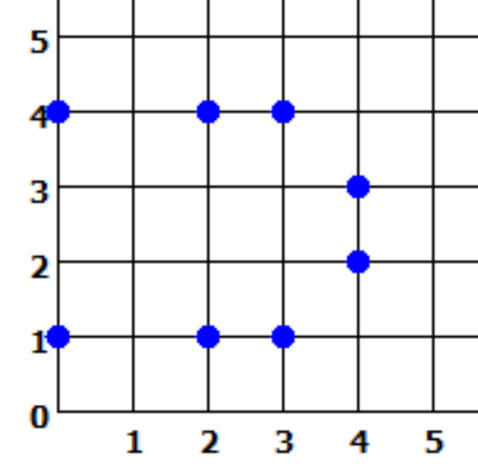
\includegraphics[width=.7\linewidth]{figures/3.png}
        \caption{$E:y^2=x^3+x+1$ over $\F_5$}
        \label{figure-vis1}
        \end{subfigure}%
        \begin{subfigure}{.5\textwidth}
        \centering
        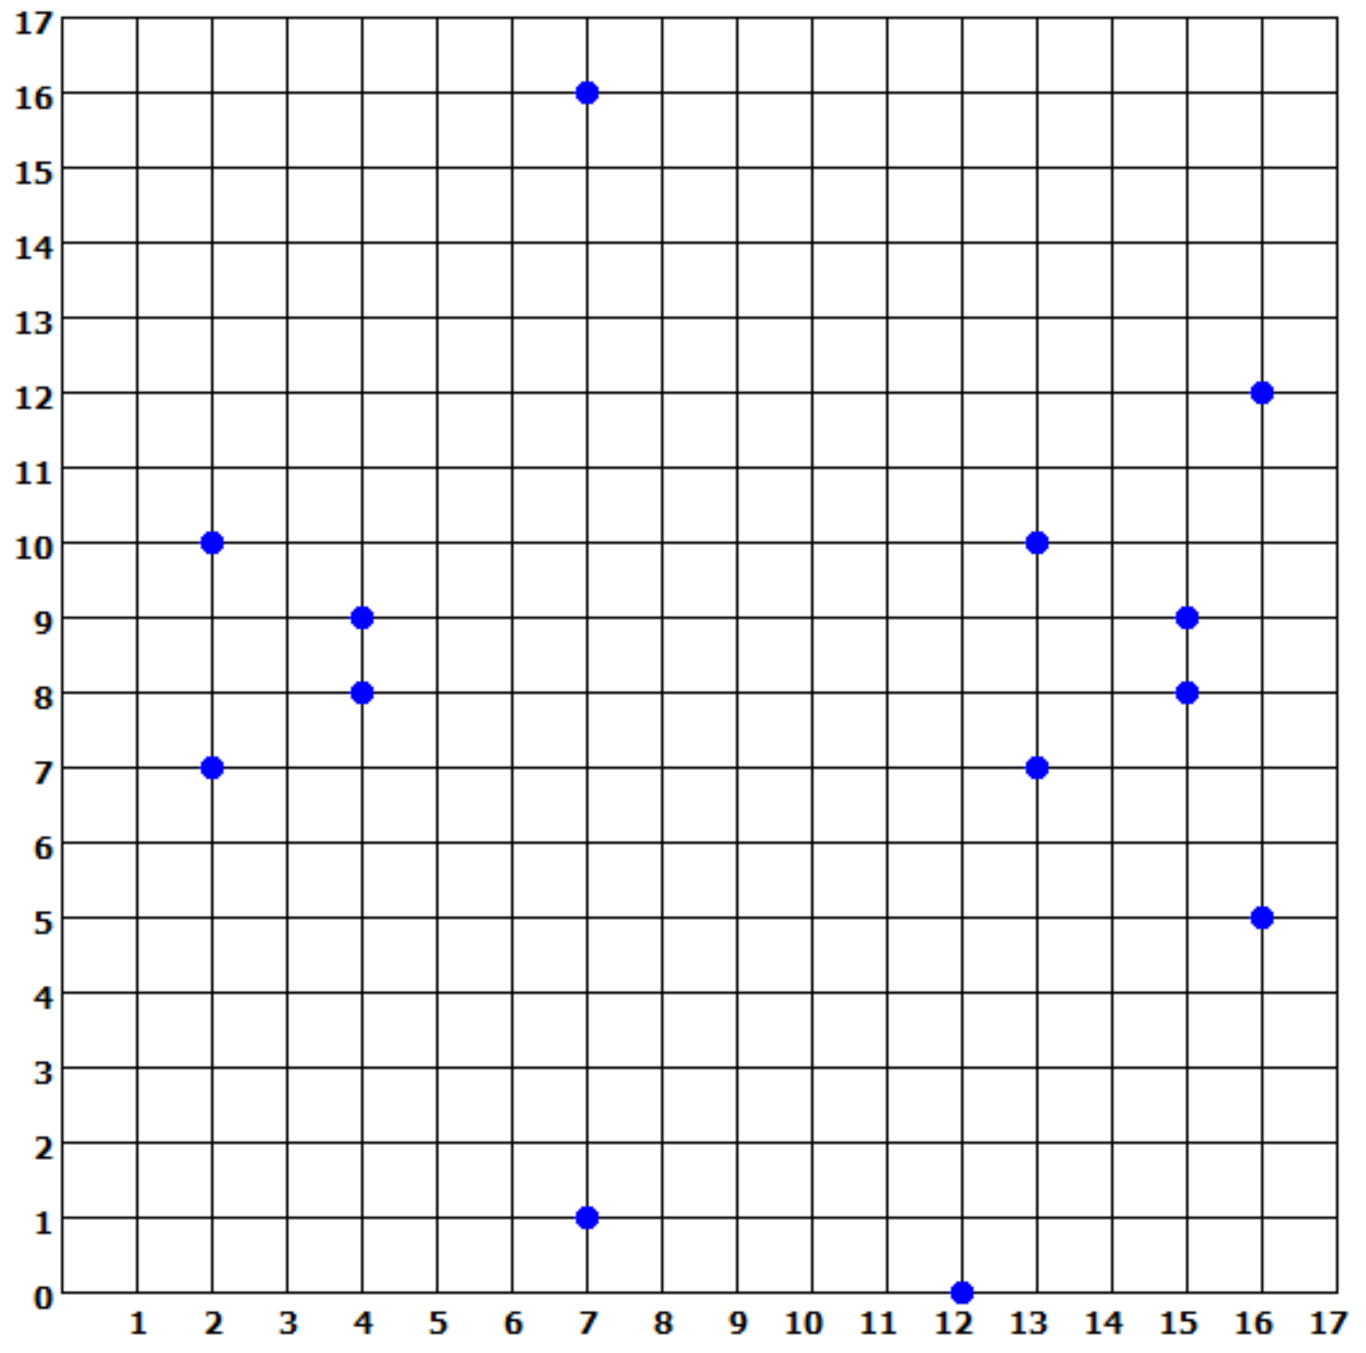
\includegraphics[width=.7\linewidth]{figures/4.png}
        
        \caption{$E:y^2=x^3+5x-3$ over $\F_{17}$}
        \label{figure-vis2}
        \end{subfigure}
    \end{figure}
    
    Since there are only $q^2$ different points in the space $\F_q^2$, so it is clear that the group $E(\F_q)$ is finite and thus finitely generated. But we are still not sure about the size of the set of $E(\F_q).$ In other words, is there an exact formula, or at least an estimate of points in $E(\F_q)$?
    \begin{remark}
        A trivial bound for $\#E(\F_q)$ is $2q+1$ since each $x$ in the Weierstrass equation produces at most two $y$'s plus the additional point at infinity of the curve.
    \end{remark}
   
    To guess the size of $E(\F_q)$, we first consider some simple cases, namely some curves of low degree. First, we consider the curve of degree 1, which is a line $y=ax+b$. In the Affine plane, we can take any values for $x$ in $\F_q$ and then the value of $y$ is completely determined. And, as for a line, there is always a point at infinity, namely the point $[1,a,0].$ Thus, there is p+1 points on the line in total. Then, we consider the curve of degree 2, the conic $$C: ax^2+bxy+cy^2+dx+ey+f=0.$$ It turns out that the set of rational points on the conics whose equations' coefficients are in $\F_q$, $C(\F_q)$, are never empty. So, we can pick a rational point on the conics C as the projective point and then project each point on the conics to a line not passing the projective point by drawing the line passing through the projective point and the point and getting the intersection point of two lines. (we also project the projective point to the line by drawing the tangent line of the conics at the projective point and getting the intersection point of two lines) Thus, we set up a one-to-one correspondence between points on the conics and points on the line. Also, the rational point on the conics are also on-to-one correspondent to the rational points on the lines. So, the number of rational points on a conics is the same as those on a line, which is $(p+1).$
    Now, before returning to our discussion of the curve $$C:y^2=f(x),$$ where $f(x)$ is a polynomial with coefficients in $\F(p)$. We substitute different values $x=0,1,...,p-1$ into $f(x)$, if $f(x)=0$, then $y$ can only be 0. If $f(x)\neq0$, then there are two possible $y$ values if $f(x)$ is a square element, and there are no $y$, if $f(x)$ is a non-square element.That is to say, if $f(x)$ is randomly distributed among the subfield $F_q$, intuitively speaking, we would expect $q+1$ points, since each value of $x$ yields either one $y$, or it has 50\% chance of yielding two $y$'s and 50\% chance of yielding no $y$. 
    In fact, Hasse and Weil confirmed this intuitive analysis. 
    \begin{theorem}\label{theorem-hasse-weil}
        If $C$ is a smooth irreducible curve of genus $g$ defined over a finite field $\F_p$, then the number of $\F_{q}$-rational points on $C$ is equal to $q+1-\epsilon$, where the error term $\epsilon$is not larger than $2g\sqrt{q}$ and $q=p^r$ for some $r$.
    \end{theorem}
    \begin{corollary}\label{Hasse-Weil}
        For all elliptic curves $E/\F_q$,
        \[|\#E(\F_p)-p-1| \leqslant 2 \sqrt{q}\]
    \end{corollary}
    \begin{proof}
        See \autoref{ssec-hasse-bound}.
    \end{proof}
    
    
    
    %%%%%%%%%%%%%%%% subsection %%%%%%%%%%%%%%%%%%%%
    \subsection{Factorization algorithm}
    
    The famous cryptosystem RSA involves the problem in number theory called prime factorisation. In this section, the traditional method and the elliptic curve version of prime factorisation algorithms are introduced. 
    
    \subsubsection{Prime or composite}
        Fermat's little theorem: if $n$ is prime, then $2^{n-1} \equiv 1$ (mod $n$). In fact, this works for any integer $a$ not divisible by $p$. So $a^{n-1} \equiv 1$ (mod $n$). It is easier to prove Fermat's little theorem using the group $\Z/n\Z$ as one gets the identity raising any element to the $(n-1)$th power. If $2^{n-1}\text{ mod }n\neq 1$, $n$ is composite. Unfortunately, the converse of Fermat's little theorem is not true, so one cannot prove that $n$ is prime in this way.
    
        To determine $a^k$ (mod $n$) where $a, k, n$ are positive integers, write $k$ as a binary number, that is 
        $$k = \sum^{r}_{i=1} c_i 2^i \quad \text{ where } c_i \in \{0, 1\}$$
        where $r \leq \log_2{k}$. Then $a^k = \prod_{i \text{ s.t. } c_i \neq 0} a^{2^i}$. Define the iterative process 
        $$A_0 = a, \quad A_{n+1} = A_n^2 \text{ (mod } n\text{)}$$
        We have $a^k \equiv \prod_{i \text{ s.t. } c_i \neq 0} A_i \text{ (mod } n\text{)}$, so it takes at most $2r \leq 2\log_2{k}$ operations ($r$ operations for finding $A_i$ and at most $r$ operations for multiplying all necessary $A_i$). This is called the fast powering algorithm, with a logarithmic complexity. 

    \subsubsection{Greatest common divisors}
        The Euclidean algorithm is a quick way to determine $\text{gcd}(a, b)$, letting $a = r_0, b = r_1$, we can apply Euclidean division repeatedly: 
        $$r_{i-1} = r_i q_i + r_{i+1} \quad \text{where } 0 \leq r_{i+1} < r_i$$
        $b = r_1 > r_2 > r_3 > \cdots$ so this process terminates when $r_{n+2} = 0$ and the final equation is $r_n = r_{n+1} q_{n+1}$. It can be proved that $r_{n+1} = \gcd(a, b)$. 
        \begin{theorem}
            The Euclidean algorithm $O(\log n)$. The number of steps required for computing $\gcd(a, b)$ with Euclidean algorithm is $\log_2(\max\{2a, 2b\})$.
        \end{theorem}
        \begin{proof}
            First note that for all $i$, $r_{i+1} \leq \frac{1}{2} r_{i-1}$ ($*$). From the relation $r_{i-1} = r_i q_i + r_{i+1}$ we have 
            $$r_{i+1} = r_{i-1} - r_i q_i$$
            By the decreasing nature of the sequence $r_i$ ($b = r_1 > r_2 > r_3 > \cdots$), there is nothing to prove if $r_i \leq \frac{1}{2} r_{i-1}$. So assume $r_i > \frac{1}{2} r_{i-1}$, 
            $$r_{i+1} = r_{i-1} - r_i q_i < r_{i-1} - \frac{1}{2} r_{i-1} q_i = r_{i-1} \left(1-\frac{1}{2} q_i\right)$$
            If $q_i = 0$, $r_{i-1} = r_{i+1}$, we get a contradiction. So $q_i \geq 1$ and $r_{i+1} \leq \frac{1}{2}r_{i-1}$.  Using ($*$) one obtains
            $$r_{2i} < \frac{1}{2} r_{2(i-1)} < \cdots < \frac{1}{2^{i-1}}r_1 = \frac{1}{2^{i-1}} b$$
            If $2^{i-1} \geq b$ ($**$), then $r_{2i} < 1$, the only such nonnegative integer is $0$. ($**$) happens when $i \geq 1+\log_2{b} = \log_2(2b)$. So the Euclidean algorithm terminates after $2\log_2(2b)$ steps. But one may begin with $b=r_0, a=r_1$ instead, so we take the maximum of $2a, 2b$. 
        \end{proof}
        The prime factorization of small $a,b $ is a feasible plan, but may not be efficient for larger numbers. 
        
    \subsubsection{Pollard's $p-1$ algorithm}
        For small number $n$, one can find its prime factorization by listing all primes smaller than $\sqrt{n}$ and pull out factors by brute-force. The time complexity grows exponentially with $n$ so this is not a wise algorithm for larger numbers.
        
        Suppose $n = pq$ where $p$ is prime, by Fermat's little theorem, $a^{p-1} \equiv 1$ (mod $p$) if $a$ is coprime to $p$. So $a^{m(p-1)} \equiv 1$ (mod $p$) for any positive integer $m$. Namely, given $k = m(p-1)$, $a^{k} - 1 = pr$ for some integer $r$. Clearly $p | \text{gcd}(pr, pq) = \text{gcd}(a^{m(p-1)} - 1, n)$. But without knowing any factor in the beginning, we can only take a try when $k$ is a product of small primes. Usually $a$ is chosen to be $2$, but choosing any small prime that does not divide $n$ suffices.
        
        Then using the fast powering algorithm and the Euclid algorithm, one can compute $a^k - 1 $ (mod $n$) and $e= \text{gcd}(a^k - 1, n)$ within $2 \log_2(2kn)$ operations ($2 \log_2(k)$ for fast powering and $2 \log_2(2n)$ for Euclidean algorithm). If $n$ do have a prime factor $p$ with $p-1 | k$, then $p | a^k - 1$, and $e \geq p > 1$. So the following outcomes require a different approach: 
        \begin{itemize}
            \item $e = 1$ : this $k$ fails (no prime factor $p$ s.t. $p-1|k$) and we need to increase $k$
            \item $e = n$ : this is a trivial factor and we have to change choice of $a$
            \item $1 < e < n$, we have a factor of $n$, and we can write $n$ as a product of two smaller numbers. Although $e$ may not be prime, we can repeat the process on $e, n/e$ and even further until we get prime factors. 
        \end{itemize}
        The number $k$ can be chosen to be $d!$ ($d = 2, 3, \cdots$). As $d$ increases, we must eventually meet a prime factor $p$ of $n$ s.t. $p | d!$, so $\text{gcd}(a^k - 1, n) > 1$ and process terminates (unless $\text{gcd}(a^k - 1, n) = n$, but this has an extremely low probability for large $n$). So the algorithm is only efficient if there is a prime factor s.t. $p-1$ is product of small primes to small powers.

        \begin{definition}[$B$-power smooth]
            A number is called $B$-power smooth if and only if given its prime factorization $\prod^r_{i=1} p_i^{e_i}$, for each $i$, $p_i^{e_i} \leq B$.
        \end{definition}

        So Pollard's $p-1$ algorithm works well with $B$-power smooth numbers when $B$ is a relatively small number. This yields another way to pick $k$: 
        $$k = \prod_{\substack{p\text{ prime}\\ 1 \leq p \leq B}} p^{\left\lfloor \frac{\log{B}}{\log{p}} \right\rfloor}$$
        where $B$ is chosen around $10^5$ to $10^6$, and it is increased when $e=1$.
        
        If all $(\Z/p\Z)^\times$ ($p$ is prime factor of $n$) have orders divisible by a large prime $p_l$, for most choices of $a$, $e = 1$ for $k$ until $k$ increases to a value such that $p_l | k$.
        \begin{example}
            Let $n = 1329 = 347 \times 383$. $347 - 1 = 2 \times 173, \; 383 - 1 = 2 \times 191$ ($173, 191$ are all primes). Let $p_1 = 347, p_2 = 383$. So as element of $(\Z/p_i\Z, +)$, except $a \equiv 0, \pm 1 \mod p_i$, any other $a$ has order $p_i/2$ or $p_i$. That means unless it happens that $(p_1/2) | k$ or $(p_2/2) | k$, otherwise, for most $a$, $\gcd(a^k-1, n) = 1$. $p-1$ being divisible by large prime is not rare, out of $16$ primes between $300$ and $400$, there are $3$ primes $p$ ($347, 359, 383$) s.t. $p-1$ has a prime factor larger than $100$. 
        \end{example}
        This makes Pollard's algorithm on $(\Z/p\Z)^\times$ very risky. Lenstra suggested to use the group $E(\F_p)$ instead. Then not only we can choose $k$, but also the curve $E$. By \autoref{theorem-hasse}, 
        $$|E(\F_p)| = p+1 - \epsilon_p \quad \text{ where }|\epsilon_p| \leq 2 \sqrt{p}$$
        and Birch \cite{birch} showed that among the finite choices of curve $E$ over finite field, $\epsilon_p$ is spread out between $\pm 2 \sqrt{p}$. So the problem of large prime dividing some $p-1$ ($p | n$) can be solved by trying many curves $E$.
        
        The process itself is almost a copy of Pollard $p-1$ algorithm on $\Z/p\Z$, if $\left.|E(\F_p)| \right| k$, then $[k]P = \mathcal{O}$ in $E(\F_p)$. While calculating $[k]P$, we have a chance of getting a factor of $n$. But there are some technical details:
        \begin{itemize}
            \item \textbf{Requirements on $n$} We need $\gcd(n, 6) = 1$ so that $E(\F_3), E(\F_2)$ will not be involved. Because transformation into Weierstrass normal form requires $\text{char}(F_p) = p \neq 3$ and removing quadratic term for cubic of $x$ in the form requires $p \neq 2$. Also we require $n$ not to be a perfect power (checked by finding $n^{\frac{1}{m}}$ for $m \in \N$ until getting an integer or $n^{\frac{1}{m}} < 2$. In the latter case, $n$ is not a perfect power). The third requirement is that $n$ should be odd; otherwise, keep taking out factor $2$ until it becomes odd. 
            \item \textbf{Choice of elliptic curve} The Weierstrass normal form without the quadratic term in $x$ is
            $$y^2 \equiv x^3 + bx + c \pmod{n}$$ 
            One can choose the curve (i.e. choose $b, c$ randomly) first and suffer to find solution $x, y$ to this modulus equation, or one can save time by randomly choosing $b, x_1, y_1$ and let $c \equiv y_1^2 - x_1^3 - b x_1 \pmod{n}$. We define the point $P = (x_1, y_1)$ and it is on the curve. 
            \item \textbf{Computation of $[k]P$} Just like fast powering algorithm, calculating $[k]P$ by first finding $P_r = [2^r]P$ with iterations is faster. Thus we add all the $P_i$ required to get $[k]P$. But we should work on mod $n$ not on $\Q$ as the coordinates may blow up. So the duplication formulas may fail: the tangent at $Q = (x, y)$
            $$\lambda = \frac{f'(x)}{2y} \equiv \frac{2x^2 + 2ax + b}{2y} \pmod{n}$$
            either $\gcd(2y, n) = 1$ (i.e. $\gcd(y, n) = 1$ as $n$ is odd) or $\gcd(2y, n) > 1$. In the first case, $2y$ has an inverse so we are able to double $Q$. In the second case, if $\gcd(y, n) < n$, we have a nontrivial factor of $n$. But if $\gcd(y, n) = n$, we have to change $k$ or the curve $E$. Similarly when adding two points $A, B$, $\frac{y_B - y_A}{x_B - x_A}$ may not always be defined and when $1 < \gcd(x_B - x_A, n) < n$, we get a nontrivial factor of $n$.
        \end{itemize}

        \newpage
        A figure of full steps of Lenstra's algorithm is given below 
        \begin{figure}[h!]
            \centering
            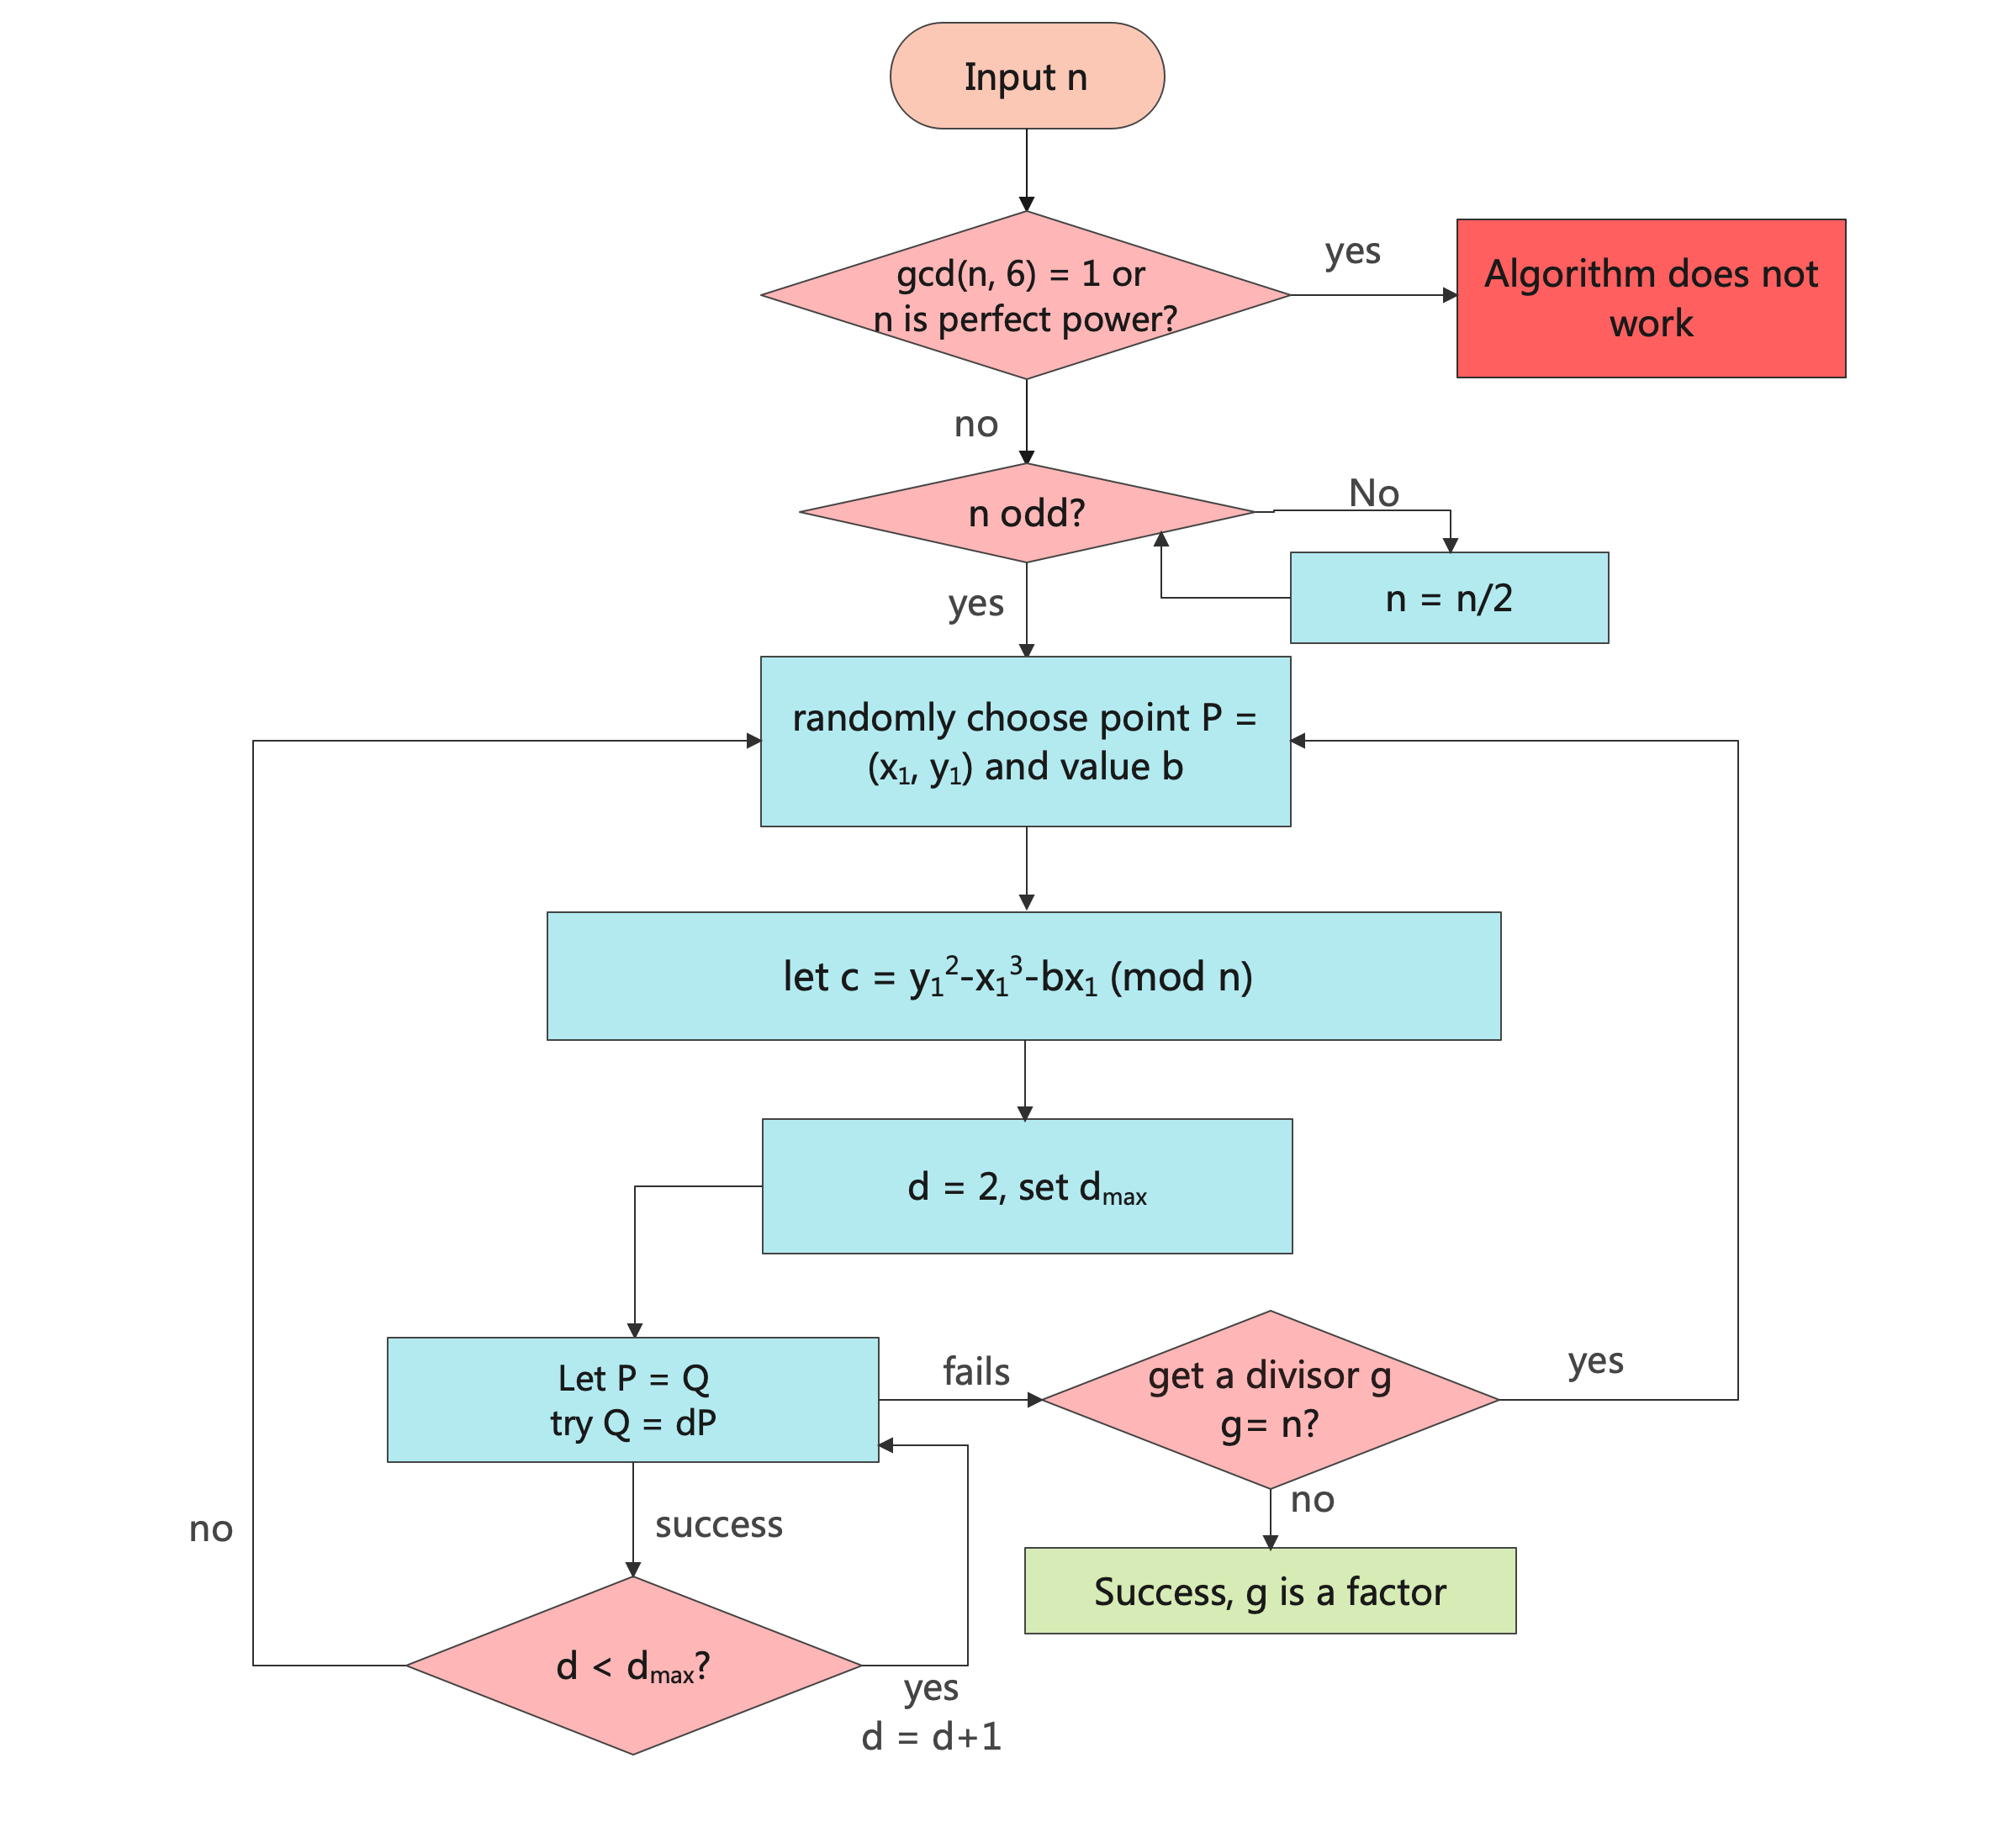
\includegraphics[scale=0.2]{figures/flow chart.png}
            \caption{Flow chart of Lenstra's idea}
            \label{fig:lenstra}
        \end{figure}
        Note in this algorithm, the value of $[k]P$ does not really matter, the factor is obtained when calculation of $[k]P$ fails. This is the funny part, you can only succeed (get a factor of $n$) if you fail.

        \textbf{Efficiency:} Just like Pollard's $p-1$ algorithm, the algorithm works well if $|E(\F_p)|$ is $B$-smooth. If $E$ is randomly chosen, this has probability $u^{-u}$ where $u = \frac{\ln{p}}{\ln{B}}$. And using this probability, estimate the complexity of Lenstra's algorithm is $O(e^{E\sqrt{r \log{r}}})$ where $r$ is the number of bits in $n$ and $E$ is the smallest number s.t. $(d_{\max})!$ is $E$-smooth.
    
    
    %%%%%%%%%%%%%%%% subsection %%%%%%%%%%%%%%%%%%%%
    \subsection{Cryptography}
    
    A cryptosystem consists of a function $f$ that can encipher (or encrypt), a message $m$, and $e = f(m)$ is sent to the receiver. In \textit{classical cryptosystem} (or private key cryptosystem), $f$ is kept secret (more precisely, the parameters of $f$, also called \textit{encipher key}, are kept secret). With the encipher key, one can easily find a \textit{decipher key} to decipher the message by applying $f^{-1}$ to $e$. For example, if $f(m) = m + 2 \mod n$, then encipher key is $2$ and decipher key is $-2$, then $f^{-1}(e) = e-2 \mod n$. But without the key, it should be difficult to find $f^{-1}$. So two parties must meet once to exchange the keys before communicating online safely. 

    However, for security concerns, two parties using a classical cryptosystem usually update the keys frequently to avoid being cracked. But frequent exchanges of keys (in person, or via a trusted third party) is very inconvenient. So \textit{public key cryptosystems} are created, which can potentially solve this. Encipher keys are no longer kept private, but $f$ is changed to a \textit{trapdoor} function (such function is difficult to invert. Ideally, the decryption complexity without a decryption key should be polynomial-time, and the complexity with the key should be logarithmic). Only with the help of a specific decipher key, one can invert the function and decode the encrypted message. Key steps
    \begin{enumerate}
        \setlength\itemsep{0.2em}
        \item Find some decipher key, for example, some large numbers. Use them to construct a trapdoor function $f$. 
        \item Publish $f$ (or the encipher keys) so that everyone who wants to send message to you can encrypt the message
        \item After receiving the message, use decipher key to decode. 
    \end{enumerate}
    There is no need for two parties to meet in person. The disadvantage if public-key cryptosystem is that decrypting or encrypting takes longer and the capacity of the message is small. So a public key cryptosystem is always used to exchange keys for the private key cryptosystem, and the latter is used for main communications. 
    \subsubsection{RSA} 
    The RSA is a public-key cryptosystem, we will skip the process of encoding a string message like ``elliptic" to a number. Assume the information being exchanged is just a number $P$, here are the steps for constructing the RSA
    \begin{itemize}
        \item Choose two large primes randomly $p, q$ (not too close) and let $N = pq$. 
        \item Choose a random integer $e$ s.t. $\gcd(e, \phi(N)) = 1$ where $\phi(N)$ is the number of integers between $1, N$ that is coprime to $N$ and for $N = pq$, $\phi(N) = (p-1)(q-1)$. 
        \item With $p, q$, it is easy to find $d = e^{-1}\pmod{\phi(N)}$. The number $d$ is the decipher key for our algorithm
        \item Publish $N, e$ (encipher keys) but conceal $d, p, q$.
        \item Encryption: $f(P) = P^e \; (\text{mod } N)$, decryption: $f^{-1}(C) = C^d \; (\text{mod } N)$
    \end{itemize}
    Two functions in the last step are indeed the inverse of each other 
    $$f^{-1} (f(P)) = P^{de} \; (\text{mod } N) = P \; (\text{mod } N)$$
    as $d, e$ are the inverse of each other in $\Z/N\Z$. It is believed that without $p, q$, one cannot find $d$ easily. And two powerful methods for factorization (in order to compute $p, q$) are the elliptic curve factorization (described in the previous section) and the number field sieve: 
    \begin{itemize}
        \item Number field sieve takes approximately $e^{c \sqrt[3]{\log{N}}}$ of time where $c$ is some small constant. And numbers considered impossible to be factored are $N \geq 2^{2048} \approx 10^{617}$. It works faster than the elliptic curve factorization if $p \approx q$. 
        \item If $p \ll q$, the elliptic curve method takes about $e^{c\sqrt{\log{p}}}$, and it is faster than the number field sieve. Yet, the number of bits required for $N$ to be infeasible to decompose is huge. 
    \end{itemize}
    
    While the difficulty of factorizing large primes is the foundation of RSA, the difficulty for finding $m$ s.t. $a^m \equiv b (\text{mod } p)$ allows us to build a trapdoor function for \textit{discrete logarithm problem}(DLP).
    
    When studying prime factorization, we changed the scope from the group $(\Z/p\Z)^\times$ to $C(\F_p)$ which improved efficiency. Similarly, DLP can be used on any group. With group $G = C(\F_p)$, we get \textit{elliptic curve discrete logarithm problem} (ECDLP) where given $P, Q \in C(\F_p)$, it is believed that finding $m$ s.t. $[m]P = Q$ is difficult (the idea of introducing elliptic curves to DLP is provided by Neal Koblitz and Victor Miller in mid-1980s). 
    
    The ECDLP may be harder to crack compared to DLP because the powerful tool to solve DLP, index calculus, relies on the fact that $\Q^\times_\{(p)\} := \{a/b \in \Q \, : \, p \nmid b\}^\times$ is infinitely generated by "small" generators. But by Mordell's theorem, $C(\Q)$ is finitely generated, so the index calculus fails. For ECDLP,  any $p > 2^{200}$ is considered secure instead of requiring $p > 2^{2048}$.
    
    Cryptography is a field that still lacks theoretical support, for example, it is hard to prove if a trapdoor function is really difficult to invert, or maybe such an inversion algorithm is not yet invented. The complexity of an algorithm also requires rigorous proof. And there are various schemes of cryptosystems, each with its own strength (more efficient than others in some cases).
    
    
    %%%%%%%%%%%%%%%%%%%%%%%%%%%%%%%%%%%%%%%%%%%%%
    %%%%%%%%%%%%%%%% Section %%%%%%%%%%%%%%%%%%%%
    %%%%%%%%%%%%%%%%%%%%%%%%%%%%%%%%%%%%%%%%%%%%%
    \section{The $p$-Riemann Hypothesis}
        The prominent and difficult Riemann Hypothesis was first presented by Riemann himself in 1859 \cite{riemann_1859_ueber}, concerning the real part of the nontrivial zeros of the analytic continuation of the zeta function
        \[\zeta(s)=\sum_{n\geqslant 1}\frac{1}{n^s}\]
        The mathematical genius Euler proved that
        \[\zeta(s)=\prod_{p\text{ prime}}\frac{1}{1-p^{-s}}\]
        in 1740. 
        
        While people had no idea about how one might prove or disprove the Riemann Hypothesis, Emil Artin studied a generalized version of this zeta function. Let $R$ be an algebra of finite type over $\Z$ (we don't care what this means). Then for any maximal ideal ideal $\mathfrak m\lhd R$, the residue field $R/\mathfrak m$ is finite. Artin then defined a generalized zeta function by
        \[\zeta_R(s)=\prod_{\mathfrak m\text{ maximal}}\frac{1}{1-\#(R/\mathfrak m)^{-s}}\]
        Note that if $R=\Z$ then the maximal ideals are of the form $p\Z$ and then $\zeta_\Z(s)$ is just the regular Riemann zeta function. Unfortunately this definition did not provide the mathematicians with anything special or useful for Riemann Hypothesis \cite{oort_2014_wei}. In his Ph.D. thesis, Emil Artin presented an analogous definition of the zeta function $Z(V;T)$ on algebraic curves $V$ over finite fields \cite{Artin1924}. This zeta function is also called the Hasse–Weil zeta function. This new zeta function then proved to be fruitful, and led to some fruitful developments in geometry and number theory.
        
        With this new zeta function on algebraic curves over a finite field $\F_q$ of characteristic $p>0$, German mathematicians were able to produce a similar version of Riemann Hypothesis, called the \textit{$p$-Riemann Hypothesis}, on the properties of $Z(V;T)$. The zeta function $Z(V;T)$ is essentially a generating function of the sizes of the sets $V(\F_{q^n})$ representing the $\F_{q^n}$-rational points in $V$. 
        
    %%%%%%%%%%%%%%%% subsection %%%%%%%%%%%%%%%%%%%%
    \subsection{The Hasse bound}\label{ssec-hasse-bound}
        Suppose $E/\F_q$ is an elliptic curve and $q$ is a power of some prime $p$. As mentioned in \autoref{ssec-bound-easy}, one might be interested in bounding the number of $\F_q$-rational points in $E$. \autoref{Hasse-Weil} was conjectured by Artin in his Ph.D. thesis, and proven by Hasse latter in 1930s.
        \begin{theorem}[Hasse bound]\label{theorem-hasse}
            Let $E/\F_q$. Then
            \[|\# E(\F_q)-q-1|\leqslant 2\sqrt{q}\]
        \end{theorem}
        \begin{proof}
            Let $\varphi_q:E\to E$ be the $q$th Frobenius map. Since the Galois group $\Gal(\overline{\F_q}/\F_q)$ is topologically generated by the Frobenius endomorphism $F:x\mapsto x^q$ (that the cyclic group $\langle F\rangle$ is dense in $\Gal(\overline{\F_q}/\F_q)$ with respect to its Krull topology).; equivalently, the restriction of every $\s\in\Gal(\overline{\F_q}/\F_q)$ to $\F_{q^n}$ is a power of $F$. Thus,
            \[P\in E(\F_q)=E^{\Gal(\overline{\F_q}/\F_q)}\text{ if and only if }\varphi_q(P)=\varphi\]
            which means $E(\F_q)=\ker(1-\varphi_q)$. By \autoref{theorem-frob-sep} and \autoref{theorem-size-ker-iso}, $\# E(\F_q)=\deg(1-\varphi_q)$. Since $\deg [1]=1^2=1$ and $\deg \varphi_q=q$, by \autoref{corollary-deg-pos-quadratic} and \autoref{lemma-cauchy-schwartz},
            \[|\# E(\F_q)-q-1|=|\deg(1-\varphi_q)-\deg[1]-\deg\varphi_q|\leqslant 2\sqrt{\deg[1]\cdot\deg\varphi_q}=2\sqrt{q}\]
            which completes the proof.
        \end{proof}
        \begin{example}
            Let $f(x)=ax^3+bx^2+cx+d$ be a cubic with distinct roots in $\F_q[x]$. Let $\chi:\F_q^\times\to\{\pm 1\}$ be the character which determines if an element is a square in $\F_q$. One immediately sees that the number of solutions to $E:y^2=f(x)$ is (with the point at infinity)
            \[\# E(\F_q)=1+\sum_{x\in \F_q}\left[1+\chi\left(f(x)\right)\right]=1+q+\sum_{x\in\F_q}\chi\left(f(x)\right)\]
            which suggests
            \[\left|\sum_{x\in\F_q}\chi\left(f(x)\right)\right|\leqslant 2\sqrt{q}\]
            by \autoref{theorem-hasse}.
        \end{example}
    %%%%%%%%%%%%%%%% subsection %%%%%%%%%%%%%%%%%%%%
    \subsection{Weil conjectures}
        The Weil conjectures consist of several conjectures concerning the properties of the zeta function defined on algebraic varieties (which was primarily defined by Emil Artin in his Ph.D. thesis, mentioned in \autoref{sec-intro}). Given a smooth projective variety $V/\F_q$, we define similarly the set of $\F_{q^r}$-rational points on $V$, denoted by $N_r=\# V(\F_{q^r})$.
        \begin{definition}
            The \textit{zeta function of $V/\F_q$} is the power series
            \[Z(V/\F_q;T)=\exp\left(\sum_{r=1}^\infty \frac{N_r}{r}T^r\right)\]
            where the exponential of a power series with no constant term is defined by
            \[\exp(F(T))=\sum_{k=0}^\infty \frac{F(T)^k}{k!}\]
        \end{definition}
        \begin{remark}
            If we know the zeta function, we could recover each $N_r$ from it:
            \[N_r=\frac{1}{(r-1)!}\left.\frac{d^r}{dT^r}\log Z(V/\F_q;T)\right|_{T=0}\]
        \end{remark}
        \begin{example}
            Let's try an easy example. Consider the projective space $V=\Pc^n$. Then the number of points in $V(\F_{q^r})$ is simply $N_r=\frac{q^{r(n+1)-1}}{q^r-1}=\sum_{i=0}^nq^{ir}$ (discard the zero tuple and dividing out the equivalence classes). Thus, we have
            \[\log Z(V/\F_q;T)=\sum_{r=1}^\infty \sum_{i=0}^n\frac{(q^iT)^r}{n}=\sum_{i=0}^n-\log(1-q^iT)\]
            where the second equality holds by exchanging the summation. Thus,
            \[Z(V/\F_q;T)=\frac{1}{(1-T)\cdots (1-q^nT)}\]
        \end{example}
        \begin{remark}
            What is the set $E(\F_{q^n})$ essentially? Similar to what was argued in \autoref{theorem-hasse}, $E(\F_{q^n})$ is the set of fixed points of the $n$th iterate of the $q$th power Frobenius map $\varphi_{q}$. Therefore, we have $\# E(\F_{q^n})=\ker(1-\varphi_q^n)$, which opens a path way to proving a particular case of the Weil conjectures Hasse used in 1936 \cite{Hasse1936}.
        \end{remark}
        The history of the Weil conjectures is also quite interesting. Hasse solved the $p$-Riemann Hypothesis for curves of genus one, i.e., elliptic curves, and proved \autoref{theorem-hasse}. Weil was aware of this result, and announced an outline of the proof for curves of genus $g$ (\autoref{theorem-hasse-weil}) in 1940, when he was a prisoner ``in a French military prison for failing to report for duty" \cite{baez_2019_the}! In 1941 Weil published a proof of \autoref{theorem-hasse-weil}. Weil then studied equations of the form
        \[a_0x_0^{m_0}+\cdots+a_rx_r^{m_r}=b\]
        over some finite fields, and when $b=0$, Weil found that
        \[\sum_{n=1}^\infty N_nT^{n-1}=\frac{d}{dT}\log\left(\frac{1}{(1-T)\cdots (1-q^rT)}\right)+(-1)^r\frac{d}{dT}\log P(T)\]
        for some polynomial $P$ \cite{milne_2016_the}. Weil then wrote, in \cite{weil_1949_numbers}, that his observation of the homogeneous equations over finite fields might lead to some ``conjectural statements", which are rephrased and restate below. These famous statements are the so-called ``Weil conjectures". A brief remark on the name of the last statement is in \autoref{remark-p-rh}.
        \begin{theorem}[Weil conjectures]
            Let $V/\F_q$ be a smooth projective variety of dimension $N$. Then
            \begin{enumerate}[\normalfont(i)]
                \item Rationality: $Z(V/\F_q;T)\in\mathbb Q(T)$.
                \item Functional equation: there is an integer $\ve$ --- the Euler characteristic of $V$ --- such that $Z(V/\F_q;1/q^NT)=\pm q^{N\ve/2}T^{\ve}Z(V/\F_q;T)$.
                \item $p$-Riemann Hypothesis:
                \[Z(V/\F_q;T)=\frac{P_1(T)P_3(T)\cdots P_{2N-1}(T)}{P_0(T)P_2(T)\cdots P_{2N}(T)}\]
                where $P_i\in\Z[T]$, $P_0(T)=1-T$ and $P_{2N}=1-q^NT$. Furthermore, each $P_i$ factors over $\C$ with roots $\alpha_{ij}$ satisfying $|\alpha_{ij}|=q^{1/2}$ for all $i, j$. The degree of $P_i$, $b_i$, is the $i$th \textup{Betti number of $V$}. 
            \end{enumerate}
        \end{theorem}
        As noted before, a baby version of these ``conjectures" was proved by Hasse in 1930s. In 1950s, Weil proved these statements for abelian varieties --- varieties with an abelian structures but, unlike elliptic curves, are of arbitrary genus and dimension. Grothendieck proved the first two statements for general projective varieties using his theory of étale cohomology, but was unable to prove the $p$-Riemann Hypothesis. In 1973, Deligne presented his first proof of Weil conjectures \cite{deligne1}; in 1980, Deligne presented another proof \cite{deligne2}. Deligne's proof was described by Gowers as a ``surprise" from Weil's belief of the need of ``standard conjectures". Deligne took a ``different route", in spite of using Grothendieck's cohomology theory \cite{gowers_2013}.
    %%%%%%%%%%%%%%%% subsection %%%%%%%%%%%%%%%%%%%%
    \subsection{Hasse's proof for elliptic curves}
        Due to the extreme difficulty of the Weil conjectures for general varieties and the level of knowledge required to understand them, we only present the proof of Weil conjectures for elliptic curves --- smooth projective varieties of genus one and dimension one. This proof is due to Hasse and was done years before Weil conjectures.
        \begin{lemma}\label{lemma-the-last}
            Let $E/\F_q$ be an elliptic curve. Let $\varphi_q$ be the $q$th power Frobenius map and suppose
            \[a=q+1-\# E(\F_q)\]
            Then
            \begin{enumerate}[\normalfont(i)]
                \item Let $\alpha,\beta\in\C$ be roots of $T^2-aT+q$. Then $\beta=\bar{\alpha}$ and $|l\alpha|=|\beta|=\sqrt{q}$ and for all $n\geqslant 1$,
                \[N_n=\# E(\F_{q^n})=q^n+1-\alpha^n-\beta^n\]
                \item The characteristic polynomial of $\varphi$ is $T^2-aT+q$.
            \end{enumerate}
        \end{lemma}
        \begin{proof}
            By \autoref{theorem-frob-sep}, $1-\varphi_q$ is separable and by \autoref{theorem-size-ker-iso},
            \[\# E(\F_q)=\#\ker(1-\varphi_q)=\deg(1-\varphi_q)\]
            By \autoref{theorem-map-deg-tr}, for any prime $l\neq p$
            \[\det(\varphi_{q,l})=\deg\varphi_q=q,\quad\operatorname{tr}(\varphi_{q,l})=1+\deg\varphi_q-\deg(1-\varphi_q)=1+q-\# E(\F_q)=a\]
            Thus by the degree-trace formula, $\varphi_{p,l}$ has characteristic polynomial $\det(T-\varphi_{p,l})=T^2-aT+q$, which factors over $\C$ as $(T-\alpha)(T-\beta)$.
            
            (i) Since for all $m/n\in\mathbb Q$, if $T=m/n$ then by \autoref{theorem-map-deg-tr},
            \[\det(T-\varphi_{p,l})=\frac{\det(m-n\varphi_{p,l})}{n^2}=\frac{\deg(m-n\varphi_{p,l})}{n^2}\geqslant 0,\]
            the quadratic function is also nonnegative for all reals. Thus, the roots must be the same or they must be two complex conjugates. In either case, we have $|\alpha|=|\beta|$. But since $\alpha\beta=\det(\varphi_{p,l})=q$, we get $|\alpha|=|\beta|=\sqrt{q}$.
            
            Similarly, $E(\F_{q^n})$ is the fixed field of $\varphi_{q}^n$. Then as $\varphi_{p,l}$ is equivalent to $\operatorname{diag}(\alpha,\beta)$ or $J_2(\alpha)$, the Jordan canonical normal form of $\varphi_{p,l}^n$ is always $\operatorname{diag}(\alpha^n,\beta^n)$ or $J_2(\alpha^n)$. Thus,
            \[\# E(\F_{q^n})=\deg(1-\varphi_{q}^n)=\det(1-\varphi_{q,l}^n)=1-\alpha^n+\beta^n+q^n\]
            
            (ii) We have by Cayley–Hamilton,
            \[\deg(\varphi_q^2-a\varphi_q+q)=\det(\varphi_{q,l}^2-a\varphi_{q,l}+q)=0\]
            which by the positive definiteness of the quadratic form $\deg$, $\varphi_q^2-a\varphi_q+q$=0.
        \end{proof}
        \begin{theorem}[Weil conjectures for elliptic curves]\label{theorem-the-last}
            Let $E/\F_q$ be an elliptic curve. Then there is an $a\in\Z$ such that
            \[Z(E/\F_q;T)=\frac{1-aT+qT^2}{(1-T)(1-qT)}\]
            and (the Euler characteristic is zero; which is already known since $2-2g=0$)
            \[Z(E/\F_q;1/qT)=Z(E/\F_q;T)\]
            and finally
            \[1-aT+qT^2=(1-\alpha T)(1-\beta T),\quad|\alpha|=|\beta|=\sqrt{q}\]
        \end{theorem}
        \begin{proof}
            With all our works, the proof is surprisingly easy.
            \begin{align*}
                \log Z(E/\F_q;T)={}&\sum_{n=1}^\infty\frac{N_nT^n}{n} &\text{by definition}\\
                ={}&\sum_{n=1}^\infty\frac{(1-\alpha^n-\beta^n+q^n)T^n}{n}&\text{by \autoref{lemma-the-last}}\\
                ={}&-\log(1-T)+\log(1-\alpha T)\\
                &+\log(1-\beta T)-\log(1- qT)
            \end{align*}
            Thus,
            \[Z(E/\F_q;T)=\frac{(1-\alpha T)(1-\beta T)}{(1-T)(1-qT)}\]
            and the other results are then obvious.
        \end{proof}
        \begin{remark}\label{remark-p-rh}
            Define a function $\zeta_{E/\F_q}(s)$ on $\C$ to be
            \[\zeta_{E/\F_q}(s)=Z(E/\F_q;q^{-s})=\frac{1-aq^{-s}+q^{1-s}}{(1-q^{-s})(1-q^{1-s})}\]
            Then we have $\zeta_{E/\F_q}(s)=\zeta_{E/\F_q}(1-s)$, which is derived from the functional equation. Furthermore, $\zeta_{E/\F_q}(s)=0$ if and only if $q^{-s}=\alpha$ or $\beta$. This means $|q^{s}|=q^{\Re(s)}=\sqrt{q}$ or $\Re(s)=\frac{1}{2}$. This why the last statement is called the $p$-Riemann Hypothesis!
        \end{remark}
        \newpage
        \section{References}
        \nocite{*}
        \renewcommand{\section}[2]{\vskip 0.01em}
        \printbibliography
\end{document}